% !TeX spellcheck = sl_SI
% vim: set spell spelllang=sl:
% za preverjanje črkovanja, če se uporablja Texstudio ali vim
\documentclass[12pt,a4paper,twoside]{article}
\usepackage[utf8]{inputenc} 


% pravilno razpoznavanje unicode znakov

% NASLEDNJE UKAZE USTREZNO POPRAVI
\newcommand{\program}{Matematika} % ime studijskega programa
\newcommand{\imeavtorja}{Anja Kišek} % ime avtorja
\newcommand{\imementorja}{prof.~dr.~Sandi Klavžar} % akademski naziv in ime mentorja, uporabi poln naziv, prof.~dr.~, doc.~dr., ali izr.~prof.~dr.
\newcommand{\imesomentorja}{} % akademski naziv in ime somentorja, če ga imate
\newcommand{\naslovdela}{Karakterizacije kografov in algoritma za izračun varnostne dominacije na kografih}
\newcommand{\letnica}{2020} % letnica magistriranja
\newcommand{\opis}{Delo obravnava pregled do sedaj znanih karakterizacij kografov ter implementira dva algoritma za izračun varnostnodominantnega števila na kografih}  % Opis dela v eni povedi. Ne sme vsebovati matematičnih simbolov v $ $.
\newcommand{\kljucnebesede}{kograf\sep kodrevo\sep varnostnodominantno število\sep dominantno število\sep popoln graf\sep linearen algoritem} % ključne besede, ločene z \sep, da se PDF metapodatki prav procesirajo
\newcommand{\keywords}{cograph\sep cotree\sep security domination number\sep domination number\sep perfect graph\sep linear algorithm} % ključne besede v angleščini
\newcommand{\organization}{Univerza v Ljubljani, Fakulteta za matematiko in fiziko} % fakulteta
\newcommand{\literatura}{literatura}  % pot do datoteke z literaturo (brez .bib končnice)
\newcommand{\sep}{, }  % separator med ključnimi besedami v besedilu
% KONEC PODATKOV

\usepackage{bibentry}         % za navajanje literature v programu dela s celim imenom
\nobibliography{\literatura}
\newcommand{\plancite}[1]{\item[\cite{#1}] \bibentry{#1}} % citiranje v programu dela

\usepackage{adjustbox}
\usepackage{filecontents}  % za pisanje datoteke s PDF metapodatki
\usepackage{silence} \WarningFilter{latex}{Overwriting file}  % odstrani annoying warning o obstoju datoteke
% datoteka s PDF metapodatki, zgenerira se kot magisterij.xmpdata
\begin{filecontents*}{\jobname.xmpdata}
  \Title{\naslovdela}
  \Author{\imeavtorja}
  \Keywords{\kljucnebesede}
  \Subject{\opis}
  \Org{\organization}
\end{filecontents*}

\usepackage[a-1b]{pdfx}  % zgenerira PDF v tem PDF/A-1b formatu, kot zahteva knjižnica
\hypersetup{bookmarksopen, bookmarksdepth=3, colorlinks=true,
  linkcolor=black, anchorcolor=black, citecolor=black, filecolor=black,
  menucolor=black, runcolor=black, urlcolor=black, pdfencoding=auto,
  breaklinks=true, psdextra}

\usepackage[slovene]{babel}  % slovenščina
\usepackage[T1]{fontenc}     % naprednejše kodiranje fonta
\usepackage{amsmath,amssymb,amsfonts,amsthm} % matematični paketi
%\usepackage[dvipsnames,usenames]{color} % barve
\usepackage{graphicx}     % za slike
\usepackage{emptypage}    % prazne strani so neoštevilčene, ampak so štete
\usepackage{units}        % fizikalne enote kot \unit[12]{kg} z polovico nedeljivega presledka, glej primer v kodi
\usepackage{makeidx}      % za stvarno kazalo, lahko zakomentiraš, če ne rabiš
\makeindex                % za stvarno kazalo, lahko zakomentiraš, če ne rabiš
% oblika strani
\usepackage[
  top=3cm,
  bottom=3cm,
  inner=3.5cm,      % margini za dvostransko tiskanje
  outer=2.5cm,
  footskip=40pt     % pozicija številke strani
]{geometry}

% VEČ ZANIMIVIH PAKETOV
% \usepackage{array}      % več možnosti za tabele
% \usepackage[list=true,listformat=simple]{subcaption}  % več kot ena slika na figure, omogoči slika 1a, slika 1b
% \usepackage[all]{xy}    % diagrami
% \usepackage{doi}        % za clickable DOI entrye v bibliografiji
% \usepackage{enumerate}     % več možnosti za sezname

% Za barvanje source kode
\usepackage{minted}
\renewcommand\listingscaption{Program}

% Za pisanje psevdokode
\usepackage[noend]{algpseudocode}  % za psevdokodo
\usepackage{algorithm}
\floatname{algorithm}{Algoritem}
\renewcommand{\listalgorithmname}{Kazalo algoritmov}

% DRUGI TVOJI PAKETI:


\usepackage{enumitem}
\setlength{\overfullrule}{50pt} % označi predlogo vrstico
\pagestyle{plain}               % samo številka strani na dnu, nobene glave / noge

% ukazi za matematična okolja
\theoremstyle{definition} % tekst napisan pokončno
\newtheorem{definicija}{Definicija}[section]
\newtheorem{primer}[definicija]{Primer}
\newtheorem{opomba}[definicija]{Opomba}
\newtheorem{aksiom}{Aksiom}

\theoremstyle{plain} % tekst napisan poševno
\newtheorem{lema}[definicija]{Lema}
\newtheorem{izrek}[definicija]{Izrek}
\newtheorem{trditev}[definicija]{Trditev}
\newtheorem{posledica}[definicija]{Posledica}

\numberwithin{equation}{section}  % števec za enačbe zgleda kot (2.7) in se resetira v vsakem poglavju


 %%% TIKZ
\usepackage{tikz}
\usetikzlibrary{patterns}


% Matematični ukazi
\newcommand{\R}{\mathbb R}
\newcommand{\N}{\mathbb N}
\newcommand{\Z}{\mathbb Z}
\renewcommand{\C}{\mathbb C}
\newcommand{\Q}{\mathbb Q}

% \DeclareMathOperator{\tr}{tr}  % morda potrebuješ operator za sled ali kaj drugega?

% bold matematika znotraj \textbf{ }, tudi v naslovih, kot \omega spodaj
\makeatletter \g@addto@macro\bfseries{\boldmath} \makeatother

% Poimenuj kazalo slik kot ``Kazalo slik'' in ne ``Slike''
\addto\captionsslovene{
  \renewcommand{\listfigurename}{Kazalo slik}%
}

% če želiš, da se poglavja začnejo na lihih straneh zgoraj
% \let\oldsection\section
% \def\section{\cleardoublepage\oldsection}

%%%%%%%%%%%%%%%%%%%%%%%%%%%%%%%%%%%%%%%%%%
%%%%%%           DOCUMENT           %%%%%%
%%%%%%%%%%%%%%%%%%%%%%%%%%%%%%%%%%%%%%%%%%

\begin{document}

\pagenumbering{roman} % začnemo z rimskimi številkami
\thispagestyle{empty} % ampak na prvi strani ni številke

\noindent{\large
UNIVERZA V LJUBLJANI\\[1mm]
FAKULTETA ZA MATEMATIKO IN FIZIKO\\[5mm]
\program\ -- 2.~stopnja}
% ustrezno dopolni za IŠRM
\vfill

\begin{center}
  \large
  \imeavtorja\\[3mm]
  \Large
  \textbf{\MakeUppercase{\naslovdela}}\\[10mm]
  \large
  Magistrsko delo \\[1cm]
  Mentor: \imementorja \\[2mm] % ustrezno popravi spol
%   Somentor: \imesomentorja   % dodaj, če potrebno
\end{center}
\vfill

\noindent{\large Ljubljana, \letnica}

\cleardoublepage

%% IZJAVA O AVTORSTVU
%\pdfbookmark[1]{Izjava o avtorstvu}{izjava} % bookmark v PDF, \pdfbookmark[nivo]{text}{label}
%
%% izjava: po potrebi spremeni v žensko obliko
%\setlength\topsep{0pt}
%\setlength\parskip{0pt}
%\begin{center}
%  \textbf{Univerza v Ljubljani} \\
%  \textbf{Fakulteta za matematiko in fiziko}
%
%  \vfill
%
%  \underline{Izjava o avtorstvu, istovetnosti tiskane in elektronske verzije magistrskega dela in} \\
%  \underline{objavi osebnih podatkov študenta}
%
%  \vfill
%
%  \setlength\topsep{0pt}
%  \setlength\parskip{0pt}
%  \begin{flushleft}
%    Spodaj podpisani študent \imeavtorja{} avtor magistrskega dela (v nadaljevanju: pisnega
%    zaključnega dela študija) z naslovom:
%  \end{flushleft}
%
%  \vfill
%
%  \textbf{\naslovdela}
%
%  \vfill
%
%  IZJAVLJAM
%\end{center}
%
%\begin{enumerate}[1. ]a
%  \item \emph{Obkrožite eno od variant a) ali b)}
%  \begin{enumerate}[a)]
%    \item da sem pisno zaključno delo študija izdelal samostojno;
%    \item da je pisno zaključno delo študija rezultat lastnega dela več kandidatov in izpolnjuje
%      pogoje, ki jih Statut UL določa za skupna zaključna dela študija ter je v zahtevanem deležu
%      rezultat mojega samostojnega dela;
%  \end{enumerate}
%  pod mentorstvom IZPOLNI. % dopiši \imementorja v rodilniku
%%   \\ in somentorstvom IZPOLNI. % dopiši \imesomentorja v rodilniku
%  \item da je tiskana oblika pisnega zaključnega dela študija istovetna elektronski obliki
%    pisnega zaključnega dela študija;
%  \item da sem pridobil vsa potrebna dovoljenja za uporabo podatkov in avtorskih del v pisnem
%    zaključnem delu študija in jih v pisnem zaključnem delu študija jasno označil;
%  \item da sem pri pripravi pisnega zaključnega dela študija ravnal v skladu z etičnimi načeli in,
%    kjer je to potrebno, za raziskavo pridobil soglasje etične komisije;
%  \item da soglašam, da se elektronska oblika pisnega zaključnega dela študija uporabi za preverjanje
%    podobnosti vsebine z drugimi deli s programsko  opremo za preverjanje podobnosti
%    vsebine, ki je povezana s študijskim informacijskim sistemom fakultete;
%  \item da na UL neodplačno, neizključno, prostorsko in časovno neomejeno prenašam pravico shranitve
%    avtorskega dela v elektronski obliki, pravico reproduciranja ter pravico dajanja pisnega
%    zaključnega dela študija na voljo javnosti na svetovnem spletu preko Repozitorija UL;
%  \item da dovoljujem objavo svojih osebnih podatkov, ki so navedeni v pisnem zaključnem delu študija
%    in tej izjavi, skupaj z objavo pisnega zaključnega dela študija.
%\end{enumerate}
%
%\vfill
%
%\noindent
%Kraj:  \hfill   Podpis študenta: \phantom{prostor za podpis}
%
%\vfill
%
%\noindent
%Datum:
%
%\cleardoublepage
%% END IZJAVA O AVTORSTVU

% zahvala
\pdfbookmark[1]{Zahvala}{zahvala} %
\section*{Zahvala}
Neobvezno.
Zahvaljujem se \dots
% end zahvala -- izbriši vse med zahvala in end zahvala, če je ne rabiš

\cleardoublepage

\pdfbookmark[1]{\contentsname}{kazalo-vsebine}
\tableofcontents

% list of figures
% \cleardoublepage
% \pdfbookmark[1]{\listfigurename}{kazalo-slik}
% \listoffigures
% end list of figures

\cleardoublepage

\section*{Program dela}
\addcontentsline{toc}{section}{Program dela} % dodajmo v kazalo
Mentor naj napiše program dela skupaj z osnovno literaturo. Na literaturo se
lahko sklicuje kot...

\section*{Osnovna literatura}
Literatura mora biti tukaj posebej samostojno navedena (po pomembnosti) in ne
le citirana. V tem razdelku literature ne oštevilčimo po svoje, ampak uporabljamo
okolje itemize in ukaz plancite, saj je celotna literatura oštevilčena na koncu.
\begin{itemize}
  \plancite{lebedev2009introduction}
  \plancite{gurtin1982introduction}
  \plancite{zienkiewicz2000finite}
  \plancite{STtemplate}
\end{itemize}

\vspace{2cm}
\hspace*{\fill} Podpis mentorja: \phantom{prostor za podpis}

% \vspace{2cm}
% \hspace*{\fill} Podpis somentorja: \phantom{prostor za podpis}

\cleardoublepage
\pdfbookmark[1]{Povzetek}{Abstract}

\begin{center}
\textbf{\naslovdela} \\[3mm]
\textsc{Povzetek} \\[2mm]
\end{center}
V delu obravnavamo kografe, njihovo reprezentacijo s kodrevesi in karakterizacijo kografov. Uvrstimo jih v družino popolnih grafov in raziščemo problem barvanja kografov. Poleg algoritma za barvanje navedemo nekaj algoritmov, ki zaradi strukture kodrevesa delujejo v linearnem času, med njimi dominacijo in varnostno dominacijo. Slednjo definiramo in raziščemo njene lastnosti. Obravnavamo dva neodvisna algoritma za iskanje varnostnodominantnega števila na kografih in argumentiramo njuno linearnost.

\vfill
\begin{center}
\textbf{Characterisation of cographs and two algorithms for computation of secure domination number of a cograph} \\[3mm] % prevod slovenskega naslova dela
\textsc{Abstract}\\[2mm]
\end{center}
This work studies cographs, their representation with cotrees and different characterisations. By observing their colorings, cographs are proved to be a special case of perfect graphs. In addition, some linear algorithms are presented which exploit the structure of cotrees. Security domination of a graph is introduced and some properties, crucial for its computation are presented. Two independent algorithms for security domination number of cographs are studied and their linearity is argumented.

\vfill\noindent
\textbf{Math.~Subj.~Class.~(2010):} 05C15, 05C17 , 05C57, 05C69, 05C76, 05C85 \\[1mm]
\textbf{Ključne besede:} \kljucnebesede \\[1mm]
\textbf{Keywords:} \keywords

\cleardoublepage

\setcounter{page}{1}    % od sedaj naprej začni zopet z 1
\pagenumbering{arabic}  % in z arabskimi številkami

\section{Uvod}
Struktura kografa---v nekaterih člankih poimenovan tudi komplementno reducibilen graf---je bila študirana na več različnih področjih teorije grafov, kjer so jo študirali bodisi nalašč, bodisi so jo na novo odkrili povsem po naključju. V člankih so se kografi pojavljali pod različnimi imeni, kot so $D^*$-grafi, grafi brez $P_4$, $HD$ ali dedni Daceyevi grafi (ang.~Hereditary Dacey graphs). V začetku sedemdesetih let prejšnjega stoletja je H.~Lerchs formaliziral definicijo kografov ter v članku \cite{corneil1981complement} zaobjel nekaj do tedaj znanih karakterizacij. Področje je še vedno zelo aktivno, zadnja raziskovanja pa preučujejo lastne vrednosti kografov \cite{allem2020integral}, \cite{ghorbani2019cographs}, odstranjevanja povezav in vozlišč kografov \cite{tsur2020faster}, uporabo v biologiji \cite{geiss2020reciprocal}, \cite{hellmuth2013orthology} ter druge kombinatorične in grafovske lastnosti \cite{brevsar2015cographs}, \cite{epple2020k}.

Mnoge karakterizacije kografov so se izkazale kot učinkovite za implementacijo najrazličnejših algoritmov za probleme, ki so v splošnem zelo težki problemi (barvanje grafov, iskanje minimalne dominantne množice, iskanje Hamiltonovega cikla, iskanje maksimalnih klik in neodvisnih množic, iskanje maksimalnega prirejanja), na kografih pa so rešljivi celo v linearnem času (glej~\cite{corneil1984clustering}, \cite{corneil1984cographs}, \cite{yu1993n}). Eden od teh problemov je tudi iskanje varnostnodominantnega števila za kografe.

Problem iskanja dominantnih množic in dominantnih števil sega v sredino 20. stoletja in se skozi različne variacije problema vrti okoli osnovnega vprašanja: najmanj koliko stražarjev, ki nadzorujejo svoje ter vsa sosednja vozlišča, moramo postaviti na vozlišča grafa, da bo zastražen celoten graf? Formalno je problem, kot ga obravnavamo danes, prvi predstavil Ore leta 1962 \cite{ore1962theory}, hkrati pa se je na področju teorije grafov in računske geometrije začelo raziskovanje algoritmov za njegovo računanje. Problem dominantnega števila je v splošnem NP-poln, kar je leta 1972 dokazal Karp \cite{karp1972reducibility}, sledile pa so mnoge posplošitve ter ocene za specifične grafe.  Poleg standardnega dominantnega števila $\gamma$ (zdaj uveljavljeno oznako sta vpeljala Cockayne in Hedetniemi leta 1977 \cite{cockayne1977towards})  se je raziskovalo tudi različne izpeljanke tega števila, ki opisujejo dodatne zahteve za strategijo >>varovanja<< grafa. Leta 1999 je Stewart \cite{stewart1999defend} uvedel pojem \emph{Rimskega dominantnega števila}, ki dovoljuje različne tipe dominantnih vozlišč. Izpeljavo Rimske dominacije so leta 2005 prvi predstavili Cockayne, Grobler, Grundlingh, Munganga in Vuuren v \cite{cockayne2005protection} pod imenom \emph{varnostna dominacija}, za katero je bilo izpeljanih mnogo rezultatov in algoritmov. Izračun varnostnodominantnega števila je v splošnem NP-poln, za specifične grafe pa je NP-poln tudi za dvodelne in razcepljene grafe (obstaja particija, ki vozlišča razdeli na kliko in neodvisno množico) \cite{merouane2015secure}, zvezdasto konveksne dvodelne ter dvojne tetivne grafe \cite{wang2018complexity} in tetivne dvodelne grafe \cite{pradhan2018computing}, hkrati pa je linearen na drevesih  \cite{burger2014linear}, \cite{li2017secure}, bločnih grafih \cite{pradhan2018computing} in intervalnih grafih \cite{araki2018secure}. Problem iskanja varnostnodominantne množice je mogoče zapisati tudi kot binaren program \cite{burdett2020improved}, \cite{burger2013binary}.

V tem delu se bomo najbolj posvetili linearnima algoritmoma za iskanje varnostne dominacije na kografih, ki sta bila med seboj neodvisno izdana leta 2019, to sta članek avtorjev Pradhan, Jha in Banerjee \cite{jha2019secure} ter avtorjev Araki in Yamanaka \cite{araki2019secure}.

\medskip
V drugem poglavju bomo definirali kografe in kodrevesa, navedli omenjene karakterizacije kografov ter predstavili nekaj algoritmov, ki so na kografih linearni. V tretjem poglavju bomo predstavili problem varnostnodominantnega števila ter dokazali nekaj lastnosti varnostnodominantnih množic. Sledili bosta dve poglavji, vsako s svojim algoritmom za izračun varnostne dominacije na kografih. V obeh primerih bomo najprej dokazali trditve in leme, ki dokazujejo pravilnost algoritmov, nato pa predstavili še psevdokodo ter način implementacije za algoritma. TODO

V preostanku tega poglavja bomo podali osnovne definicije iz teorije grafov, ki jih potrebujemo.

\medskip
\emph{Graf} $G$ je definiran kot urejen par množice vozlišč, ki jo označimo z $V(G)$, in množice povezav, ki jo označimo z $E(G)$ in kjer povezava pomeni neurejen par $\{u,v\}$ elementov $u,v \in V(G)$, povezavo pa označimo z notacijo $uv \in E(G)$. V tem delu se bomo osredotočali le na grafe, ki nimajo zank (v množici $E(G)$ sta v paru različni vozlišči) in večkratnih povezav (elementi $E(G)$ se ne ponavljajo). Velikost grafa $G$ označujemo s $|G|$ ali $n(G)$, velikost množice povezav pa za lažji zapis označujmo z $m(G)$.

\emph{Podgraf} $H$ grafa $G = (V(G), E(G))$ je tak graf z vozlišči $V(H)$ in povezavami $E(H)$, da velja $V(H) \subseteq V(G)$ in $E(H) \subseteq E(G)$. \emph{Vpet podgraf} $H$ je podgraf grafa $G$, ki ga dobimo tako, da grafu $G$ izbrišemo nekaj povezav. \emph{Induciran podgraf} $H$ grafa $G$ je graf, za katerega velja $V(H) \subseteq V(G)$ in $E(H) = \{uv \in E(G) : u \in V(H) \land v \in V(H)\}$. Induciran podgraf, definiran z množico vozlišč $U \subseteq V(G)$, označimo tudi kot $G[U]$. Če ni označeno drugače, bomo z besedo podgraf mislili induciran podgraf.

\emph{Komplement grafa} označujemo z $\overline{G}$ in zanj velja $V(\overline{G}) = V(G)$ ter $E(\overline{G}) = \{uv : uv\notin E(G) \}$. \emph{Unija} grafov $G_1 \cup G_2$ je graf z množico vozlišč $V(G_1) \cup V(G_2)$ ter množico povezav $E(G_1) \cup E(G_2)$, \emph{spoj} disjunktnih grafov $G_1$ in $G_2$ (označimo ga z $G_1+G_2$) pa graf z množico vozlišč $V(G_1) \cup V(G_2)$ in množico povezav $E(G_1) \cup E(G_2) \cup \{uv : u \in V(G_1), v \in V(G_2) \}$. Hitro se lahko prepričamo, da spoj lahko zapišemo tudi s pomočjo unije in komplementa kot $G + H = \overline{\overline{G} \cup \overline{H}}$.

\begin{figure}[h!]
\hspace{50pt}
\begin{tikzpicture}[main_node/.style={circle,draw,inner sep=3pt], scale=0.8}]

    \node[main_node] (1) at (-2, 0) {};
    \node[main_node] (2) at (-1, 1)  {};
    \node[main_node] (3) at (-1,-1) {};
    \node[main_node] (4) at (1,1)  {};
    \node[main_node] (5) at (1, -1) {};
    \draw (2) -- (1) -- (3);
    \draw (4) -- (5);
\end{tikzpicture}
\hspace{100pt}
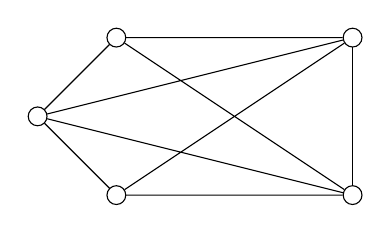
\begin{tikzpicture}[main_node/.style={circle,draw,inner sep=3pt], scale=0.8}]

    \node[main_node] (1) at (-2, 0) {};
    \node[main_node] (2) at (-1, 1)  {};
    \node[main_node] (3) at (-1,-1) {};
    \node[main_node] (4) at (2,1)  {};
    \node[main_node] (5) at (2, -1) {};
    \draw (2) -- (1) -- (3);
    \draw (4) -- (5);
    \draw (5) -- (1) -- (4) -- (2) -- (5) -- (3) -- (4);
\end{tikzpicture}
\caption{Unija (levo) in spoj (desno) grafov $K_{1,2}$ in $K_2$.}
\end{figure}

Za poljubno vozlišče $u$ definirajmo njegovo \emph{soseščino $N(u)$} kot vsa vozlišča $v \in V(G)$, da velja $(u,v) \in E(G)$. Soseščina je \emph{zaprta}, če vsebuje tudi vozlišče $u$, kar označimo z oznako $N[u]$. Za dve različni vozlišči $x$, $y$ rečemo, da imata \emph{skupno soseščino}, če velja $N(x) - \{x,y\} = N(y) - \{x,y\}$. Podobno bomo z oznako $N(U)$ označevali unijo soseščin vseh vozlišč iz $U$, vendar brez množice $U$, to je $\bigcup_{u \in U}N(u) \setminus U$, prav tako pa bo $N[U]$ pomenila unijo zaprtih soseščin, torej $\bigcup_{u \in U}N[u]$. 

Nadalje definirajmo \emph{neodvisno množico} kot množico vozlišč, ki paroma niso sosedna, ter \emph{kliko} kot množico vozlišč, kjer so vsa vozlišča množice paroma sosedna. Hitro se da preveriti, da je množica $S\subseteq V(G)$ neodvisna množica v grafu $G$ natanko tedaj, ko je $S$ klika v $\overline{G}$. Pri uporabi termina klika ne bomo ločevali med množico vozlišč, ki inducirajo poln graf, ter induciranim polnim grafom. \emph{Klično število $\omega(G)$} je kardinalnost največje klike grafa $G$.

\emph{Dominantna množica}\index{dominantna množica} $D$ grafa $G$ je taka množica vozlišč $D \subseteq V(G)$, da za vsako vozlišče $v \in V(G) \setminus D$ obstaja takšno vozlišče $u \in D$, da $v$ leži v $N[u]$. \emph{Dominantno število $\gamma(G)$} \index{dominantno število} je kardinalnost najmanjše dominantne množice za graf $G$. Dominantno množico, katere kardinalnost je enaka dominantnemu številu grafa, imenujemo $\gamma$-množica.

%%%%%%%%%%%%%%%%%%%%%%%%%%%%%%%%%%%%%%%%%%%%%%%%%%%%%%%%%%%%%%%%%
%%%%%%%%%%%%%%%%%%%%%%%%%%%%%%%%%%%%%%%%%%%%%%%%%%%%%%%%%%%%%%%%%
%%%                       KOGRAFI                             %%%
%%%%%%%%%%%%%%%%%%%%%%%%%%%%%%%%%%%%%%%%%%%%%%%%%%%%%%%%%%%%%%%%%
%%%%%%%%%%%%%%%%%%%%%%%%%%%%%%%%%%%%%%%%%%%%%%%%%%%%%%%%%%%%%%%%%
\section{Karakterizacije kografov}
V začetku poglavja si bomo ogledali definicijo in nekaj lastnosti kografov. Podali bomo reprezentacijo kografov s kodrevesi in pojasnili njihov algoritmični pomen. Kasneje bomo navedli in dokazali izrek o karakterizacijah kografov in pri tem v večini sledili članku~\cite{corneil1981complement}. Zadnje podpoglavje bo namenjeno algoritmičnim in drugim lastnostim kografov. Pokazali bomo, da kografi spadajo v razred popolnih grafov ter predstavili aplikacijo tega dejstva na področju barvanja grafov. Za konec bomo navedli nekaj algoritmov, ki zaradi posebne strukture kodreves delujejo v linearnem času, in motivirali naslednje poglavje o varnostni dominaciji, za katero se izkaže, da je na kografih rešljiva v linearnem času.
\subsection{Kografi in kodrevesa}\label{kografiInKodrevesa}
Sprva rekurzivno definirajmo kograf.
\begin{definicija}
\index{kograf}\emph{Kograf} je rekurzivno definiran na sledeč način:
\begin{enumerate}[label=($\roman*$)]
\item $K_1$ je kograf.
\item Če so $G_1, \dots, G_k$ kografi, je tudi njihova unija $G_1 \cup \cdots \cup G_k$ kograf.
\item Če je $G$ kograf, je tudi njegov komplement $\overline{G}$ kograf.
\end{enumerate}
\end{definicija}
Iz definicije je razvidno, da vsak kograf s končnim številom vozlišč $n$ lahko pridobimo z zaporedjem operacij unije in komplementa. Za potrebe te naloge in algoritmičnih pristopov se bomo osredotočili le na končne grafe.

\begin{primer}
Slika~\ref{primerMajhnihKografov} prikazuje primere kografov na enem, dveh ali treh vozliščih, kjer opazujemo strukturo grafa do izomorfizma natančno.

\begin{figure}[h!]
\centering

\begin{tikzpicture}[main_node/.style={circle,minimum size = 0.7cm,draw,inner sep=5pt, scale=0.6}]
    \node[main_node] (1) at (0, 0) {};
\end{tikzpicture}
\hspace{60pt}
\begin{tikzpicture}[main_node/.style={circle,minimum size = 0.7cm,draw,inner sep=5pt, scale=0.5}]
    \node[main_node] (1) at (-0.7, 1) {};
    \node[main_node] (2) at (0.7, 1)  {};
    \node[main_node] (3) at (-0.7, -1) {};
    \node[main_node] (4) at (0.7, -1)  {};
    \draw (3) -- (4);
\end{tikzpicture}
\hspace{60pt}
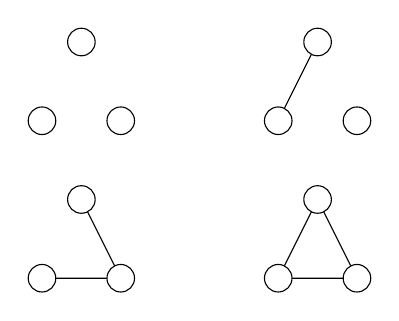
\begin{tikzpicture}[main_node/.style={circle,minimum size = 0.7cm,draw,inner sep=5pt, scale=0.5}]
    \node[main_node] (1) at (-1.5, 2) {};
    \node[main_node] (2) at (-2, 1)  {};
    \node[main_node] (3) at (-1, 1)  {};
    
    \node[main_node] (4) at (1.5, 2) {};
    \node[main_node] (5) at (2, 1)  {};
    \node[main_node] (6) at (1, 1)  {};
    
    \node[main_node] (7) at (-2, -1) {};
    \node[main_node] (8) at (-1, -1)  {};
    \node[main_node] (9) at (-1.5, 0)  {};
    
 	\node[main_node] (10) at (2, -1) {};
    \node[main_node] (11) at (1, -1)  {};
    \node[main_node] (12) at (1.5, 0)  {};
    
    \draw (4) -- (6);
    \draw (7) -- (8) -- (9);
    \draw (10) -- (11) -- (12) -- (10);
 
\end{tikzpicture}
\caption{Vsi možni grafi na enem (levo), dveh (sredina) in treh (desno) vozliščih so hkrati tudi kografi.} \label{primerMajhnihKografov}
\end{figure}
\begin{itemize}
\item Graf na enem vozlišču je po definiciji tudi kograf.
\item Graf na dveh vozliščih ima eno ali nobene povezave. Če ima povezavo, smo graf dobili s komplementom unije dveh vozlišč. Če povezave ni, je dobljen graf nepovezan in posledica unije dveh vozlišč. Iz tega sledi, da sta oba grafa na dveh vozliščih tudi kografa.
\item Graf na treh vozliščih ima lahko nič, eno, dve ali tri povezave. Graf z nič povezavami dobimo z unijo treh vozlišč. Graf z eno povezavo je posledica komplementne unije dveh vozlišč, nato pa jo z unijo združimo še s preostalim vozliščem. Graf z dvema povezavama je komplement prej opisanega grafa z eno povezavo, polni graf na treh vozliščih pa dobimo s komplementom unije vseh treh vozlišč. Iz tega sledi, da so vsi grafi na dveh vozliščih hkrati tudi kografi.
\end{itemize}
Opazimo, da se vzorec konča z grafi na štirih vozliščih, saj je pot dolžine štiri ($P_4$) najmanjši primer grafa, ki ni kograf. Ker je komplement $P_4$ prav tako $P_4$ ter je ni mogoče zapisati kot unijo manjših kografov, pot dolžine štiri ni kograf. V glavnem izreku~\ref{karakterizacija} tega poglavja se bomo tudi prepričali, da gre za edini kritičen graf strukture kografa.
\end{primer}

Končno število operacij unije in komplementa lahko ponazorimo z drevesom s korenom, ki ga imenujemo \index{kodrevo}\emph{kodrevo}; listi v drevesu so vozlišča grafa $G$, notranja vozlišča pa ustrezajo operaciji komplementarne unije, ki določa povezave posameznih vozlišč znotraj kografa. Primer postopka prikazuje slika~\ref{fig:kograf}. Kograf grafa $G$ označujemo z oznako $T_G$, oznaka $T_G(v)$ pa označuje induciran podgraf grafa $G$, ki je induciran z listi poddrevesa $T_G$ s korenom v vozlišču $v$.

\begin{figure}[h!]
\centering
\begin{tikzpicture}[]
\node (ena) at (0,0) {
\begin{tikzpicture}[main_node/.style={circle,minimum size = 0.9cm,draw,inner sep=5pt, scale=0.8}]
    \node[main_node] (1) at (0, 2) {$a$};
    \node[main_node] (2) at (1.5, 1.5)  {$b$};
    \node[main_node] (3) at (1.5, -1) {$c$};
    \node[main_node] (4) at (-1.5, -1)  {$d$};
    \node[main_node] (5) at (-1.5, 1.5) {$e$};
    \draw (1) -- (2) -- (3) -- (4) -- (5) -- (1);
    \draw (2) -- (4);
    \draw (3) -- (5);
\end{tikzpicture}};
\node (dva) at (-4, -4) {
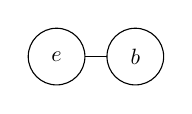
\begin{tikzpicture}[main_node/.style={circle,minimum size = 0.9cm,draw,inner sep=5pt, scale=0.8}]
    \node[main_node] (2) at (0.5, 2.5)  {$b$};
    \node[main_node] (5) at (-0.5, 2.5) {$e$};
    \draw (5) -- (2);
\end{tikzpicture}};
\node (pet) at (4, -4) {
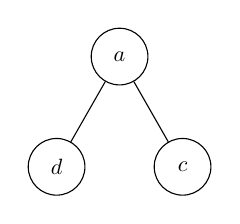
\begin{tikzpicture}[main_node/.style={circle,minimum size = 0.9cm,draw,inner sep=5pt, scale=0.8}]
    \node[main_node] (1) at (0, 0.5) {$a$};
    \node[main_node] (3) at (0.8, -0.9) {$c$};
    \node[main_node] (4) at (-0.8, -0.9)  {$d$};
    \draw (3) -- (1) -- (4);
\end{tikzpicture}};
\node (tri) at (-5, -6) {
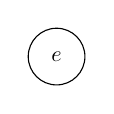
\begin{tikzpicture}[main_node/.style={circle,minimum size = 0.9cm,draw,inner sep=5pt, scale=0.8}]
    \node[main_node] (2) at (0, 0)  {$e$};
\end{tikzpicture}};
\node (stiri) at (-3, -6) {
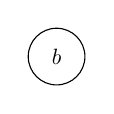
\begin{tikzpicture}[main_node/.style={circle,minimum size = 0.9cm,draw,inner sep=5pt, scale=0.8}]
    \node[main_node] (2) at (0, 0)  {$b$};
\end{tikzpicture}};
\node (sest) at (2, -6.5) {
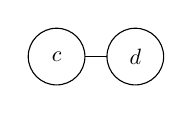
\begin{tikzpicture}[main_node/.style={circle,minimum size = 0.9cm,draw,inner sep=5pt, scale=0.8}]
    \node[main_node] (3) at (-0.5, 0) {$c$};
    \node[main_node] (4) at (0.5, 0)  {$d$};
    \draw (3) -- (4);
\end{tikzpicture}};
\node (sedem) at (6, -6.5) {
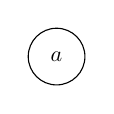
\begin{tikzpicture}[main_node/.style={circle,minimum size = 0.9cm,draw,inner sep=5pt, scale=0.8}]
    \node[main_node] (1) at (0, 0) {$a$};
\end{tikzpicture}};
\node (osem) at (1, -8.3) {
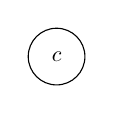
\begin{tikzpicture}[main_node/.style={circle,minimum size = 0.9cm,draw,inner sep=5pt, scale=0.8}]
    \node[main_node] (3) at (-0.7, 0) {$c$};
\end{tikzpicture}};
\node (devet) at (3, -8.3) {
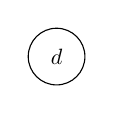
\begin{tikzpicture}[main_node/.style={circle,minimum size = 0.9cm,draw,inner sep=5pt, scale=0.8}]
    \node[main_node] (4) at (0.7, 0)  {$d$};
\end{tikzpicture}};
\path[->] (ena) edge node {} (dva);
\path[->] (dva) edge node {} (tri);
\path[->] (dva) edge node {} (stiri);
\path[->] (ena) edge node {} (pet);
\path[->] (pet) edge node {} (sest);
\path[->] (sest) edge node {} (osem);
\path[->] (sest) edge node {} (devet);
\path[->] (pet) edge node {} (sedem);
\end{tikzpicture}

\caption{Razčlemba kografa s postopkom komplementarne unije na povezanih komponentah. Zgoraj je kograf $G$, vsaka puščica pa predstavlja operacijo komplementarne unije. S pomočjo tega postopka je definirano \emph{kodrevo}, ponazoritev postopka v obliki drevesa. Kodrevo za zgornji graf je prikazano na sliki~\ref{fig:kodrevo}.} \label{fig:kograf}
\end{figure}

\begin{trditev}\label{kodrevoKograf}
Kodrevo za kograf $G$ je določeno enolično do izomorfizma natančno.
\end{trditev}

\begin{proof}
Naj bo $G$ povezan kograf (sicer obravnavamo vsako komponento posebej) z vsaj dvema vozliščema (sicer je kograf hkrati tudi kodrevo). Po definiciji mora biti $G$ komplement kografa, edina možnost za $\overline{G}$ pa je, da je unija manjših kografov. Za koren drevesa zato izberemo vozlišče, ki predstavlja operacijo komplementarne unije (oznaka $\overline{\cup}$), potomci tega drevesa pa bodo določeni glede na dobljene povezane komponente kografa $G$. Če je v izbrani povezani komponenti le eno vozlišče, je potomec kar list z oznako vozlišča; sicer je potomec kodrevo, ki ga dobimo, če postopek komplementarne unije rekurzivno ponavljamo na izbrani povezani komponenti. Ker je operacija komplementa ter razdelitev grafa na povezane komponente enolična do vrstnega reda povezanih komponent natančno, s takim algoritmičnim pristopom ustvarimo kodrevo, ki je enolično do izomorfizma natančno.
\end{proof}

Za lažje razumevanje strukture grafa lahko namesto operacije komplementarne unije $\overline{\cup}$ uporabimo operaciji unije $\cup$ in spoja $+$ na sledeč način: koren je vedno označen z $+$, potomci notranjega vozlišča z oznako $+$ imajo oznako $\cup$, potomci notranjega vozlišča z oznako $\cup$ pa imajo oznako $+$.

\begin{figure}[h!]
\centering
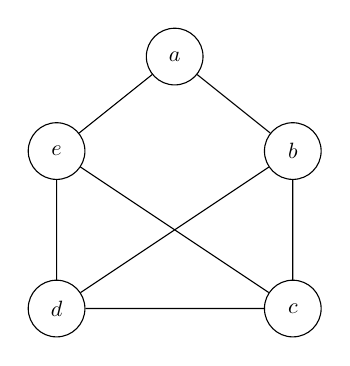
\begin{tikzpicture}[main_node/.style={circle,minimum size = 0.9cm,draw,inner sep=5pt, scale=0.8}]
    \node[main_node] (1) at (0, 4.2) {$a$};
    \node[main_node] (2) at (1.5, 3)  {$b$};
    \node[main_node] (3) at (1.5, 1) {$c$};
    \node[main_node] (4) at (-1.5, 1)  {$d$};
    \node[main_node] (5) at (-1.5, 3) {$e$};
    \draw (1) -- (2) -- (3) -- (4) -- (5) -- (1);
    \draw (2) -- (4);
    \draw (3) -- (5);
\end{tikzpicture}
\hspace{15pt}
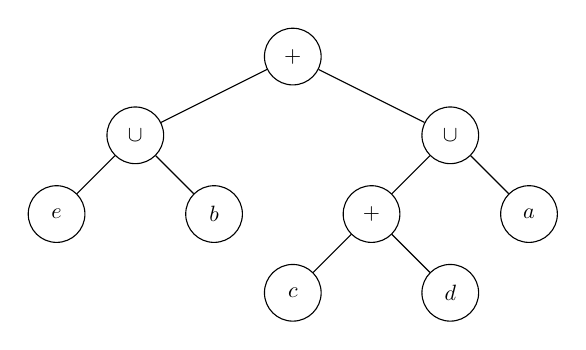
\begin{tikzpicture}[main_node/.style={circle,draw,inner sep=3pt,minimum size = 0.9cm, scale=0.8}]

	\node[main_node] (1) at (2, 0) {$d$};
    \node[main_node] (2) at (0, 0) {$c$};
    \node[main_node] (3) at (3, 1)  {$a$};
    \node[main_node] (4) at (-1, 1) {$b$};
    \node[main_node] (5) at (-3, 1)  {$e$};
    \node[main_node] (6) at (1, 1) {$+$};
    \node[main_node] (7) at (2, 2) {$\cup$};
    \node[main_node] (8) at (-2, 2)  {$\cup$};
   
    \node[main_node] (9) at (0, 3)  {$+$};
 
   
    \draw (9) -- (7) -- (6) -- (1);
    \draw (6) -- (2);
    \draw (7) -- (3);
    \draw (9) -- (8) -- (4);
    \draw (8) -- (5);
 
\end{tikzpicture}
\caption{Graf $G$ s slike~\ref{fig:kograf} (levo) in pripadajoče kodrevo (desno).} \label{fig:kodrevo}
\end{figure}

Hitro lahko preverimo, da zapisa predstavljata enake operacije na grafu. Če je dolžina poti od korena do izbranega notranjega vozlišča liha, smo operacijo komplementa uporabili v sodem številu korakov, kar pomeni, da smo podgrafa, ki ustrezata poddrevesu izbranega notranjega vozlišča, združili z unijo $\cup$. Če je ta dolžina soda in smo komplement uporabili na lihem številu korakov, smo unijo omenjenih podgrafov napravili na komplementu grafa, kar se na grafu kaže kot spoj $+$ dveh podgrafov. Ta zapis direktno poraja naslednjo posledico.



\begin{posledica} \label{povezanostVKodrevesu}
Naj bo $G$ kograf in $T_G$ njegovo kodrevo. S $P_x$ označimo najkrajšo pot v drevesu $T_G$ od vozlišča $x \in V(G)$ do korena drevesa. Za poljubni različni vozlišči $x, y$ v kografu $G$ velja, da sta sosedni natanko tedaj, ko je prvo skupno vozlišče od $P_x$ in $P_y$ (notranje) vozlišče z oznako $+$.
\end{posledica}
Opazimo tudi, da z globino drevesa določamo skupine v kografu, ki se v preostali graf vpenjajo na enak način. Na primer: naj bo $c$ notranje vozlišče z oznako $+$, $T_1,\dots, T_k$ pa poddrevesa vozlišča $c$. Vsak list poddrevesa $T_i$ je v kografu soseden vsakemu listu $T_j$, $i \neq j$; kako so povezani listi v poddrevesu med sabo, pa določajo nižje ležeča notranja vozlišča.


\begin{primer}
Iz definicije kografov sledi, da med njih spadajo polni in prazni grafi, prav tako pa tudi polni multipartitni grafi, med katere sodijo polni dvodelni in Turanovi grafi (slika~\ref{fig:primerKodrevesDruzineGrafov}).
\begin{figure}[h!]
\centering
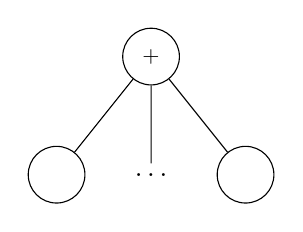
\begin{tikzpicture}[main_node/.style={circle,draw,inner sep=3pt,minimum size = 0.9cm, scale=0.8}]
	\node[main_node] (1) at (0,0) {$+$};
    \node[main_node] (2) at (-1.2, -1.5) {};
    \node[] (3) at (0, -1.5) {$\hdots$};
    \node[main_node] (4) at (1.2, -1.5) {};
    \draw (2) -- (1) -- (3);
    \draw (4) -- (1);
\end{tikzpicture}
\hspace{20pt}
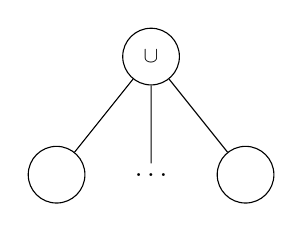
\begin{tikzpicture}[main_node/.style={circle,draw,inner sep=3pt,minimum size = 0.9cm, scale=0.8}]
	\node[main_node] (1) at (0,0) {$\cup$};
    \node[main_node] (2) at (-1.2, -1.5) {};
    \node[] (3) at (0, -1.5) {$\hdots$};
    \node[main_node] (4) at (1.2, -1.5) {};
    \draw (2) -- (1) -- (3);
    \draw (4) -- (1);
\end{tikzpicture}
\hspace{20pt}
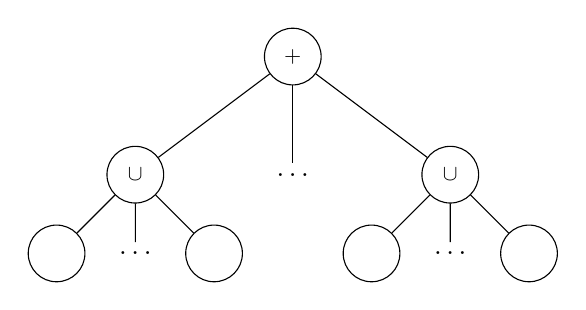
\begin{tikzpicture}[main_node/.style={circle,draw,inner sep=3pt,minimum size = 0.9cm, scale=0.8}]
	\node[main_node] (1) at (0,0) {$+$};
    \node[main_node] (2) at (-2, -1.5) {$\cup$};
    \node[] (3) at (0, -1.5) {$\hdots$};
    \node[main_node] (4) at (2, -1.5) {$\cup$};
    \node[main_node] (5) at (3, -2.5) {};
    \node[main_node] (6) at (1, -2.5) {};
    \node[] (7) at (2, -2.5) {$\hdots$};
    \node[main_node] (8) at (-3, -2.5) {};
    \node[main_node] (9) at (-1, -2.5) {};
    \node[] (10) at (-2, -2.5) {$\hdots$};
\draw (10) -- (2) -- (9);
\draw (8) -- (2) -- (1) -- (4) -- (7);
\draw (5) -- (4) -- (6);
\draw (1) -- (3);
\end{tikzpicture}
\caption{Primer kodrevesa za polni graf (levo), prazni graf (sredina) in polni multipartitni graf (desno).} \label{fig:primerKodrevesDruzineGrafov}
\end{figure}
\end{primer}

Navedimo še dve precej očitni, a pomembni lastnosti strukture kodrevesa.

\begin{opomba}\label{Observation 5}
Naj bo $T_G$ kodrevo za kograf $G$ in $c$ notranje vozlišče kodrevesa z oznako $\cup$. Tedaj velja, da je vsak potomec vozlišča $c$ bodisi list bodisi vozlišče z oznako $+$. Še več, graf $T_G(c)$ je nepovezan graf.
\end{opomba}
\begin{opomba}\label{Observation 6}
Naj bo $T_G$ kodrevo za kograf $G$ in $c$ notranje vozlišče kodrevesa z oznako $+$. Tedaj velja, da je vsak potomec vozlišča $c$ bodisi list bodisi vozlišče z oznako $\cup$. Še več, graf $T_G(c)$ je poln graf natanko tedaj, ko je vsak potomec vozlišča $c$ list.
\end{opomba}

Da je določen graf kograf, lahko po trditvi~\ref{kodrevoKograf} potrdimo ali ovržemo s konstrukcijo kodrevesa. Leta 1978 je L. Stewart v \cite{stewart1978cographs} predstavil algoritem za prepoznavanje kografov in konstrukcijo kodreves, ki deluje v $O(n(G)^2)$ času. V letih 1981--1984 so bili študirani algoritmi za barvanja kografov, prepoznavanje izomorfizmov med kografi, iskanje klik in dominantnih množic ter Hamiltonovih ciklov \cite{corneil1981complement}, \cite{corneil1984clustering}, \cite{corneil1984cographs}, ki imajo na kodrevesih linearno časovno zahtevnost in ki jih bomo podrobneje pogledali v poglavju~\ref{sec:algoritmicneInDrugeLastnosti}, zato se je porajalo vprašanje, če je mogoče kodrevo konstruirati v linearnem času. Že leta 1985 so D. G. Corneil, Y. Perl in L. Stewart objavili članek~\cite{corneil1985linear}, ki opisuje tak algoritem. Osnova algoritma je izrek \cite[Theorem 1]{corneil1985linear}, ki s posebnim označevanjem vozlišč nudi pogoj, kdaj kograf ob dodajanju novega vozlišča ohrani lastnosti kografa. Algoritem \cite[Algorithm Cograph-recognition]{corneil1985linear} kot vhod sprejme poljubni vrstni red vozlišč grafa $G$ ter prvi dve vozlišči poveže v kodrevo z vozliščem, ki mu priredi oznako glede na obstoj povezave med vozliščema. Nato na vsaki iteraciji pokliče metodo označevanja vozlišč kodrevesa ter glede na izrek \cite[Theorem 1]{corneil1985linear} določi, ali je novo pridobljeni podgraf prav tako kograf, na koncu pa s pomočjo označevanja kodrevesa umesti novo vozlišče v kodrevo.

\medskip
Izkaže se, da se mnogi algoritmični problemi na kografih lahko poenostavijo, če ima vsako notranje vozlišče kodrevesa največ dva potomca. Zato kot posebno obliko kodrevesa definirajmo \emph{binarno kodrevo} kot binarno drevo, ki ima za liste vozlišča grafa $G$, notranja vozlišča pa so operacije unije in spoja, s katerimi delujemo na grafih, induciranih z listi pripadajočih poddreves. Iz kodrevesa lahko binarno kodrevo napravimo s sprehodom po kodrevesu v vrstnem redu BFS algoritma z začetkom v korenu drevesa. Pri tem vsako vozlišče $c$, ki ima $n$ potomcev, kjer je $n > 2$, zamenjamo z $n-1$ dolgo potjo enako označenih notranjih vozlišč (prvo vozlišče poti je sosedno staršu vozlišča $c$), vsakemu vozlišču poti pa kot potomca določimo enega izmed potomcev vozlišča $c$ (z izjemo zadnjega vozlišča poti, ki mu priredimo dva potomca), glej primer~\ref{primerBinarno}. S tem ohranimo relacije znotraj kografa, saj se najkrajše poti dveh poljubnih vozlišč v binarnem kodrevesu prvič sekata v vozlišču z enako oznako, kot je bila v običajnem kodrevesu, hkrati pa dosežemo, da ima vsako vozlišče največ dva potomca. Postopek je reverzibilen, zato iz binarnega kodrevesa dobimo običajno kodrevo z zamenjavo morebitnih poti notranjih vozlišč z enakimi oznakami. Take poti zamenjamo z enim vozliščem z enako oznako, katerega potomci so vozlišča, ki so bili potomci katerega izmed vozlišč v omenjeni poti.

Opazimo, da s spremembo kodrevesa v binarno kodrevo ne ohranimo lastnosti, opisanih v opombah~\ref{Observation 5} in \ref{Observation 6}. Ker se z obema postopkoma sprehodimo čez graf le enkrat, je časovna zahtevnost linearna.

\begin{primer}\label{primerBinarno}
Na sliki \ref{fig:primerBinarno} je primer kografa, njegovega kodrevesa in binarnega kodrevesa. Opazimo, da ima notranje vozlišče kodrevesa z oznako $\cup$ štiri potomce. Z zgoraj opisanim postopkom vozlišče zamenjamo za pot dolžine tri, posamezne potomce vozlišče $\cup$ pa povežemo na posamezna vozlišča novo dodane poti. Dobimo binarno kodrevo, ki je na sliki spodaj desno.
\begin{figure}[h!]
    \centering
    \begin{tikzpicture}[]
    \node (ena) at (0.5,4.5) {
        \begin{tikzpicture}[main_node/.style={circle,minimum size = 0.9cm,draw,inner sep=5pt, scale=0.8}]
        \node[main_node] (1) at (0, 3.5) {$a$};
        \node[main_node] (2) at (1.2, 2.8)  {$b$};
        \node[main_node] (3) at (1.2, 1) {$c$};
        \node[main_node] (4) at (-1.2, 1)  {$d$};
        \node[main_node] (5) at (-1.2, 2.8) {$e$};
        \draw (1) -- (2) -- (3) -- (4) -- (5) -- (1);
        \draw (2) -- (4);
        \draw (3) -- (5);
        \end{tikzpicture}};
    \node (dva) at (-3.5,0) {
        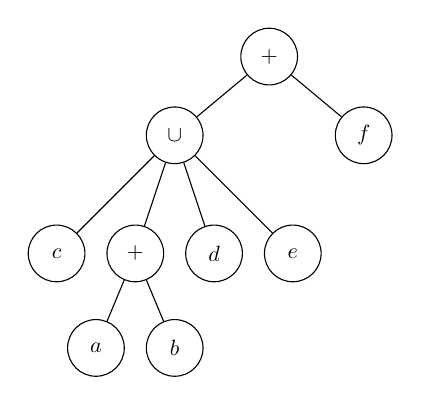
\begin{tikzpicture}[main_node/.style={circle,draw,inner sep=3pt,minimum size = 0.9cm, scale=0.8}]
	    \node[main_node] (1) at (1.2,0) {$+$};
        \node[main_node] (2) at (0,-1) {$\cup$};
	    \node[main_node] (3) at (2.4,-1) {$f$};
	    \node[main_node] (4) at (-0.5,-2.5) {$+$};
	    \node[main_node] (5) at (0.5,-2.5) {$d$};
	    \node[main_node] (6) at (-1.5,-2.5) {$c$};
	    \node[main_node] (7) at (1.5,-2.5) {$e$};
	    \node[main_node] (8) at (-1,-3.7) {$a$};
	    \node[main_node] (9) at (0,-3.7) {$b$};
	    
	    \draw (3) -- (1) -- (2) -- (6);
	    \draw (7) -- (2) -- (5);
	    \draw (9) -- (4) -- (8);
	    \draw (4) -- (2);
    \end{tikzpicture}};
    
    \node (tri) at (3.5,0) {
        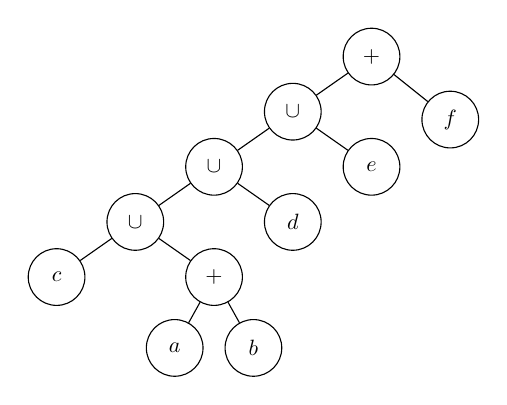
\begin{tikzpicture}[main_node/.style={circle,draw,inner sep=3pt,minimum size = 0.9cm, scale=0.8}]
	    \node[main_node] (1) at (1.5, 0) {$+$};
	    \node[main_node] (3) at (2.5,-0.8) {$f$};
	    \node[main_node] (4) at (-0.5,-2.8) {$+$};
	    \node[main_node] (5) at (0.5,-2.1) {$d$};
	    \node[main_node] (6) at (-2.5,-2.8) {$c$};
	    \node[main_node] (7) at (1.5,-1.4) {$e$};
	    \node[main_node] (8) at (-1,-3.7) {$a$};
	    \node[main_node] (9) at (0,-3.7) {$b$};
	    \node[main_node] (10) at (0.5, -0.7) {$\cup$};
	    \node[main_node] (11) at (-0.5, -1.4) {$\cup$};
	    \node[main_node] (12) at (-1.5, -2.1) {$\cup$};
	    
	    \draw (3) -- (1) -- (10) -- (11) -- (12) -- (6);
	    \draw (7) -- (10);
	    \draw (5) -- (11);
	    \draw (12) -- (4) -- (8);
	    \draw (9) -- (4);
        \end{tikzpicture}};
    \end{tikzpicture}
    \caption{Kograf (zgoraj), njegovo kodrevo (levo spodaj) in binarno kodrevo (desno spodaj).}
    \label{fig:primerBinarno}
\end{figure}
\end{primer}


\subsection{Karakterizacije kografov}
Pri preučevanju strukture in lastnosti grafov ter aplikaciji na drugih področjih znanosti (kografi se pojavljajo tudi v matematični biologiji na področju genomike, glej~\cite{hellmuth2013orthology}) je težko opaziti, da graf zadošča rekurzivni definiciji kografa, lažje pa je opaziti kakšno specifično lastnost. Ker so nekatere karakterizacije na videz nepovezane, so se lastnosti kografov raziskovale ločeno na različnih področjih. Karakterizacije so pod enotno definicijo združili D.~G.~Corneil, H.~Lerchs in L.~Stewart Burlingham leta 1981 v članku~\cite{corneil1981complement}, ki je povezal do tedaj poznano znanje tega področja z drugimi grafovskimi lastnostmi ter nam bo služil kot osnova tega podpoglavja.

Za dokaz glavnega izreka uporabimo trditev, ki dokazuje dednost lastnosti biti kograf.

\begin{trditev} \label{podgrafKografaJeKograf}
Vsak induciran podgraf kografa je kograf.
\end{trditev}
\begin{proof}
Za grafe velikosti 1, 2 in 3 je trditev očitna, saj so njihovi edini inducirani podgrafi velikosti 1 ali 2, zanje pa smo že v primeru~\ref{primerMajhnihKografov} pokazali, da so vsi grafi hkrati tudi kografi.

Oglejmo si sedaj graf $G$ z vsaj 4 vozlišči. Induciran podgraf dobimo z odstranjevanjem nekaterih vozlišč, zato je dovolj, če trditev dokažemo za graf $G - y$, kjer je $y$ poljubno vozlišče. Ker vsakemu kografu ustreza neko enolično določeno kodrevo, je za dokaz trditve dovolj, da poiščemo kodrevo, ki ustreza grafu $G - y$.

Naj bo $T = T_G$ kodrevo grafa $G$ in $x$ starš vozlišča $y$. Možna sta dva primera:
\begin{enumerate}[label=($\roman*$)]
\item Vozlišče $x$ ima več kot dva potomca (slika~\ref{fig:podgrafkografaJeKograf1}). Iz drevesa $T$ odstranimo vozlišče $y$, dobljeno drevo $T - y$ ustreza kodrevesu za graf $G-y$.

\begin{figure}[h!]
\centering
\begin{tikzpicture}[scale = 0.8]
\node[] (ena) at (-3,0) {
\begin{tikzpicture}[main_node/.style={circle,draw,inner sep=3pt,minimum size = 0.9cm, scale=0.8}]
	\node[] (5) at (1.2,1.2) {\reflectbox{$\ddots$}};
	\node[main_node] (1) at (0,0) {$x$};
    \node[main_node] (2) at (-2, -1.5) {$y$};
    \node[main_node] (3) at (0, -1.5)  {$y'$};
    \node[main_node] (4) at (2, -1.5) {$y''$};
	\node[] (6) at (0,-2.8) {$\vdots$};
	\node[] (7) at (2,-2.8) {$\vdots$};
    \draw (5) -- (1) -- (2);
    \draw (1) -- (3) -- (6);
    \draw (1) -- (4) -- (7);
\end{tikzpicture}};

\node[] (dva) at (0,0) {$\longrightarrow$};

\node[] (dva) at (3,0) {
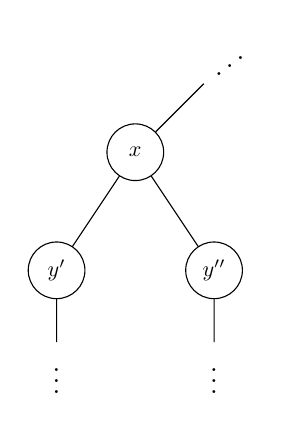
\begin{tikzpicture}[main_node/.style={circle,draw,inner sep=3pt,minimum size = 0.9cm, scale=0.8}]
	\node[] (5) at (1.2,1.2) {\reflectbox{$\ddots$}};
	\node[main_node] (1) at (0,0) {$x$};
    \node[main_node] (3) at (-1, -1.5)  {$y'$};
    \node[main_node] (4) at (1, -1.5) {$y''$};
	\node[] (6) at (-1,-2.8) {$\vdots$};
	\node[] (7) at (1,-2.8) {$\vdots$};
    \draw (5) -- (1);
    \draw (1) -- (3) -- (6);
    \draw (1) -- (4) -- (7);
\end{tikzpicture}};
\end{tikzpicture}
\caption{Primer iz dokaza leme~\ref{podgrafKografaJeKograf}, ko ima $x$ več kot dva potomca.} \label{fig:podgrafkografaJeKograf1}
\end{figure}

\item Vozlišče $x$ ima dva potomca, vozlišči $y$ in $z$ (slika~\ref{fig:podgrafkografaJeKograf2}). Poddrevo kodrevesa $T$ s korenom v $x$ vpliva le na to, kako so v grafu $G$ med seboj povezani elementi, ki se nahajajo v listih tega poddrevesa. Na poddrevo lahko torej gledamo kot na induciran podgraf na nekaterih vozliščih, v kograf pa so vpeti vsi na enak način---kot unija oziroma kot spoj, kar je odvisno od starša vozlišča $x$.

Če je $z$ prav tako list, iz drevesa odstranimo $x$, $z$ pa povežemo s staršem vozlišča $x$. V tem primeru je vozlišče $x$ določalo le, ali sta $y$ in $z$ med seboj povezana, povezave z ostalimi vozlišči pa so določala v drevesu višje ležeča vozlišča.
Če $z$ ni list, iz drevesa odstranimo $x$, $y$ in $z$, vse potomce vozlišča $z$ pa povežemo s staršem vozlišča $x$. Na ta način smo odstranili dve zaporedni notranji vozlišči in s tem ohranili tako povezave, ki jih v kografu določa poddrevo s korenom v $z$, kot tudi način vpenjanja v celotni kograf, ki ga določajo notranja vozlišča kodrevesa.


\begin{figure}[h!]
\centering
\begin{tikzpicture}[scale = 0.8]
\node[] (ena) at (-3,0) {
\begin{tikzpicture}[main_node/.style={circle,draw,inner sep=3pt,minimum size = 0.9cm, scale=0.8}]
	\node[] (8) at (2,2) {\reflectbox{$\ddots$}};
	\node[main_node] (5) at (1,1) {};
	\node[main_node] (1) at (0,0) {$x$};
    \node[main_node] (2) at (-1, -1.2) {$y$};
    \node[main_node] (4) at (1, -1.2) {$z$};
	\node[] (6) at (0,-2.5) {$\vdots$};
	\node[] (7) at (2,-2.5) {$\vdots$};
    \draw (8) -- (5) -- (1) -- (2);
    \draw (1) -- (4) -- (6);
    \draw (4) -- (7);
\end{tikzpicture}};
\node[] (dva) at (0,0) {$\longrightarrow$};
\node[] (dva) at (3,0) {
\begin{tikzpicture}[main_node/.style={circle,draw,inner sep=3pt,minimum size = 0.9cm, scale=0.8}]
	\node[] (8) at (2,2) {\reflectbox{$\ddots$}};
	\node[main_node] (5) at (1,1) {};
    \node[main_node] (4) at (1, -1.2) {$z$};
	\node[] (6) at (0,-2.5) {$\vdots$};
	\node[] (7) at (2,-2.5) {$\vdots$};
    \draw (8) -- (5) -- (4);
    \draw (4) -- (6);
    \draw (4) -- (7);
\end{tikzpicture}};
\end{tikzpicture}
\caption{Primer iz dokaza leme~\ref{podgrafKografaJeKograf}, ko ima $x$ natanko dva potomca.} \label{fig:podgrafkografaJeKograf2}
\end{figure}



\end{enumerate}
Ker smo v obeh primerih z brisanjem enega lista kodrevesa dobili novo kodrevo, sledi, da je tudi $G - y$ kograf.
\end{proof}

Trditev nam ponuja možnost, da lastnosti in karakterizacije kografov obravnavamo le na delu kografa, kar je velika prednost pri algoritmičnih pristopih h obravnavanju problemov. Zaradi te lastnosti večina algoritmov lahko deluje na način \textit{deli in vladaj}, kjer algoritem izvajamo rekurzivno na majhnih lokalnih množicah, nato pa na ustrezen način rezultate združujemo v celoto.


\medskip
Preden navedemo izrek karakterizacij kografov, definirajmo še nekaj izrazov, ki jih bomo uporabljali v nadaljevanju.

\emph{Maksimalna} klika oziroma neodvisna množica je taka podmnožica vozlišč, da vanjo ni mogoče dodati novega vozlišča in pri tem ohraniti lastnost klike oziroma neodvisne množice. Množico maksimalnih klik oziroma maksimalnih neodvisnih množic za graf $G$ označimo z oznako $\mathit{C_G}$ oziroma $\mathit{K_G}$ (oznaka sledi iz angleškega izraza \emph{clique} oziroma \emph{kernel}). Za lažje izražanje vpeljimo tudi oznako $\mathit{C_G(x)}$ (oziroma $\mathit{C_G(\overline{x})}$), ki označuje množico maksimalnih klik, ki vsebujejo vozlišče $x$ (oziroma, ki ne vsebujejo vozlišča $x$). Enako lahko (ne)vsebovanost vozlišča $x$ izrazimo tudi za množico maksimalnih neodvisnih množic z oznako $\mathit{K_G(x)}$ (oziroma $\mathit{K_G(\overline{x})}$). Pravimo, da ima graf \emph{lastnost CK} \index{lastnost CK} natanko tedaj, ko je presek poljubne maksimalne klike in poljubne maksimalne neodvisne množice v grafu $G$ neprazen, to je $\forall C\in \mathit{C_G}, \forall K \in \mathit{K_G} :C \cap K \neq \emptyset$.

Dodajmo k definiciji še to, da je pogoj nepraznosti preseka enak pogoju, da je presek vsebuje eno vozlišče; če bi vsaj dva elementa ležala tako v maksimalni kliki kot tudi v maksimalni neodvisni množici, bi morala biti povezana (zaradi lastnosti klike) in hkrati nepovezana (zaradi lastnosti neodvisne množice), to pa vodi do protislovja.
\begin{izrek}\label{karakterizacija}
Naj bo $G$ graf. Naslednje trditve so ekvivalentne:
\begin{enumerate}[label=(\roman*)]
\item $G$ je kograf.
\item Vsak netrivialen induciran podgraf grafa $G$ ima vsaj en par vozlišč, ki imata skupno soseščino.
\item Vsak netrivialen induciran podgraf grafa $G$ ima lastnost $CK$.
\item Graf $G$ nima induciranega podgrafa $P_4$.
\item Komplement vsakega povezanega podgrafa z vsaj enim vozliščem grafa $G$ je nepovezan.
\end{enumerate}
\end{izrek}

\begin{proof}
Privzamemo, da je $G$ povezan (sicer obravnavamo vsako komponento posebej) ter da velja $n(G) > 3$ (saj so za grafe, manjše od 3, trditve očitne). 

\medskip
$(i) \Rightarrow (ii)$ Ker je vsak induciran podgraf kografa tudi sam kograf, je za implikacijo dovolj pokazati, da ima vsak kograf vsaj en par vozlišč s skupno soseščino. Naj bo $T$ kodrevo kografa $G$. Po posledici~\ref{povezanostVKodrevesu} sledi, da imata lista z istim staršem enako soseščino. Še več, če njun starš predstavlja operacijo spoja, imata lista skupno celo zaprto soseščino, saj sta povezana tudi med seboj. Po privzetku o velikosti grafa $n(G) > 3$ notranje vozlišče z vsaj dvema listoma zagotovo obstaja, zato implikacija sledi.

\medskip
$(ii) \Rightarrow (iii)$ Implikacijo trditve dokažimo z indukcijo na velikost podgrafa grafa $G$. Za bazo indukcije preverimo, da ima graf na enem vozlišču $x$ eno maksimalno kliko in eno maksimalno neodvisno množico---vozlišče $x$, kar ustreza lastnosti $CK$.

Privzemimo zdaj, da lastnost velja za vse podgrafe grafa $G$, ki so velikosti $p$, ter pokažimo, da imajo lastnost $CK$ tudi podgrafi velikosti $p+1$. Naj bo $H$ podgraf grafa $G$ velikosti $p+1$. Po točki $(ii)$ obstajata vozlišči $x$ in $y$ s skupno soseščino. Ker je $H - y$, označimo ga s $H'$, velikosti $p$, ima po indukcijski predpostavki lastnost $CK$, z njenimi maksimalnimi klikami in neodvisnimi množicami pa lahko izrazimo tiste iz podgrafa $H$.
Razdelimo problem na dva dela:
\begin{itemize}
\item Vozlišči $x$ in $y$ imata skupno soseščino, ki ni zaprta.

Vsaka maksimalna neodvisna množica v $H$, ki ne vsebuje vozlišča $x$, gotovo vsebuje kakšno vozlišče iz $N(x)$ (sicer smo v protislovju z maksimalnostjo), zato zaradi skupne soseščine ne vsebuje niti vozlišča $y$. Torej so vse take maksimalne neodvisne množice za graf $H$ vsebovane tudi v grafu $H'$. Po istem razmisleku vsaka maksimalna neodvisna množica v $H'$, ki vsebuje vozlišče $x$, postane maksimalna neodvisna množica v grafu $H$, če ji dodamo vozlišče $y$. Tako velja 
\begin{equation} \label{neodvisne_mnozice}
\mathit{K_H}(\overline{x}) = \mathit{K_{H'}}(\overline{x}),\hspace{15px}\mathit{K_H}(x) = \mathit{K_{H'}}(x) + y.
\end{equation}
Klike za razliko od neodvisnih množic razdelimo glede na vsebovanost vozlišča $y$. Vsaka maksimalna klika v $H$, ki ne vsebuje vozlišča $y$, je kar poljubna maksimalna klika v grafu $H'$. Če maksimalna klika v $H$ vsebuje vozlišče $y$, pa ga v podgrafu $H'$ nadomestimo z vozliščem $x$, saj je $N(x)$ vsa vsebovana v kliki, torej po maksimalnosti sledi, da mora tudi $x$ ležati v kliki. Tako velja
\begin{equation} \label{klike}
\mathit{C_H}(\overline{y}) = \mathit{C_{H'}},\hspace{15px}\mathit{C_H}(y) = \mathit{C_{H'}}(y) + y - x.
\end{equation}
S pomočjo zgornjih zvez in indukcijske predpostavke lahko hitro preverimo, da za poljubno $C\in \mathit{C_H} = \mathit{C_H}(y) \cup \mathit{C_H}(\overline{y})$ ter $K\in \mathit{K_H} = \mathit{K_H}(x) \cup \mathit{K_H}(\overline{x})$ velja $|C \cap K | = 1$; na primer: naj bo $C\in \mathit{C_H}(\overline{y})$ ter $K\in \mathit{K_H}(x)$. Tedaj zaradi zvez~\ref{neodvisne_mnozice},~\ref{klike} velja
$$|C \cap K | = |C' \cap (K' + y)|, $$
kjer je $C'\in \mathit{C_H'}$ ter $K' = K - {y}, K \in \mathit{K_H'}$. Po indukcijski predpostavki za podgrafe velikosti $p$ velja $|C' \cap K'| = 1$. Enako preverimo tudi za preostale tri kombinacije ($C\in \mathit{C_H}(y)$ ter $K\in \mathit{K_H}(x)$; $C\in \mathit{C_H}(y)$ ter $K\in \mathit{K_H}(\overline{x})$, $C\in \mathit{C_H}(\overline{y})$ ter $K\in \mathit{K_H}(\overline{x})$). Implikacija sledi.
\item Vozlišči $x$ in $y$ imata skupno zaprto soseščino.

Postopamo enako kot v prejšnjem primeru, le da tokrat maksimalne klike delimo glede na vsebovanost vozlišča $x$, neodvisne množice pa glede na vsebovanost vozlišča $y$. Po enakem razmisleku kot zgoraj dobimo štiri zveze za maksimalne klike/neodvisne množice v podgrafu $H$ in podgrafu $H'$:
\begin{align*}
\mathit{C_H}(\overline{x}) &= \mathit{C_{H'}}(\overline{x}),\hspace{15px}\mathit{C_H}(x) = \mathit{C_{H'}}(x) + y, \\
\mathit{K_H}(\overline{y}) &= \mathit{K_{H'}},\hspace{15px}\mathit{K_H}(y) = \mathit{K_{H'}}(y) + y - x.
\end{align*}
Na enak način preverimo, da za vse štiri kombinacije maksimalnih klik in neodvisnih množic sledi, da ima podgraf lastnost $CK$.
\end{itemize} 

\medskip
$(iii) \Rightarrow (iv)$ Po točki $(iii)$ ima vsak podgraf grafa $G$ lastnost $CK$, vendar ga pot dolžine štiri nima; če vozlišča poti označimo z $x, y, z, w$, sta vozlišči $x$ in $w$ maksimalna neodvisna množica, $y$ in $z$ pa maksimalna klika, presek pa je prazen.

\medskip
$(iv) \Rightarrow (v)$ Implikacijo dokažimo kot v članku \cite{seinsche1974property} tako, da negiramo obratno implikacijo: recimo, da obstaja podgraf z vsaj enim vozliščem povezanega grafa $G$, ki je tudi povezan, in pokažimo, da v njem najdemo induciran podgraf $P_4$.

\medskip
Recimo, da je $X\subseteq V(G)$ po kardinalnosti najmanjša taka množica, da je povezan tako z njo induciran podgraf $G[X]$ kot tudi njegov komplement $\overline{G[X]}$. Naj bo $x_1$ poljubno vozlišče množice $X$. Tedaj velja, da en od $G[X - \{x_1\}]$ ali $\overline{G[X - \{x_1\}]}$ ni povezan, sicer bi bili v protislovju z minimalnostjo. Brez škode za splošnost recimo, da $G[X - \{x_1\}]$ ni povezan. Ker sta $\overline{G[X]}$ in $\overline{G[X - \{x_1\}]}$ povezana, vozlišče $x_1$ ni most v $\overline{G[X]}$, zato obstaja vozlišče $x_2 \in X \setminus \{x_1\}$, ki je v $\overline{G[X]}$ soseden $x_1$. Ker $G[X \setminus \{x_1\}]$ ni povezan, ima vsaj dve komponenti za povezanost. Naj bo $X'$ množica vozlišč tiste komponente $G[X \setminus \{x_1\}]$, ki vsebuje vozlišče $x_2$ (prikazano na sliki~\ref{fig:graf4->5}). Množici $X \setminus (\{x_1\} \cup X')$ in $X'$ sta torej obe neprazni množici, med posameznimi vozlišči iz ene in druge množice pa ni poti. Ker je $G[X]$ povezan, obstajata vozlišči $x_3 \in X'$ in $x_4 \in X \setminus (\{x_1\} \cup X')$, ki sta sosedna $x_1$.
\begin{figure}[h]
\centering
\begin{tikzpicture}[main_node/.style={circle,draw,minimum size=2em,inner sep=1, scale=0.9}]
\usetikzlibrary{shapes}

    \node[main_node] (1) at (0,0) {$x_1$};
    \node[main_node] (2) at (0,-3.2) {$x_4$};
    \node[main_node] (3) at (3,0) {$x_3$};
    \node[main_node] (4) at (3,2.7) {$x_2$};
    \node[] (5) at (2.4,1.7) {};
    \node[] (6) at (3.6,1.7) {};
    \node[] (7) at (2.4,1) {};
    \node[] (8) at (3.6,1) {};
    
    \node[] (9) at (2,1.9) {};
    \node[] (10) at (4,1.9) {};
    \node[] (11) at (2,0.8) {};
    \node[] (12) at (4,0.8) {};
    
    \node[] (13) at (1,-2) {};
    \node[] (14) at (-1,-2) {};
    \node[] (15) at (-1.9,0.8) {};
    \node[] (16) at (-1.75,0) {};
    \node[] (17) at (-1.9,-0.8) {};
    \node[] (18) at (1.9,0.8) {};
    \node[] (20) at (1.9,-0.8) {};
    
     \node[] (21) at (5,4.1) {$X'$};
    \node[] (22) at (4.6,2) {$S$};
    \node[] (23) at (4.7,-0.6) {$S'$};
  

    \draw[densely dotted] (3,0) ellipse (1.6 and 1.2);
    \draw[densely dotted] (3,2.7) ellipse (1.6 and 1.2);
    \draw[densely dotted] (0, -3.2) ellipse (1.7 and 1.6);
    \draw[densely dotted] (-3, 0) ellipse (1.4 and 1.7);
    \draw[densely dotted] (3, 1.3) ellipse (2.6 and 3.2);
    
    \draw (5) --(7);
    \draw (6) -- (8);
    \draw (9) --(11);
    \draw (10) -- (12);
    
    \draw (13) -- (1) -- (14);
    \draw (15) -- (1) -- (16);
    \draw (17) -- (1);
    
    \draw (18) -- (1) -- (20);
    
    \draw (2) -- (1) -- (3);
    \draw (4) -- (3);


\end{tikzpicture}
\caption[Razdelitev grafa $G$ v dokazu 4 $\Rightarrow$ 5]{Razdelitev grafa v dokazu izreka~\ref{karakterizacija}, implikacija $(iv) \Rightarrow (v)$. Posamezne elipse (levo, spodaj in $X'$) so komponente za povezanost grafa $G[X - \{x_1\}]$. To pomeni, da obstajajo nekatere povezave med vozlišči znotraj komponente in vozliščem $x_1$, ne pa tudi med vozlišči iz različnih komponent.}
  \label{fig:graf4->5}
\end{figure}

Naj bo $S \subseteq X'$ podmnožica vozlišč, ki so sosedna $x_1$ v $\overline{G}$ in $S' \subseteq X \setminus (\{x_1\} \cup X')$, ki so sosedna $x_1$ v $\overline{G}$. Vemo, da $x_2 \in S$ in $x_3 \in S'$, zato $S, S \neq \emptyset$. Ker je $G[X]$ povezan, mora obstajati povezava med nekim vozliščem $x_2' \in S$ in $x_3' \in S'$. Imamo torej vozlišča $x_4$, $x_1$, $x_3'$ in $x_2'$, med katerimi imamo le povezave $x_4x_1$, $x_1x_3'$ in $x_3'x_2'$, kar pomeni, da je induciran graf na teh vozliščih izomorfen $P_4$. Prav tako v grafu $\overline{G[X]}$ opazimo induciran podgraf $P_4$ na vozliščih $x_1$, $x_2'$, $x_4$ in $x_3'$. Tako kot $G$ kot tudi $\overline{G}$ vsebujeta $P_4$ kot induciran podgraf. Implikacija sledi.

\medskip
$(v) \Rightarrow (i)$ Sprva se prepričajmo, da v primeru, ko $G$ premore lastnost iz alineje~$(v)$, ima to lastnost tudi $\overline{G}$. Recimo, da to ni res. Naj velja, da je komplement vsakega povezanega podgrafa grafa $G$ nepovezan (lastnost $(v)$), vendar naj bo $H$ tak povezan podgraf grafa $\overline{G}$, da je povezan tudi njegov komplement $\overline{H}$. Ker je hkrati $\overline{H}$ podgraf grafa $G$ ter je povezan, mora biti $H$ (komplement povezanega podgrafa $\overline{H}$) nepovezan, kar nas pripelje do protislovja.

\medskip
Dokažimo sedaj implikacijo s pomočjo indukcije na velikost grafa. Za grafe velikosti 3 je implikacija izpolnjena na prazno, saj so vsi taki majhni grafi hkrati tudi kografi. Zato dokažimo, da implikacija velja za grafe velikosti $n$, če predpostavimo, da velja za vse manjše. Ker sta lastnost~$(v)$ in lastnost \textit{biti kograf} neobčutljiva na operacijo komplementa, za implikacijo vzemimo tisti graf izmed $G$ in $\overline{G}$, ki je nepovezan. Ker je vsaka povezana komponenta tega grafa tudi podgraf manjše velikosti, po indukcijski predpostavki velja, da je tudi kograf.\end{proof}

\begin{opomba}
Rezultat trditve~\ref{podgrafKografaJeKograf}, da je vsak induciran podgraf kografa tudi sam kograf, smo uporabili za dokaz $(i) \Rightarrow (ii)$. Hitro se prepričamo, da trditev lahko izpeljemo tudi kot posledico zadnjega izreka; graf $G$ je kograf natanko tedaj, ko velja eden od pogojev $(ii)$--$(v)$, kar je natanko takrat, ko te pogoji veljajo tudi za vsak induciran podgraf grafa $G$.
\end{opomba}

\subsection{Algoritmične in druge lastnosti kografov}\label{sec:algoritmicneInDrugeLastnosti}
V tem poglavju bomo kografe povezali z nekaterimi večjimi družinami grafov. Zaradi strukture kografa in reprezentacije s kodrevesom se izkaže, da so določene lastnosti, ki so na poljubnih grafih težko izračunljive, na kografih izračunljive v linearnem času.

Zanimiva lastnost, ki kografe posledično uvršča v skupino popolnih grafov,  je popolna urejenost (vsak graf s popolno urejenostjo je popoln graf~\cite{maffray2003coloration}). To pomeni, da vozlišča grafa $G$ lahko uredimo na tak način, da požrešni algoritem barvanja, zagnan na seznamu tako urejenih vozlišč, vsak podgraf $H$ grafa $G$ pobarva optimalno---število porabljenih barv je enaka kromatičnemu številu $\chi(G)$. Še več, za kografe bomo pokazali, da vsaka ureditev njegovih vozlišč ustreza popolni urejenosti, kar pomeni, da je graf, pobarvan s požrešnim algoritmom, vedno pobarvan optimalno.

\medskip
Sprva se spomnimo, da za graf $G$ definiramo $k$-barvanje grafa kot surjekcijo $c: V(G) \rightarrow \{0, 1, ..., k-1\}$ tako, da velja $$uv \in E(G) \Rightarrow c(u) \neq c(v).$$ Najmanjši $k$, za katerega obstaja $k$-barvanje grafa $G$, je kromatično število $\chi(G)$ grafa $G$. Kadar je kromatično število $\chi(G)$ enako kličnemu številu $\omega(G)$, pravimo, da je graf \emph{popoln}.  \index{popoln graf}

\medskip
Nadalje definirajmo \emph{Grundyjevo} $k$-barvanje grafa $G$ \index{Grundyjevo k-barvanje}kot $k$-barvanje, kjer za vozlišče, pobarvano z barvo $i$, velja, da je sosedno nekemu vozlišču z barvo $j$ za vsak $j < i \leq k$. Grundyjevo barvanje tako ustreza barvanju, ki ga dobimo kot rezultat požrešnega barvanja grafa $G$, kjer vsako novo vozlišče v zaporedju  pobarvamo z najmanjšo možno barvo, da je barvanje še pravilno. \emph{Grundyjevo število $\mu(G)$} je maksimalno število $k$, da za graf $G$ obstaja Grundyjevo $k$-barvanje grafa $G$. Število $\mu$ si torej lahko predstavljamo kot najmanj optimalno barvanje grafa s požrešnim algoritmom.

Iz definicije in spodnje meje za kromatično število hitro sledi povezava med kličnim številom $\omega(G)$, kromatičnim številom $\chi(G)$ in Grundyjevim številom $\mu(G)$ za graf $G$: $$\omega(G) \leq \chi(G) \leq \mu(G).$$ Za poljubni lastnosti $\alpha, \beta \in \{\omega, \chi, \mu\}$ pravimo, da je graf $G$ \emph{$\alpha\beta$-popoln}, če za vsak induciran podgraf $H$ grafa $G$ velja $\alpha(H) = \beta(H)$. V primeru $\omega\chi$-popolnega grafa opazimo, da notacija sovpada s klasično definicijo popolnega grafa, zato se držimo kar običajnega poimenovanja.

Leta 1976 sta C.~A.~Christen in S.~M.~Selkow izdala članek~\cite{christen1979some}, kjer sta preučevala karakterizacije popolnih grafov. Dokazala sta povezavo med $\omega\mu$-popolnimi, $\chi\mu$-popolnimi grafi in grafi brez induciranega podgrafa $P_4$. Domneva, da popolni grafi ($\omega\chi$-popolni grafi) ustrezajo grafom brez induciranega lihega cikla velikosti najmanj pet ali njegovega komplementa, pa je ostala odprta do leta 2006, ko je bila potrjena in dokazana v članku~\cite{chudnovsky2006strong}. 

Karakterizirajmo sedaj $\chi\mu$-popolne grafe---grafe, pri katerih požrešni algoritem barvanja vedno  uporabi optimalno število barv. Najmanjši graf $G$, za katerega velja $\mu(G) < \chi(G)$, je $P_4$, presenetljivo pa je dejstvo, da je to tudi edini podgraf, ki se izključuje z lastnostjo $\chi\mu$-popolnosti.

\begin{izrek}\label{grundyjevaKarakterizacija}
Za poljuben graf $G$ so naslednje trditve ekvivalentne:
\begin{enumerate}[label=(\roman*)]
\item $G$ je $\omega\mu$-popoln.
\item $G$ je $\chi\mu$-popoln.
\item $G$ ne vsebuje induciranega podgrafa poti dolžine 4.
\end{enumerate}
\end{izrek}

\begin{proof} $(i) \Rightarrow (ii)$ Implikacija je trivialna, saj velja $\omega(G) \leq \chi(G) \leq \mu(G)$, torej iz $\omega(H) = \mu(H)$ za vsak induciran podgraf $H$ grafa $G$ sledi $\chi(H) = \mu(H)$.

\medskip
$(ii) \Rightarrow (iii)$ Implikacijo dokažimo s protislovjem. Naj bo $P_4$ induciran podgraf grafa $G$. Zanj velja $\chi(P_4)=2$, vendar je $\mu(P_4) = 3$, zato graf $G$ ne more biti $\chi\mu$-popoln graf.

\medskip
$(iii) \Rightarrow (i)$ Privzemimo, da $G$ ne vsebuje induciranega podgrafa $P_4$, hkrati pa naj bo $c$ poljubno Grundyjevo $\mu(G)$-barvanje grafa $G$. Implikacijo bomo dokazali s pomočjo indukcije na $m \leq \mu(G)$, kjer je $m$ velikost klike grafa $G$, ki je pobarvana z $m$ največjimi barvami barvanja $c$. Največja možna vrednost za $m$ je $\mu(G)$ (sicer smo v protislovju z maksimalnostjo števila $\mu(G)$), zato indukcija dokaže, da je graf $G$ $\omega\mu$-popoln.

Baza indukcije za $m=1$ očitno drži; če izberemo vozlišče v grafu z največjo barvo, je to induciran poln graf na enem vozlišču. Za indukcijski korak privzemimo, da obstaja klika velikosti $m-1$, ki vsebuje vozlišča $p_1, ..., p_{m-1}$, ki so pobarvana z med seboj različnimi $m-1$ največjimi barvami (to je z barvami $\mu(G)$, $\mu(G) - 1, \dots, \mu(G) - m + 1$). Za vsako vozlišče $p_i$, $i \in [m-1]$, označimo množico $S_i$ s tistimi vozlišči, ki so sosedni vozlišču $p_i$ in so v barvanju $c$ pobarvani z barvo $\mu(G) - m$. Ker je $c$ Grundyjevo barvanje, so $S_i$ zagotovo neprazne množice. Množice $S_i$ lahko uredimo z relacijo inkluzije --- če bi namreč obstajali vozlišči $u \in (S_i \setminus S_j)$ in $v\in (S_j \setminus S_i)$ za neka indeksa $i,j \in [m-1]$, bi graf $G$ vseboval inducirano pot na štirih vozliščih $u$, $p_i$, $p_j$ in $v$, kar je v protislovju s predpostavko. Zaradi relacije vsebovanosti in dejstva, da so vse množice neprazne, obstaja tak $k \in [m-1]$, da velja $$S_k = \bigcap_{1 \leq i < m} S_i.$$ Če poljubno vozlišče $p_m \in S_k$ dodamo v množico $p_1, \dots, p_{m-1}$, dobimo kliko velikosti $m$, ki je pobarvana z $m$ različnimi največjimi barvami barvanja $c$.

Ker smo z indukcijo pokazali, da v grafu $G$ obstaja klika velikosti $\mu(G)$, velja $\mu(G) = \omega(G)$ in implikacija sledi.\end{proof}

Eden od razlogov za preučevanje kografov je popolnost grafa. Leta 1961 je Berg domneval~\cite{berge1961coloring}, nato pa leta 1972 Lovász dokazal~\cite{lovasz1972characterisation}, da je komplement popolnega grafa popoln graf. Izkaže se, da je najmanjša družina grafov, ki so zaprti za komplement, ravno kografi, saj poleg komplementa dovoljujejo konstrukcijo kografov le s pomočjo unije. Verjetno je zaradi tega dejstva prišlo do sedaj uveljavljene definicije kografov, z naslednjo trditvijo pa se prepričajmo, da to dejstvo res drži.

\begin{trditev} Vsak kograf je popoln graf.
\end{trditev}
\begin{proof}
Glede na različne karakterizacije kografov lahko trditev dokažemo na različne načine:
\begin{itemize}
\item Kot posledico izreka~\ref{grundyjevaKarakterizacija}. Naj bo graf $G$ kograf. Po izreku~\ref{karakterizacija} sledi, da $G$ ne vsebuje induciranega grafa $P_4$, zato po izreku~\ref{grundyjevaKarakterizacija} sledita enakosti $\omega(H)=\mu(H)$ in $\chi(H)=\mu(H)$ za vsak induciran podgraf $H$ grafa $G$. Izrek sledi.

\item Kot posledico izreka o karakterizaciji popolnih grafov~\cite{chudnovsky2006strong}. Po rezultatu iz članka~\cite{chudnovsky2006strong} velja, da je graf popoln natanko tedaj, ko ne vsebuje induciranega lihega cikla $C_n$, $n \geq 5$, ali njegovega komplementa $\overline{C_n}$, $n \geq 5$. Za dokaz trditve je torej dovolj pokazati, da $G$ ne vsebuje induciranega lihega cikla ali njegovega komplementa, kar storimo s protislovjem. Recimo, da $G$ vsebuje lih cikel $C_n$, $n \geq 5$. Če iz tega cikla odstranimo eno vozlišče, dobimo induciran podgraf $P_{n-1}$, $n\geq 5$, kar pomeni, da graf vsebuje induciran podgraf $P_4$, kar zaradi izreka~\ref{karakterizacija} vodi do protislovja. Recimo sedaj, da vsebuje komplement lihega cikla $\overline{C_n}$. Po definiciji je komplement grafa tudi kograf, torej kograf $\overline{G}$ vsebuje lih cikel $C_n$, kar vodi v protislovje.

\item Kot posledico karakterizacije kografov iz izreka~\ref{karakterizacija} $(v)$. Dokažimo z indukcijo. Kograf na enem samem vozlišču je očitno popoln. Predpostavimo sedaj, da je $G$ poljuben kograf z več kot enim vozliščem. Zaradi dednosti lastnosti >>biti kograf<< lahko za indukcijski korak predpostavimo, da trditev velja za vse grafe, ki so po velikosti manjši od $G$. Po izreku~\ref{karakterizacija} $(v)$ je lastnost >>biti kograf<< enaka lastnosti, da je komplement vsakega povezanega podgrafa z vsaj enim vozliščem grafa $G$ nepovezan. To pomeni, da eden od grafov $G$ ali $\overline{G}$ ni povezan.

Če ni povezan graf $G$, opazujmo njegove komponente za povezanost $C_i$. Opazimo, da velja $\chi(G) = \max \chi(C_i)$ in $\omega(G) = \max\omega(C_i)$.

Če ni povezan graf $\overline{G}$, opazujmo komplemente njegovih komponent za povezanost (število vseh je $m$) in jih imenujmo $C_i$. Ker so v grafu $G$ vsa vozlišča iz $C_i$ povezana z vsemi iz $C_j$ za poljubna $i$ in $j$, velja zveza $\chi(G) = \sum_{i=1}^m\chi(C_i)$ in $\omega(G) = \sum_{i=1}^m\omega(C_i)$. Ker so komponente $C_i$ kografi, manjši od grafa $G$, po indukcijski predpostavki velja $\chi(C_i) = \mu(C_i)$. 

V primeru, da je nepovezan graf $G$, velja  $$\chi(G) = \max \chi(C_i) =  \max \omega(C_i) = \omega(G),$$
v primeru nepovezanega grafa $\overline{G}$ pa velja $$\chi(G) = \sum_{i=1}^m \chi(C_i) =  \sum_{i=1}^m \omega(C_i) = \omega(G).$$ Izrek sledi. \qedhere
\end{itemize}
\end{proof}

Zgornji izrek o kografih kot posebnih primerih popolnih grafov nam omogoča prevajanje problema barvanja grafa na iskanje klik v grafu. Izkaže se, da slednji problem bistveno poenostavi struktura kodreves, kot smo jo opisali v poglavju~\ref{kografiInKodrevesa}. Navedli bomo nekaj primerov algoritmov, ki so povezani z iskanjem klik v kografih. Vsem je skupno, da jih poženemo v obratnem vrstnem redu, kot bi vozlišča uredil algoritem iskanja v širino (BFS)---to je od listov proti korenu---saj tako zagotovimo, da se v algoritmu za vsako vozlišče prej obravnava že vse njegove potomce. Algoritem tako v prvem koraku nastavi vrednosti listom kodrevesa, nato pa rekurzivno izračuna vrednosti navzgor po drevesu glede na oznake notranjih vozlišč. Vrednost, ki jo iščemo, bo tako zapisana v korenu drevesa.
\begin{enumerate}[label=($\roman*$)]
\item  Iskanje kličnega števila oziroma iskanje kromatičnega števila v kografu. Ker je velikost maksimalne klike v grafu $G$ enaka velikosti maksimalne neodvisne množice v $\overline{G}$, lahko algoritem uporabimo tudi za iskanje maksimalnih neodvisnih množic.

Vrednosti na listih in operatorji za notranja vozlišča so prikazani v tabeli~\ref{tab:iskanjeKlicnegaStevila}.

\begin{table}[h!]
\begin{adjustbox}{width=\columnwidth,center}
\begin{tabular}{c|ccc}
Vrednost na korenu kodrevesa & Vrednost na listih   & Operator na $+$   &  Operator na $\cup$  \\ \hline
Klično število $w(G)$ & $a=1$    &   $a=\sum_1^k a_i$   &    $a=\max a_i$     
\end{tabular}
\end{adjustbox}
\caption{Algoritem iskanja kličnega števila, ki je za kografe enak kromatičnemu številu. Spremenljivka $a$ označuje vrednost, ki jo priredimo posameznemu vozlišču $c$, medtem ko so $a_i$ vrednosti potomcev vozlišča $c$.}
\label{tab:iskanjeKlicnegaStevila}
\end{table}

Če je trenutno vozlišče $c_i$ list, mu nastavimo vrednost $1$, saj je maksimalna klika grafa z enim vozliščem velikosti $1$. Sicer je $c_i$ notranje vozlišče, njegove potomce pa označimo s $u_1, \dots, u_k$. 

Če ima $c_i$ oznako $+$, pomeni, da so vsa vozlišča kografa $T_G(u_i)$ povezana z vsemi iz kografa $T_G(u_j)$ za vsak $i$ in $j$, zato za vrednost vozlišča $c_i$ seštejemo vrednosti vozlišč $u_1, \dots, u_k$. Vsaka klika znotraj posameznih kografov $T_G(u_i)$ je v $T_G(c_i)$ še vedno klika, so pa vsa njena vozlišča povezana z vsemi ostalimi klikami iz drugih manjših kografov $T_G(u_j)$.

Če ima $c_i$ oznako $\cup$, vozlišču priredimo velikost največje klike znotraj posameznih kografov $T_G(u_1), \dots, T_G(u_k)$.



\item Iskanje števila maksimalnih klik v kografu $G$. Vrednosti na listih in operatorji za notranja vozlišča so prikazani v tabeli~\ref{tab:iskanjeStevilaMaxKlik}.

\begin{table}[h!]
\begin{adjustbox}{width=\columnwidth,center}
\begin{tabular}{c|ccc}
Vrednost na korenu kodrevesa & Vrednost na listih   & Operator na $+$   &  Operator na $\cup$  \\ \hline
Število maksimalnih klik $G$ & $a=1$    &   $a=\prod_1^k a_i$   &     $a=\sum_1^k a_i$   
\end{tabular}
\end{adjustbox}
\caption{Algoritem iskanja števila maksimalnih klik. Spremenljivka $a$ označuje vrednost, ki jo priredimo posameznemu vozlišču $c$, medtem ko so $a_i$ vrednosti potomcev vozlišča $c$.}
\label{tab:iskanjeStevilaMaxKlik}
\end{table}

Listom tako kot v prejšnjem algoritmu priredimo vrednost $1$. Če je vozlišče trenutne iteracije algoritma $c_i$ vozlišče z oznako $+$, je $T_G(c_i)$ spoj več kografov $G_1, \dots, G_k$. V grafu $T_G(c_i)$ je vsaka klika iz $G_i$ spojena z vsako kliko iz $G_j$ za $i \neq j$, zato je število maksimalnih klik grafa $T_G(c_i)$ zmnožek števil maksimalnih klik na posameznih kografih $G_i$. Če je vozlišče $c_i$ označeno s $\cup$, je $T_G(c_i)$ nepovezan graf, zato število maksimalnih klik seštejemo po posameznih komponentah.

\item Generiranje množice klik kografa $G$.
Formula generiranja množice klik grafa $G$ je sestavljena iz oznak vozlišč grafa $G$, ki so povezani z disjunkcijo ali konjunkcijo. Za množico vozlišč $A \subseteq V(G)$ tedaj hitro lahko preverimo, ali je maksimalna klika v grafu $G$, saj v formuli za generiranje nadomestimo posamezne terme $v$ z 0, če $v \notin A$, ali z 1, če $v \in A$. Če formula podaja pravilno izjavo, je množica $A$ maksimalna klika. Vrednosti na listih in operatorji za notranja vozlišča so prikazani v tabeli~\ref{tab:generiranje}.

\begin{table}[h!]
\begin{adjustbox}{width=\columnwidth,center}
\begin{tabular}{c|ccc}
Vrednost na korenu kodrevesa & Vrednost na listih   & Operator na $+$   &  Operator na $\cup$  \\ \hline
Formula za generiranje maks. klik & $V(G)$     &   $a=\land_1^k a_i $   &     $a=\oplus_1^k a_i$  
\end{tabular}
\end{adjustbox}
\caption{Algoritem iskanja formule za generiranje množice makssimalnih klik grafa $G$. Spremenljivka $a$ označuje vrednost, ki jo priredimo posameznemu vozlišču $c$, medtem ko so $a_i$ vrednosti potomcev vozlišča $c$.}
\label{tab:generiranje}
\end{table}

Listom priredimo pripadajoče oznake vozlišč iz množice $V(G)$. Za notranja vozlišča uporabimo enak premislek kot v točki $(ii)$---formula generiranja množice maksimalnih klik na vozlišču $c_i$ z oznako $+$ je tedaj konjunkcija formul na potomcih vozlišča $c_i$, na vozlišču $c_j$ z oznako $\cup$ pa formule na potomcih vozlišča $c_j$, povezane z operatorjem ekskluzivni ali (xor).

\begin{primer}\label{primerGeneriranje}
Naj bo $G$ graf, prikazan na sliki~\ref{fig:primerGeneriranjaFormule}, in $T_G$ njegovo pripadajoče kodrevo. Tedaj je po zgornjem algoritmu formula za generiranje množice maksimalnih klik enaka
$$(e \oplus b) \land ((c \land d) \oplus a).$$

\begin{figure}[h!]
\centering
 
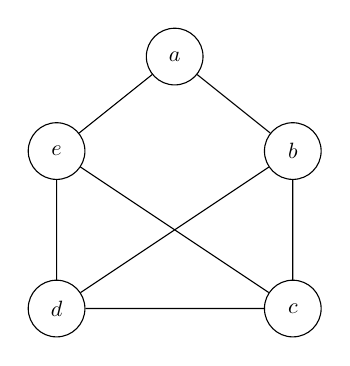
\begin{tikzpicture}[main_node/.style={circle,minimum size = 0.9cm,draw,inner sep=5pt, scale=0.8}]
    \node[main_node] (1) at (0, 4.2) {$a$};
    \node[main_node] (2) at (1.5, 3)  {$b$};
    \node[main_node] (3) at (1.5, 1) {$c$};
    \node[main_node] (4) at (-1.5, 1)  {$d$};
    \node[main_node] (5) at (-1.5, 3) {$e$};
    \draw (1) -- (2) -- (3) -- (4) -- (5) -- (1);
    \draw (2) -- (4);
    \draw (3) -- (5);
\end{tikzpicture}
\hspace{15pt}
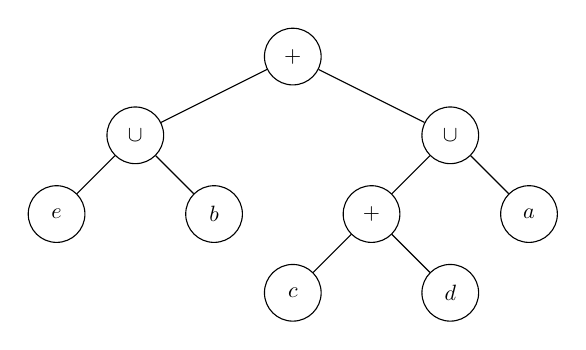
\begin{tikzpicture}[main_node/.style={circle,draw,inner sep=3pt,minimum size = 0.9cm, scale=0.8}]

	\node[main_node] (1) at (2, 0) {$d$};
    \node[main_node] (2) at (0, 0) {$c$};
    \node[main_node] (3) at (3, 1)  {$a$};
    \node[main_node] (4) at (-1, 1) {$b$};
    \node[main_node] (5) at (-3, 1)  {$e$};
    \node[main_node] (6) at (1, 1) {$+$};
    \node[main_node] (7) at (2, 2) {$\cup$};
    \node[main_node] (8) at (-2, 2)  {$\cup$};
   
    \node[main_node] (9) at (0, 3)  {$+$};
 
   
    \draw (9) -- (7) -- (6) -- (1);
    \draw (6) -- (2);
    \draw (7) -- (3);
    \draw (9) -- (8) -- (4);
    \draw (8) -- (5);
 
\end{tikzpicture}
\caption{Graf $G$ in njegovo kodrevo iz primera~\ref{primerGeneriranje}.}
\label{fig:primerGeneriranjaFormule}
\end{figure}

Naj bo  $A = \{e, d\}$. Na sliki hitro opazimo, da množica $A$ ni maksimalna klika, saj ji lahko dodamo še vozlišče $d$, s tem pa povečamo kardinalnost množice. Preverimo to dejstvo z uporabo formule za generiranje maksimalne klike grafa $G$. Najprej zamenjamo se terme v formuli z ustreznimi vrednostmi 0 ali 1 in dobimo formulo
$$(1 \oplus 0) \land ((0 \land 1) \oplus 0),$$ ki jo poenostavimo v $$1 \land (0 \oplus 0),$$ kar je nadalje enako 0. To pomeni, da množica $A$ ni maksimalna klika v grafu $G$.

Oglejmo si sedaj še, kako generiramo maksimalno kliko, ki vsebuje vozlišče $a$. V formulo vnesemo $a=1$ in dobimo $$(e \oplus b) \land ((c \land d) \oplus 1),$$ kar poenostavimo v $$(e \oplus b) \land 1,$$ iz česar sledi $$e \oplus b.$$
To pomeni, da maksimalna klika, ki vsebuje vozlišče $a$, vsebuje tudi ali vozlišče $e$ ali $b$.
\end{primer}
\end{enumerate}

Na povsem enak način lahko obravnavamo tudi iskanje dominantnega števila $\gamma(G)$ ter njegove izpeljanke, varnostnodominantnega števila $\gamma_s(G)$. Ker operacije na notranjih vozliščih zahtevajo precej bolj kompleksen razmislek kot v algoritmih zgoraj, bomo temu posvetili naslednja tri poglavja.

%%%%%%%%%%%%%%%%%%%%%%%%%%%%%%%%%%%%%%%%%%%%%%%%%%%%%%%%%%%%%%%%%
%%%%%%%%%%%%%%%%%%%%%%%%%%%%%%%%%%%%%%%%%%%%%%%%%%%%%%%%%%%%%%%%%
%%%                 VARNOSTNA DOMINACIJA                      %%%
%%%%%%%%%%%%%%%%%%%%%%%%%%%%%%%%%%%%%%%%%%%%%%%%%%%%%%%%%%%%%%%%%
%%%%%%%%%%%%%%%%%%%%%%%%%%%%%%%%%%%%%%%%%%%%%%%%%%%%%%%%%%%%%%%%%

\section{Varnostnodominantno število}\label{sec:varnostnadominacija}
V tem poglavju bomo definirali varnostno dominacijo na grafih in dokazali nekaj izrekov, ki opisujejo varnostnodominantne množice. Prvi izrek karakterizira varnostnodominantno množico z $S$-zunanjo soseščino vozlišča, kot je bila predstavljena leta 2005 v članku \cite{cockayne2005protection}. Rezultat bomo za lažje sklicevanje nekoliko posplošili, nato pa si bomo ogledali še dva pomembna rezultata varnostne dominacije na spojih grafov, ki sta eden izmed temeljev algoritma, ki ga bomo obravnavali v poglavju~\ref{sec:prvialgoritem}.

\medskip
Spomnimo, da je dominantna množica $D$ grafa $G$ taka množica vozlišč, da vsako vozlišče iz $V(G) \setminus D$ leži v soseščini nekega elementa množice $D$. Izpeljanka dominantne množice je varnostnodominantna množica, ki je sama zase tudi dominantna (slika~\ref{dominacija}), le, da velja še dodaten pogoj:
\begin{definicija}
\emph{Varnostnodominantna množica} \index{varnostnodominantna množica} (ang. \emph{security domination set}) $S$ grafa $G$ je taka dominantna množica vozlišč $S \subseteq V(G)$, da je tudi $(S \setminus \{u\}) \cup \{v\}$ dominantna množica. \emph{Varnostnodominantno število $\gamma_s(G)$} \index{varnostnodominantno število} je kardinalnost najmanjše varnostnodominantne množice za graf $G$. Varnostnodominantni množici, katere kardinalnost je enaka varnostnodominantnemu številu, pravimo $\gamma_s$-množica. Rečemo, da $u \in S$ \emph{varuje}\index{varovanje vozlišča} vozlišče $v$, če sta $u$ in $v$ sosedni in velja, da je $(S \setminus \{u\}) \cup \{v\}$ dominantna množica.
\end{definicija}

\begin{figure}[h]
\centering
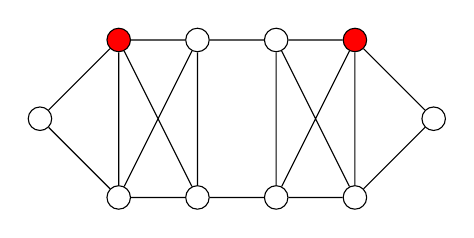
\begin{tikzpicture}[main_node/.style={circle,draw,inner sep=3pt]}]

    \node[main_node] (1) at (1, 1) {};
    \node[main_node, fill=red] (2) at (2, 1)  {};
    \node[main_node] (3) at (3, 0) {};
    \node[main_node] (4) at (2, -1)  {};
    \node[main_node] (5) at (1, -1) {};
    \node[main_node] (6) at (0, -1) {};
    \node[main_node] (7) at (-1, -1)  {};
    \node[main_node] (8) at (-2, 0) {};
    \node[main_node, fill=red] (9) at (-1, 1)  {};
    \node[main_node] (10) at (0, 1) {};
    \draw (1) -- (2) -- (3) -- (4) -- (5) -- (6) -- (7) -- (8) -- (9) -- (10) -- (1);
    \draw (1) -- (4) -- (2) -- (5) -- (1);
    \draw (10) -- (7) -- (9) -- (6) -- (10);
\end{tikzpicture}
\hspace{20pt}
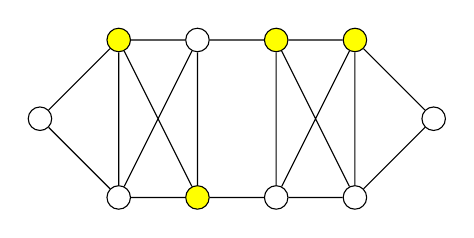
\begin{tikzpicture}[main_node/.style={circle,draw,inner sep=3pt]}]

    \node[main_node, fill=yellow] (1) at (1, 1) {};
    \node[main_node, fill=yellow] (2) at (2, 1)  {};
    \node[main_node] (3) at (3, 0) {};
    \node[main_node] (4) at (2, -1)  {};
    \node[main_node] (5) at (1, -1) {};
    \node[main_node, fill=yellow] (6) at (0, -1) {};
    \node[main_node] (7) at (-1, -1)  {};
    \node[main_node] (8) at (-2, 0) {};
    \node[main_node, fill=yellow] (9) at (-1, 1)  {};
    \node[main_node] (10) at (0, 1) {};
    \draw (1) -- (2) -- (3) -- (4) -- (5) -- (6) -- (7) -- (8) -- (9) -- (10) -- (1);
    \draw (1) -- (4) -- (2) -- (5) -- (1);
    \draw (10) -- (7) -- (9) -- (6) -- (10);
\end{tikzpicture}
\caption{Dominantna množica (na levi) in varnostnodominantna množica (na desni).}  \label{dominacija}
\end{figure}

Koncept varnostne dominacije je v resnici precej naravna posplošitev običajne dominacije, zato navedimo primer, ki ga naravno opiše (povzeto po \cite{pavlic2010rimsko}). Naj bo naš graf omrežje krajev, ki so med seboj (v grafu) sosedni, če med njimi obstaja pot, ki jo je mogoče prevoziti v določenem času. Po državi je potrebno postaviti reševalne postaje tako, da imajo vsi kraji zagotovljeno medicinsko pomoč v določenem času, hkrati pa je reševalnih postaj čim manj. Slednji problem opisuje iskanje dominantne množice v grafu.

Recimo sedaj, da se v nekem kraju zgodi nesreča, zato gre reševalno vozilo na intervencijo. Kraj z reševalno postajo in vsi okoliški kraji, ki jim ta postaja nudi reševalno oskrbo, lahko ostanejo brez nujne medicinske pomoči, vendar pa je reševalno vozilo na voljo v kraju, kamor se je peljal. Želimo zagotoviti, da ima tudi v tem trenutku vsak kraj zagotovljeno medicinsko oskrbo. Iskano minimalno število tako postavljenih reševalnih postaj opisuje varnostnodominantno število.

\subsection{Lastnosti varnostnodominantnih množic}
Najprej navedimo par oznak, ki jih bomo potrebovali. Z oznako $q(G)$ bomo označevali kardinalnost najmanjše množice $U$, tako da je $G \setminus N[U]$ poln graf. Za varnostnodominantno množico $S$ in graf $G$ definiramo vozlišča $u \in V(G) \setminus S$ kot $S$-zunanje sosede vozlišča $v \in S$ \index{$S$-zunanje sosede vozlišča} (ang. $S$-external private neighbour, oznaka $S$-epn), če velja $N(u) \cap S = \{v\}$. Množico vseh $S$-zunanjih vozlišč vozlišča $v$ označimo s \emph{$epn(v, S)$} in jo lahko razumemo kot množico vozlišč, ki je z množico $S$ dominirana le preko vozlišča $v$.

\begin{lema}\label{lemaEPN}
Naj bo $D$ dominantna množica povezanega grafa $G$ in naj bosta $u$ in $v$ poljubni  sosedni si vozlišči iz $V(G)$, da velja $v \in D$ in $u \in V(G) \setminus D$. Tedaj vozlišče $v$ varuje $u$ natanko tedaj, ko velja $epn(v, D)$ $\subseteq N_G[u]$. 
\end{lema}

\begin{proof}
Vozlišča, ki jih dominira le vozlišče $v$---to je $epn(v, D)$, z množico $(D \setminus \{v\}) \cup \{u\}$ niso več dominirana, razen v primeru, ko so sosedna vozlišču $u$. Vsebovanost $epn(v, D) \subseteq N_G[u]$ direktno sledi.
\end{proof}

\begin{izrek}\label{theorem3.1}{\rm{\cite[Proposition 2]{cockayne2005protection}}},{\rm{\cite[Theorem 2.2]{castillano2014secure}}}
Naj bo $G$ povezan graf in $S \subseteq V(G)$. Naslednje trditve so ekvivalentne:
\begin{enumerate}[label=(\roman*)]
\item $S$ je varnostnodominantna množica.
\item Za vsak $u \in V(G) \setminus S$ obstaja tak $v \in S \cap N(u)$, da velja $epn(v,S) \subseteq N[u]$.
\item Za vsak $u \in V(G) \setminus S$ obstaja tak $v \in S \cap N(u)$, da je podgraf $G[\{u,v\} \cup epn(v,S)]$ poln graf.
\end{enumerate}
\end{izrek}

\begin{proof}
$(i) \Rightarrow (ii)$ Naj bo $S$ $\gamma_s$-množica. Za vsak $u \in V(G) \setminus S$, zato obstaja vozlišče $v \in S \cap N(u)$, ki ga varuje. Po lemi~\ref{lemaEPN} velja  $epn(v, D) \subseteq N_G[u]$, zato točka $(ii)$ sledi.

\medskip
$(ii) \Rightarrow (iii)$ Naj bo $u \in V(G) \setminus S$. Po predpostavki obstaja tak $v \in S \cap N_G(u)$, ki varuje vozlišče $u$. Naj bo sedaj množica $A=\{u, v\} \cup epn(v, S)$ in $a$ in $b$ poljubni vozlišči iz $A$, $a \neq b$. Pokazati želimo, da sta vozlišči $a$ in $b$ vedno sosedni. 

\medskip
Če velja $a=u$ in $b=v$, po predpostavki velja, da sta vozlišči sosednji, torej $ab \in E(G)$. Če velja $a=u$ in $b \in epn(v, S)$, po predpostavki velja $epn(v, S) \subseteq N_G[u]$, zato velja $ab \in E(G)$. Če velja $a\in epn(v, S)$ in $b=v$, po definiciji $epn(v, S)$ sledi $ab \in E(G)$. Če pa sta $a,b \in epn(v, S)$, po predpostavki obstaja neko vozlišče  $x \in S \cap N(a)$ (oziroma $x \in S \cap N(b)$), da velja $epn(x,S) \subseteq N[a]$ (oziroma $epn(x,S) \subseteq N[b]$). Po definiciji $epn(v,S)$ sledi, da je edino vozlišče v preseku $S \cap N(a)$ oziroma $s \cap N(b)$ vozlišče $v$, zato sledi  $epn(v,S) \subseteq N[a]$ in $epn(v,S) \subseteq N[b]$. Torej je $ab \in E(G)$, torej je $G[A]$ zares poln graf.

\medskip
$(iii) \Rightarrow (i)$ Naj bo $u \in V(G) \setminus S$ poljubno vozlišče. Po točki 3 obstaja $v \in S \cap N_G(u)$, da je $G[\{u,v\} \cup epn(v,S)]$ poln graf. Da pokažemo, da je $S$ $\gamma_s$-množica, mora biti za poljuben $u$ množica $Y = (S \setminus \{v\}) \cup \{u\}$  dominantna množica za graf $G$. To pomeni, da za poljubno vozlišče $q \not\in Y$ pokažemo, da velja $uw \in E(G)$. 

Če velja $w=v$, potem direktno sledi $uw \in E(G)$.  Zato predpostavimo, da velja $w \neq v$. Tedaj velja $w \not\in S$. Če velja $w \in epn(v,S)$, potem velja $uw \in E(G)$. Obratno, če $w\not\in epn(v, S)$, obstaja $z \in S \setminus \{v\} \subseteq Y$, da velja $zw \in E(G)$.
Ker je bil $u$ poljuben, sledi, da je množica $S$ $\gamma_s$-množica.
\end{proof}

Iz zgornjega izreka hitro sledi naslednja posledica:

\begin{posledica}\label{Observation1ii}
Naj bo $S$ varnostnodominantna množica grafa $G$ in naj bo množica $A \subseteq V(G) \setminus S$ taka množica, da velja $|N_G[A] \cap S| = 1$. Tedaj je $G[A]$ poln graf.
\end{posledica}

\begin{proof} Naj bo $S$ varnostnodominantna množica in $u\in A$ poljubno vozlišče. Po izreku~\ref{theorem3.1} $(iii)$ sledi, da obstaja tak $v \in S \cap N(u)$, da je $G[\{u,v\} \cup epn(v,S)]$ poln graf. Zaradi pogoja za množico $A$, da velja $|N_G[A] \cap S| = 1$ sledi, da obstaja natanko eno možno vozlišče $v$ Ker je $v$ edino vozlišče, ki dominira množico $A$, je $epn(v,S)=A$, zato velja, da je $$G[\{u,v\} \cup epn(v,S)] = G[\{u,v\} \cup A] = G[\{v\} \cup A]$$ poln graf. Sledi, da je tudi $G[A]$ poln graf.
\end{proof}

\begin{primer}\label{primerEPN}
Naj bo $G$ graf na sliki \ref{fig:epn}. Tedaj je množica $S = \{e, h\}$ njegova $\gamma_s$-množica. Vozlišče $h$ varuje vozlišče $a, b, c$ in $d$, vozlišče $e$ pa $g$ in $f$. Tedaj je množica $A = \{a, b, c, d\}$ taka množica, da velja $N_G[A] \cap S = \{h\}$. Po posledici~\ref{Observation1ii} je graf $G[A]$ poln graf.

\begin{figure}[h]
\centering
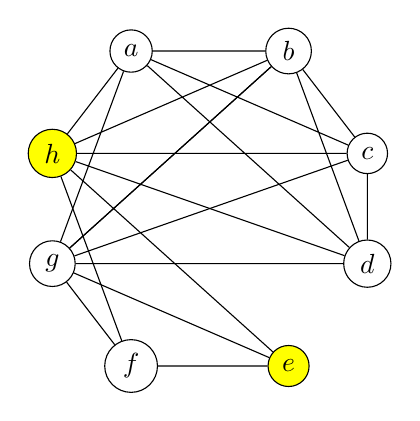
\begin{tikzpicture}[main_node/.style={circle,draw,inner sep=3pt]}]

    \node[main_node] (1) at (1, 2) {$b$};
    \node[main_node] (2) at (2, 0.7)  {$c$};
    \node[main_node] (3) at (2, -0.7) {$d$};
    \node[main_node, fill=yellow] (4) at (1, -2)  {$e$};
    \node[main_node] (5) at (-1, -2) {$f$};
    \node[main_node] (6) at (-2, -0.7) {$g$};
    \node[main_node, fill=yellow] (7) at (-2, 0.7)  {$h$};
    \node[main_node] (8) at (-1, 2) {$a$};
    \draw (7) -- (1) -- (2) -- (3) -- (1) -- (8) -- (2) -- (7) -- (1) -- (6) -- (8) -- (3) -- (7) -- (4) -- (5) -- (6) -- (4);
    \draw (3) -- (6) -- (2) -- (6) -- (1);
    \draw (5) -- (7) -- (8);

\end{tikzpicture}
\caption{Graf $G$ iz primera~\ref{primerEPN}.}  \label{fig:epn}
\end{figure}


\end{primer}

\begin{trditev}\label{theorem3.3}
Naj bo $G$ graf z vsaj enim vozliščem. Potem je $\gamma_s(G) = 1$ natanko tedaj, ko je $G$ poln graf.
\end{trditev}
\begin{proof}
$(\Rightarrow)$ Iz izreka~\ref{theorem3.1} $(iii)$ sledi, da za vsako vozlišče $u \in V(G) \setminus S$ obstaja tako vozlišče $v \in S \cap N(u)$, da je podgraf $G[\{u,v\} \cup epn(v,S)]$ poln. Ker je $S$ tudi dominantna množica, je $epn(v, S) = G$, zato je $G$ poln graf.

\medskip
$(\Leftarrow)$ Graf $G$ je poln graf, ki ga lahko dominira katerokoli vozlišče, zato je varnostnodominantna množica velika vsaj 1.
\end{proof}

V letu 2014 sta Castillano in Ugbinada izdala članek~\cite{castillano2014secure}, v katerem sta preučevala varnostno dominacijo spoja poljubnih grafov in prišla do rezultatov, ki so ključni za algoritem računanja $\gamma_s$ na kografih.

\begin{lema}\label{lemaZaGammaS2}{\rm{\cite[Theorem 2.6 $(i)$]{castillano2014secure}}}
Naj bo $G$ nepoln graf in $x$ in $y$ različni vozlišči, ki dominirata graf $G$. Če velja $$N_G(x) \setminus \{y\} = N_G(y) \setminus \{x\} = V(G) \setminus \{x, y\},$$ je množica $\{x, y\}$ $\gamma_s$-množica in velja $\gamma_s(G) = 2$.
\end{lema}
\begin{proof}
Ker $G$ ni poln graf, po trditvi~\ref{theorem3.3} sledi $\gamma_s(G) > 1$. Naj bo $S = \{x, y\}$ in izberimo poljubno vozlišče $z \in V(G) \setminus S$. Ker je $S$ dominantna množica in sta tako $x$ kot tudi $y$ sosedna vozlišču $z$, je za $z$ vseeno, katero vozlišče iz množice $S$ ga varuje. Recimo, da je to vozlišče $x$. Hitro se prepričamo, da ga $x$ zares varuje, saj je množica $\{y, z\}$ dominantna za $G$---soseščina vozlišča $y$ je po predpostavki enaka $V(G) \setminus \{x, y\}$, vozlišče $x$ pa je sosedno vozlišču $z$. Ker je $z$ izbrano poljubno, je $S$ varnostnodominantna množica.
\end{proof}
Iz te leme tako sledi pomemben rezultat:
\begin{izrek}\label{theorem3.4}
Naj bo $G$ nepoln graf na vsaj dveh vozliščih. Potem velja $\gamma_s(G + K_n) = 2$.
\end{izrek}
\begin{proof} Ker graf $G$ ni poln, tudi $G + K_n$ ni poln. Za $x$ in $y$ izberimo poljubni vozlišči iz množice $V(K_n)$ ter označimo $S = \{x, y\}$. Ker velja $$N_{G+K_n}(x) \setminus \{y\} = N_{G+K_n}(y) \setminus \{x\} = V({G+K_n}) \setminus \{x, y\},$$po lemi~\ref{lemaZaGammaS2} sledi, da je $S$ varnostnodominantna množica in sledi $\gamma_s(G + K_n) = 2$. 
\end{proof}
Drug pomemben izrek opisuje spoj grafa z grafom na enem vozlišču. Sprva si oglejmo lemo, ki nas bo vodila h glavnemu rezultatu.

\begin{lema}\label{lemaSpojZVozliščem}{\rm{\cite[Corollary 2.8]{castillano2014secure}}}
Naj bo $G$ nepoln graf in $K_1$ graf z enim vozliščem $a$. Množica $S \subseteq V( G + K_1)$ je varnostnodominantna množica grafa $G + K_1$ natanko tedaj, ko je izpolnjen eden izmed naslednjih pogojev:
\begin{enumerate}[label=(\roman*)]
\item $S$ je varnostnodominantna množica grafa $G$.
\item $a \in S$ in $N_G[S \setminus \{a\}] = V(G)$.
\item $a \in S$ in $G[V(G) \setminus N_G[S \setminus \{a\}]]$ je poln graf.
\end{enumerate}
\end{lema}
\begin{proof}
$(\Rightarrow)$  Naj bo $S$ varnostnodominantna množica grafa $G + K_1$. Če velja $S \subseteq V(G)$, je $S$ varnostnodominantna tudi za graf $G$. Točka $(i)$ sledi. Privzemimo sedaj $a \in S$. Če je $S \setminus \{a\}$ dominantna množica grafa $G$, sledi točka $(ii)$. Zato privzemimo, da $N_G[S \setminus \{a\}] \neq V(G)$. Vozlišča množice $V(G) \setminus N_G[S \setminus \{a\}]$ so z množico $S$ dominirana le preko vozlišča $a$, torej velja $epn(a, S) = V(G) \setminus N_G[S \setminus \{a\}]$.  Po posledici~\ref{Observation1ii} sledi, da je $G[V(G) \setminus N_G[S \setminus \{a\}]]$ poln graf, kar ustreza $(iii)$.

\medskip
\noindent
$(\Leftarrow)$ Dokaz implikacije razdelimo na tri primere iz izreka:
\begin{enumerate}[label=($\roman*$)]
\item Privzemimo, da je $S$ varnostnodominantna množica grafa $G$. Ker je vozlišče $a$ povezano z vsemi vozlišči iz $V(G)$, je $S$ varnostnodominantna tudi za graf $G + K_1$.
\item Privzemimo $a \in S$ in $N_G[S \setminus \{a\}] = V(G)$. Naj bo $z$ poljubno vozlišče $V(G + K_1) \setminus S = V(G) \setminus (S \setminus \{a\})$ in pokažimo, da je varovano z vozliščem iz $S$. Ker je $S \setminus \{a\}$ dominantna množica za graf $G$, obstaja vozlišče $v \in (S \setminus \{a\})$, ki je sosedno vozlišču $z$. Očitno je množica $(S \setminus \{v\}) \cup \{z\}$ dominantna za $G + K_1$, zato je $S$ varnostnodominantna za $G + K_1$.
\item Privzemimo $a \in S$ in da je $G[V(G) \setminus N_G[S \setminus \{a\}]]$ poln graf. Izberimo poljubno vozlišče $z \in V(G + K_1) \setminus S$. Če je $z \in N_G(S \setminus \{a\})$,  obstaja nek $v\in S \setminus \{a\}$, da sta si $z$ in $v$ sosedna. Množica $(S \setminus \{v\}) \cup \{z\}$ je tedaj tudi dominantna za $G + K_1$, zato je $S$ varnostnodominantna množica za $G + K_1$. Če je $z \in V(G) \setminus N_G[S \setminus \{a\}]$, je množica $(S \setminus \{a\}) \cup \{z\}$ dominantna množica, saj je graf $G[V(G) \setminus N_G[S \setminus \{a\}]]$ poln graf. Množica $S$ je torej varnostnodominantna množica. \qedhere
\end{enumerate}
\end{proof}
Iz leme sledi izrek, ki namiguje na algoritmično uporabo. Pri tem se spomnimo, da z oznako $q(G)$ označujemo kardinalnost najmanjše množice $U$, da je $G \setminus N[U]$ poln graf.
\begin{izrek}\label{theorem3.5}{\rm{\cite[Corollary 2.10]{castillano2014secure}}}
Naj bo $G$ nepoln graf. Potem velja $$\gamma_s(G + K_1) = \min\{\gamma(G) + 1, \gamma_s(G), q(G) + 1\}.$$
\end{izrek}
\begin{proof}
Naj bo $S$ $\gamma_s$-množica grafa $G + K_1$. Privzemimo, da je $S'$ $\gamma_s$-množica grafa $G$ iz točke $(i)$ leme~\ref{lemaSpojZVozliščem}. Tedaj je $S'$ varnostnodominantna množica tudi za graf $G + K_1$, zaradi minimalnosti pa velja $|S| \leq |S'|$, iz česar sledi $\gamma_s(G + K_1) \leq \gamma_s(G)$. 

Če privzamemo lemo~\ref{lemaSpojZVozliščem} $(ii)$, imamo neko dominantno množico $D$, za katero velja $N_G[D] = V(G)$ in $\gamma(G) = |D|$. Če tej množici dodamo vozlišče $\{a\} \in K_1$, po lemi dobimo varnostnodominantno množico $S'$ grafa $G + K_1$. Po minimalnosti velja $|S| \leq |S'|$ in zato tudi $\gamma_s(G + K_1) \leq \gamma(G) + 1$.

Če privzamemo lemo~\ref{lemaSpojZVozliščem} $(iii)$, izberemo najmanjšo tako $U$, da je $G[V(G) \setminus N_G[U]]$ poln graf, kar pomeni, da velja $q(G) = |U|$. Če množici $U$ dodamo še vozlišče $\{a\} \in K_1$, po lemi dobimo varnostnodominantno množico $S'$ grafa $G + K_1$. Po minimalnosti velja $|S| \leq |S'|$ in zato tudi $\gamma_s(G + K_1) \leq q(G) + 1$.

\medskip
Zaradi minimalnosti vse tri primere združimo v $$\gamma_s(G + K_1) = \min\{\gamma(G) + 1, \gamma_s(G), q(G) + 1\}.$$
Izrek sledi.\end{proof}

Spoji grafov so tesno povezani z dvodelnimi grafi, saj so ti njihovi vpeti podgrafi. Če spojimo dve množici vozlišč, $A$ in $B$, ki nimata nobenih povezav, dobimo poln dvodelni graf $K_{m,n}$, kjer je $m$ velikost prve množice $A$ in $n$ velikost druge množice $B$. Očitno je $\gamma(K_{m,n}) = 2$, saj potrebujemo eno vozlišče iz $A$, ki dominira vsa vozlišča iz $B$, ter eno iz množice $B$, ki dominira vsa vozlišča iz $A$.


Če dominantni množici dodamo po eno vozlišče iz množice $A$ in množice $B$, gotovo dobimo varnostnodominantno množico: vozlišči iz $A$ varujeta množico $B$, medtem ko vozlišči iz $B$ varujeta množico $A$. Iz tega sledi
$$\gamma_s(K_{m,n}) \leq 4.$$
Ta rezultat posplošimo za poljuben spoj dveh grafov v naslednji lemi:
\begin{lema} \label{lemma3.6}
Naj bosta $G$ in $H$ grafa z vsaj dvema vozliščema. Za njun spoj velja $$\gamma_s(G + H) \leq 4.$$
\end{lema}
\begin{proof}
Če grafu $G + H$ odstranimo nekaj povezav, dobimo vpet podgraf, ki je poln dvodelni graf $K_{m,n}$ za $m = |G|$ in $n = |H|$. Za $K_{m,n}$ velja ocena $\gamma_s \leq 4$, število $\gamma_S(G + H)$ pa je zaradi več povezav kvečjemu manjše.\end{proof}

\section{Prvi algoritem za izračun $\gamma_s$ na kografih}\label{sec:prvialgoritem}
V tem poglavju si bomo ogledali linearen algoritem za izračun $\gamma_s$ na kografih (v nadaljevanju AY-algoritem), ki sta ga zasnovala T. Araki in R. Yamanaka v članku~\cite{araki2019secure}. Algoritem poleg $\gamma_s(G)$ izračuna tudi $\gamma(G)$ ter $q(G)$. Ker so kografi sestavljeni iz unij in spojev, je za algoritem pomembno kodrevo kografa, kjer je potrebno le določiti, kako se omenjene količine izračunajo na notranjih vozliščih kodrevesa. Dotični algoritem uporablja še bolj specifično binarno kodrevo, kar pomeni, da ima vsako vozlišče bodisi nič, bodisi dva potomca.

V naslednjih podpoglavjih si bomo ogledali izreke, ki izračunajo $\gamma_s$, $\gamma$ in $q$ unije in spoja dveh grafov, nato pa jih združili v omenjeni linearen algoritem.

\subsection{Unija kografov} \label{union}
Najprej si oglejmo, kaj se s števili $\gamma_s(G)$, $\gamma(G)$ in $q(G)$ zgodi pri uniji dveh grafov.

\begin{lema} \label{lemma4.1}
Naj bosta $G$ in $H$ disjunktna kografa. Potem velja:
\begin{enumerate}[label=(\roman*)]
\item $\gamma_s(G \cup H) = \gamma_s(G) + \gamma_s(H)$.
\item $\gamma(G \cup H) = \gamma(G) + \gamma(H)$.
\item $q(G \cup H) = \min\{q(G) + \gamma(H), \gamma(G) + q(H)\}$.
\end{enumerate}
\end{lema}
\begin{proof}
$(i)$ Ker je $G \cup H$ nepovezan graf, potrebujemo na vsaki komponenti svojo varnostnodominantno množico.

\medskip
$(ii)$ Uporabimo enak argument, le da tokrat za dominantno množico.

\medskip
$(iii)$ Pokažimo najprej, da velja $q(G \cup H) \leq \min\{q(G) + \gamma(H), \gamma(G) + q(H)\}$. Naj bo $U \subseteq V(G)$ taka množica, da je $G' = G \setminus N[U]$ poln graf in $|U| = q(G)$. V grafu $H$ poiščimo minimalno dominantno množico $X$, za katero velja $|X| = \gamma(H)$. Če iz grafa $G \cup H$ izbrišemo $N[U \cup X]$, zaradi disjuntknosti grafov $G$ in $H$ dobimo zvezo
$$(G \cup H) \setminus N[U \cup X] = (G \setminus N[U]) \cup (H \setminus N[X]) = G' \cup \emptyset = G'.$$
Ker je $G'$ poln graf, velja $$q(G \cup H) \leq q(G) + \gamma(H).$$ Enako preverimo, da je $q(G \cup H) \leq q(H) + \gamma(G)$. Ker je $q(G \cup H)$ definirana kot minimum kardinalnosti množic s to lastnostjo, sledi $$q(G \cup H) \leq \min\{q(G) + \gamma(H), \gamma(G) + q(H)\}.$$

Pokažimo sedaj, da velja $q(G \cup H) \geq \min\{q(G) + \gamma(H), \gamma(G) + q(H)\}$. Naj bo $U \subseteq V(G \cup H)$ taka množica, da je $(G \cup H) \setminus N[U]$ poln graf in $|U| = q(G \cup H)$. Množico $U$ razdelimo na del $U_G = U \cap V(G)$ in del $U_H = U \cap V(H)$. Da bo $(G \cup H) \setminus N[U]$ res poln graf, mora veljati bodisi $G \setminus N[U_G]$ je prazen in $H \setminus N[U_H]$ je poln graf, bodisi obratno.

Recimo, da velja prva možnost. Potem velja $|U_G| \geq q(G)$ in $|U_H| \geq \gamma(H)$, iz česar sledi $$q(G \cup H) = |U| \geq q(G) + \gamma(H).$$ V drugem primeru ($G \setminus N[U_G]$ je poln in $H \setminus N[U_H]$ je prazen graf) na enak način dobimo oceno
\begin{equation}
q(G \cup H) \geq q(H) + \gamma(G).
\end{equation}
Če obe oceni združimo, dobimo $$q(G \cup H) \geq \min\{q(G) + \gamma(H), \gamma(G) + q(H)\},$$
s tem pa je lema dokazana. \end{proof}

Prvi dve točki izreka lahko direktno posplošimo na unijo več kot dveh grafov. 
\begin{posledica}\label{vecUnij} Če je $G$ končna unija disjunktnih grafov $G_1,..., G_n$, potem velja:
\begin{enumerate}[label=(\roman*)]
\item $\gamma_s(G) = \sum\limits_{i=1}^{l} \gamma_s(G_i).$
\item $\gamma(G) = \sum\limits_{i=1}^{l} \gamma(G_i).$
\end{enumerate}
\end{posledica}

\subsection{Spoj kografov} \label{join}
Druga operacija, ki jo bomo potrebovali pri obravnavi varnostne dominacije na kodrevesu, je spoj grafov. Obravnavajmo najprej nekaj posebnih spojev grafa $G$ in grafa $H$:
\begin{itemize}
\item \textit{eden od grafov $G$ in $H$ je graf na enem vozlišču:} $\gamma_s$ izračunamo z enakostjo iz izreka~\ref{theorem3.5}.
\item \textit{oba grafa sta polna grafa z vsaj dvema vozliščema:} Velja, da je $\gamma_s(G + H) = 1$ natanko tedaj, ko sta $G$ in $H$ polna grafa. To hitro sledi iz izreka~\ref{theorem3.5}.
\item \textit{eden od grafov $G$ in $H$ je polni graf z vsaj dvema vozliščema:} Recimo, da je $G$ poln graf, $H$ pa ne. Po izreku~\ref{theorem3.4} vemo, da je tedaj $\gamma_s(G + H) = 2$.
\end{itemize}

Za grafe z vsaj dvema vozliščema smo v lemi~\ref{lemma3.6} pokazali, da je $\gamma_s(G + H) \leq 4$. Primer, ko je $\gamma_s$ enak 1, smo zgoraj že obravnavali, zato z naslednjimi izreki pokažimo, v katerih primerih je $\gamma_s$ enak številu 2 ali 3. V preostalih primerih bo torej veljalo, da je $\gamma_s = 4$.

\begin{izrek} \label{gamma=2}
Naj bosta $G$ in $H$ nepolna grafa na vsaj dveh vozliščih. Tedaj velja, da je $\gamma_s(G + H) = 2$ natanko tedaj, ko velja ena izmed naslednjih trditev:
\begin{enumerate}[label=(\roman*)]
\item $\gamma_s(G) = 2$ ali $\gamma_s(H) = 2$,
\item $\gamma(G) = 1$ in $\gamma(H) = 1$,
\item $\gamma(G) = 1$ in $q(H) = 1$, ali $q(G) = 1$ in $\gamma(H) = 1$,
\item $q(G) = 1$ in $q(H) = 1$.
\end{enumerate}
\end{izrek}
\begin{proof}
$(\Rightarrow)$ Naj bo $\gamma_s(G + H) = 2$ in $S = \{x,y\}$ varnostnodominantna množica grafa $G + H$. Obravnavajmo dva možna primera glede na to, kje se ti dve vozlišči nahajata.

Recimo, da je $S$ v celoti vsebovan v grafu $G$. Ker $G$ ni poln, velja $\gamma_s(G) \geq 2$. Ker je $\gamma_s(G + H) = 2$, sledi, da je varnostnodominantna množica na manjšem grafu kvečjemu manjša, zato velja $\gamma_s(G + H) = 2$. Enako velja, če je $S$ v celoti vsebovana v grafu $H$. Točka $(i)$ sledi.

Recimo, da je $x \in V(G)$ in $q \in V(G)$. Razdelimo $G$ in $H$ glede na soseščini $N[x]$ in $N[y]$, da velja $V(G) = V_1 \cup V_2$, kjer je $V_1 = N[x]$ in $V_2= V(G) \setminus V_1$, ter $V(H) = U_1 \cup U_2$, kjer je $U_1 = N[y]$ in $U_2= V(H) \setminus U_1$. V primeru, da sta $V_2$ in $U_2$ prazni množici, sledi, da $x$ dominira ves $G$ in $y$ dominira ves $H$, torej velja $\gamma(G) = 1$ in $\gamma(H) = 1$. Točka $(ii)$ sledi.

Drug primer za množici $V_2$ in $U_2$ je, da je ena od njiju prazna, druga pa neprazna. Vzemimo $V_2 = \emptyset$ in $U_2 \neq \emptyset$. Iz $V_2 = \emptyset$ direktno sledi $\gamma(G) = 1$, vozlišča iz $U_2$ pa so dominirana le z vozliščem $x$, torej $U_2 = epn(x, S)$ v grafu $G + H$. Po izreku~\ref{theorem3.1} sledi, da je $H[U_2]$ poln podgraf grafa $H$. Če torej odstranimo soseščino $N[y]$, dobimo poln graf, zato velja $q(H) = 1$. Z enakim razmislekom v primeru $U_2 = \emptyset$ in $V_2 \neq \emptyset$ dobimo rezultat $\gamma(H) = 1$ in $q(G) = 1$, torej točka $(iii)$ sledi.

Ostane še primer, ko sta $V_2$ in $U_2$ obe neprazni množici. Tudi tu opazimo, da po~\ref{theorem3.1} sledi, da sta $G[U_2]$ in $H[V_2]$ polna podgrafa $G$ oziroma $H$, iz česar sledita enakosti $q(G) = 1$ in $q(H) = 1$, kar je natanko točka $(iv)$.

\medskip
$(\Leftarrow)$ Privzemimo, da posamezna trditev velja, in izpeljimo enakost $\gamma_s(G + H) = 2$. Ker grafa $G$ in $H$ nista polna, vemo, da velja $\gamma_s(G + H) \geq 2$.
\begin{enumerate}[label=($\roman*)$]
\item Recimo, da je $\gamma_s(G) = 2$ in $S = \{x,y\}$ varnostnodominantna množica v $G$. $S$ je očitno njena varnostnodominantna množica tudi v $G + H$, zato velja $\gamma_s(G + H) \leq 2$, iz česar sledi enakost $\gamma_s(G + H) = 2$. Enako sklepamo tudi v primeru $\gamma_s(H) = 2$.
\item Privzemimo, da velja $\gamma(G) = 1$ in $\gamma(H) = 1$, $\{x\}$ in $\{y\}$ pa sta dominantni množici za $G$ oziroma za $H$. Ker je v grafu $G + H$ vsako vozlišče iz $G$ povezano z vsakim iz $H$, ja ta množica tudi varnostnodominantna za $G + H$. Sledi $\gamma_s(H) = 2$.
\item Privzemimo, da velja $\gamma(G) = 1$ in $q(H) = 1$. Tedaj obstaja vozlišče $x$, ki dominira ves $G$, ter tako vozlišče $y$, da je podgraf $H \setminus N[y]$ poln. Množica $\{x,y\}$ je tedaj varnostno dominantna množica, saj $x$ varuje $G \cup (H \setminus N[y])$, $y$ pa varuje $N[y] \cup G$. Enako pokažemo za $\gamma(H) = 1$ in $q(G) = 1$.
\item Privzemimo $q(G) = 1$ in $q(H) = 1$. Torej obstajata vozlišči $x \in G$ in $y \in H$, da sta $G \setminus N[x]$ in $H \setminus N[y]$ polna podgrafa. Množica $\{x,y\}$ je tedaj tudi varnostno dominantna množica, saj $x$ varuje del grafa $G \cup (V(H) \setminus N[y])$, vozlišče $y$ pa varuje $H \cup (G \setminus N[x])$. Sledi $\gamma_s(G + H) = 2$.\qedhere
\end{enumerate}
\end{proof}

\begin{izrek} \label{gamma=3}
Naj bosta $G$ in $H$ nepolna grafa na vsaj dveh vozliščih. Tedaj velja, da je $\gamma_s(G + H) = 3$ natanko tedaj, ko velja $\gamma_s(G + H) \neq 2$ in ko velja ena izmed naslednjih trditev:
\begin{enumerate}[label=(\roman*)]
\item $\gamma_s(G) = 3$ ali $\gamma_s(H) = 3$,
\item $\gamma(G) = 2$ ali $\gamma(H) = 2$,
\item $q(G) = 2$ ali $q(H) = 2$.
\end{enumerate}
\end{izrek}
\begin{proof}
$(\Rightarrow)$ Naj bo $\gamma_s(G + H) = 3$ in $S = \{x,y,z\}$ varnostnodominantna množica grafa $G + H$. Obravnavajmo dva možna primera razporeditve vozlišč v $\gamma_s$-množici:
\begin{itemize}
\item Naj bo $\gamma_s$-množica v celoti vsebovana bodisi v $G$, bodisi v $H$, to je $S \subseteq V(G)$ ali $S \subseteq V(H)$. Brez škode za splošnost predpostavimo $S \subseteq V(G)$. $S$ je tedaj varnostnodominantna množica tudi za graf $G$. Ker $G$ ni poln graf, iz izrekov~\ref{theorem3.4} in~\ref{theorem3.5} sledi, da $\gamma_s$-množica ne more biti velikost 1 ali 2, torej velja $\gamma_s(G) \geq 3$. Množica $S$ je torej minimalna varnostnodominantna množica, zato velja $\gamma_s(G)=3$. Enak razmislek velja v primeru $S \subseteq V(H)$, kjer dobimo pogoj $\gamma_s(H)=3$. Točka $(i)$ sledi.
\item Naj bo množica $S$ vsebovana tako v $G$ kot v $H$. Brez škode za splošnost privzemimo $|S \cap V(G)| = 2$ in $|S \cap V(H)| = 1$. Recimo, da $x, y \in V(G)$ in $z \in V(H)$. Razdelimo graf $G$ na $G = V_1 \cup V_2$, kjer je $V_1 = N_G[\{x,y\}]$ in $V_2 = G \setminus V_1$. Podobno graf $H$ razdelimo na $H = U_1 \cup U_2$, kjer je $U_1 = N_H[z]$ in $U_2 = H \setminus U_1$.

Če velja $V_2 = \emptyset$, je množica $\{x,y\}$ dominantna množica za $G$. Ker $G$ ni poln graf, velja $\gamma(G)=2$, iz česar sledi točka $(ii)$.

Če $V_2 \neq \emptyset$, so vozlišča množice $V_2$ v grafu $G + H$ dominirana le z vozliščem $z$. Iz izreka~\ref{theorem3.4} sledi, da je $V_2$ induciran poln graf grafa $G$, kar pomeni, da je $q(G) \leq 2$. S protislovjem pokažimo, da je $q(G)=2$. Recimo, da ni, torej velja $q(G) = 1$. Če je $U_2=\emptyset$, potem velja $\gamma(H)=1$ in po izreku~\ref{gamma=2} sledi $\gamma_s(G+H)=2$, kar vodi do protislovja. Druga možnost je, da velja $U_2 \neq \emptyset$. Ker velja $q(G) = 1$, obstaja tak $v \in (G)$, da je $G \setminus N[v]$ poln graf. Ker je $\{v, z\}$ dominantna množica, kjer vozlišče $v$ varuje podgraf $N[v]$, vozlišče $z$ pa varuje $H \cup G \setminus N[v]$, je tudi varnostnodominantna množica velikosti 2, kar je v protislovju s predpostavko $\gamma_s(G + H) = 3$.

Z dobljenim protislovjem smo ovrgli možnost, da velja $q(G) =1$, zato je $q(G)=2$ in točka $(iii)$ sledi.
\end{itemize}

\noindent $(\Leftarrow)$ Privzemimo $\gamma_s(G+H) \neq 2$ in obravnavajmo varnostnodominantno število grafa $G+H$ glede na naštete trditve iz izreka.
\begin{enumerate}[label=($\roman*)$]
\item Privzemimo, da velja $\gamma_s(G)=3$ ali $\gamma_s(H)=3$. Brez škode za splošnost recimo, da velja $\gamma_(G)=3$, kjer je $S =\{x,y,z\}$ $\gamma_s$-množica za graf $G$. Očitno je $S$ $\gamma_s$-množica tudi za $G+H$, saj so tudi vsa vozlišča v grafu $H$ lahko dominirana kot tudi varovana z množico $S$. Izrek sledi.
\item Privzemimo, da velja $\gamma(G) = 2$ ali $\gamma(H) = 2$. Brez škode za splošnost recimo, da velja $\gamma(G) = 2$, kjer je $S = \{x,y\}$ dominantna množica. Izberimo poljubno vozlišče $z \in H$. Množica $S' = \{x,z,y\}$ je varnostnodominantna množica, saj $x$ in $y$ varujeta podgraf $G$, $z$ pa varuje $H$. Zaradi privzetka $\gamma_s(G+H) \neq 2$ je $S'$ tudi $\gamma_s$-množica. Izrek sledi.
\item Privzemimo, da velja $q(G)=2$ ali $q(H)=2$. Brez škode za splošnost recimo, da velja $q(G)=2$, zato obstaja takšna množica $S =\{x,y\}$, $x,y \in G$, da je $G \setminus N_G[S]$ poln graf. Tedaj izberimo poljubno vozlišče $z \in H$. Množica $S' = \{x,y,z\}$ je varnostnodominantna množica, saj $x$ in $y$ varujeta $N_G[S]$, $z$ pa varuje $H$ in $G \setminus N_G[S]$. Zaradi privzetka $\gamma_s(G+H) \neq 2$ je $S'$ tudi $\gamma_s$-množica. Izrek sledi.\qedhere
\end{enumerate}
\end{proof}

Z zgornjimi izreki smo pokazali, da je varnostnodominantno število za spoj grafov $G$ in $H$ moč izračunati, če poznamo vrednosti $\gamma_s$, $\gamma$ in $q$ grafov $G$ in $H$. Pokažimo še, kako za spoj izračunamo dominantno število ter vrednost $q(G + H)$.

\begin{izrek} \label{theorem4.6}
Naj bosta $G$ in $H$ kografa.
\begin{enumerate}[label=(\roman*)]
\item Če velja $\gamma(G) = 1$ ali $\gamma(H) = 1$, potem velja tudi $\gamma(G + H) = 1$. Sicer velja $\gamma(G + H) = 2$.
\item Če velja $q(G) = 0$ ali $q(H) = 0$, potem velja $q(G + H) = \max\{q(G), q(H)\}$. Sicer velja $q(G + H) = \min\{q(G), q(H)\}$.
\end{enumerate}
\end{izrek}
\begin{proof}
\begin{enumerate}[label=($\roman*)$]
\item Recimo, da velja $\gamma(G) = 1$. To pomeni, obstaja vozlišče $x \in V(G)$, ki je soseden vsem vozliščem $G$. V spoju $G + H$ je vozlišče $x$ tako sosedne vsem vozliščem grafa $G$ in grafa $H$, kar pomeni, da je $\gamma(G + H) = 1$. Enako razmislimo tudi v primeru $\gamma(H) = 1$.

Če noben od dveh pogojev ne velja, potrebujemo eno (poljubno) vozlišče iz $H$, ki bo dominiralo $G$, in eno (poljubno) vozlišče $H$, ki bo dominiralo $G$. Iz tega sledi $\gamma(G + H) = 2$.
\item Če je kateri od grafov $G$ ali $H$ poln (torej velja $q(G) = 0$ ali $q(H) = 0$), poln graf v $G + H$ dobimo tako, da grafu $G + H$ odstranimo zaprto soseščino nekaterih vozlišč. Če je na primer $G$ poln graf, $H$ pa ne, je število teh vozlišč natanko $q(H)$. Če je $H$ poln graf, $G$ pa ne, je število $q(G + H)$ enako $q(G)$. Če sta $G$ in $H$ polna, je $G + H$ poln graf, zato velja $q(G + H) = 0$ . Če vse te rezultate združimo, dobimo enakost $q(G + H) = \max\{q(G), q(H)\}$.

Če noben od dveh grafov ni poln, potem odstranimo soseščine vozlišča le tistemu grafu, ki ima manjše $q$ število. Recimo, da je to $G$. Po odstranjevanju vozlišč smo zato odstranili tudi vsa vozlišča grafa $H$, saj v $G + H$ graf $H$ leži v soseščini vsakega vozlišča grafa $G$, torej smo dobili poln graf, ki je podgraf grafa $G$. Podoben premislek sledi za primer, ko velja $q(H) < q(G)$. Rezultata združimo v enakost $q(G + H) = \min\{q(G), q(H)\}$.
\end{enumerate}
\end{proof}

\subsection{Algoritem AY}

\begin{algorithm}[h]
\caption{Algoritem AY: Varnostna dominacija na kografih}\label{alg:araki}
\begin{algorithmic}[1]
\Function{izračunajGamaS}{Cotree $T_G$, Node $t_i$}
  \If {$t_i$ je list} \textbf{return} (1, 1, 0, 1); \EndIf
  \State $t_l$ $\leftarrow$ levi potomec od $t_i$;
  \State $t_r$ $\leftarrow$ desni potomec od $t_i$;
  \State $(s_l, g_l, q_l, n_l) \leftarrow$ izračunajGamaS($T_G$, $t_l$);
  \State $(s_r, g_r, q_r, n_r) \leftarrow$ izračunajGamaS($T_G$, $t_r$);
  \If {$t_i$ je unija}
  \State \textbf{return} ($s_l + s_r, g_l + g_r, \min\{q_l, g_r, g_l, q_r), n_l + n_r\}$;
  \Else
  	\If {$s_l = 1$ in $s_r = 1$} $\gamma_s \leftarrow 1$;
  	\ElsIf {$s_l = 1$ in $s_r \geq 2$}
    	\If {$n_l = 1$} $\gamma_s \leftarrow \min\{g_r + 1, s_r, q_r + 1\}$ \Else \State $\gamma_s \leftarrow 2$; \EndIf
  	\ElsIf {$s_r = 1$ in $s_l \geq 2$}
  		\If {$n_l = 1$} $\gamma_s \leftarrow \min\{g_l + 1, s_l, q_l + 1\}$ \Else   \State$\gamma_s \leftarrow 2$; \EndIf
  	\Else
    	\If {eden od pogojev iz~\ref{gamma=2} drži} $\gamma_s \leftarrow 2$;
  		\ElsIf {eden od pogojev iz~\ref{gamma=3} drži} $\gamma_s \leftarrow 3$;
  		\Else
  		    \State $\gamma_s \leftarrow 4$; \EndIf
  	\EndIf
  \EndIf
  
  \If {$g_l = 1$ ali $g_r = 1$} $\gamma \leftarrow 1$
  \Else
    \State $\gamma \leftarrow 2$;
  \EndIf
  
  \If {$q_l = 0$ ali $q_r = 0$} $q \leftarrow \max\{q_l, q_r\}$
  \Else
    \State $q \leftarrow \min\{q_l, q_r\}$;
  \EndIf
  
  \State \textbf{return} ($\gamma_s, \gamma, q, n_l + n_r$);
\EndFunction
\end{algorithmic}
\end{algorithm}
Algoritem~\ref{alg:araki} za računanje $\gamma_s$ sprejme binarno kodrevo, vrne pa varnostnodominantno število, dominantno število, vrednost $q$ ter število vozlišč grafa. Skonstruiran je rekurzivno, kjer za liste določi znane vrednosti teh štirih števil, nato pa glede na notranja vozlišča kodrevesa računa vrednosti navzgor po drevesu. Ker je kodrevo binarno, ima vsako notranje vozlišče natanko dva potomca, kar pomeni, da vrednosti $\gamma_s$, $\gamma$ in $q$ na vsakem koraku računamo le na spoju/uniji dveh grafov, kakor smo to obravnavi v zgornjih izrekih.

\begin{izrek}
Algoritem AY pravilno izračuna varnostnodominantno število za poljuben kograf $G$ v času $O(m(G) + n(G))$.
\end{izrek}
\begin{proof}
Za podan graf $G$ poiščemo ustrezno binarno kodevo $T_G$, kar lahko napravimo v $O(n(G) + m(G))$ (z linearnim algoritmom \cite[Algorithm Cograph-recognition]{corneil1985linear} konstruiramo kodrevo, nato pa ga v linearnem času prilagodimo v binarnega, kot je opisano na koncu poglavja \ref{kografiInKodrevesa}). Nato pokličemo algoritem~\ref{alg:araki} z vhodnimi podatki $T_G$ in korenom kodrevesa. Da zares dobimo pravo varnostnodominantno število, nam zagotavljajo izreki v podpoglavjih~\ref{union} in~\ref{join}.

Vsako binarno drevo ima $2n - 1$ vozlišč, kjer je $n$ število listov drevesa. Če ima graf $G$ $n$ vozlišč, to pomeni, da ima kograf $n$ listov in $n-1$ notranjih vozlišč. Algoritem rekurzivno kličemo na potomcih korena drevesa, ki so notranja vozlišča, vozlišč ne ponavljamo. Ko pridobimo vrednosti za $\gamma_s$, $\gamma$, $q$ in $n$ nižje ležečih vozlišč v drevesu, lahko nove štiri vrednosti izračunamo v konstantnem času. Celoten algoritem tako deluje v času $O(n)$, skupaj z izgradnjo kodrevesa pa v $O(n + m)$.
\end{proof}


\begin{figure}[h]
\centering
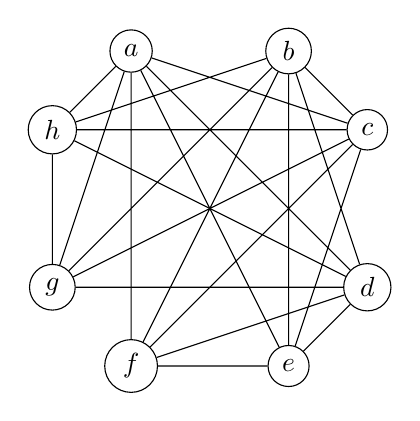
\begin{tikzpicture}[main_node/.style={circle,draw,inner sep=3pt]}]

    \node[main_node] (1) at (1, 2) {$b$};
    \node[main_node] (2) at (2, 1)  {$c$};
    \node[main_node] (3) at (2, -1) {$d$};
    \node[main_node] (4) at (1, -2)  {$e$};
    \node[main_node] (5) at (-1, -2) {$f$};
    \node[main_node] (6) at (-2, -1) {$g$};
    \node[main_node] (7) at (-2, 1)  {$h$};
    \node[main_node] (8) at (-1, 2) {$a$};
    \draw (1) -- (2) -- (4) -- (5) -- (8) -- (7) -- (6) -- (8) -- (4) -- (1) -- (7) -- (2) -- (8) -- (3) -- (1) -- (5) -- (2) -- (6) -- (1);
    \draw (7) -- (3) -- (6);
    \draw (5) -- (3) -- (4);
\end{tikzpicture}
\caption{Kograf $G$, na katerem je bil zagnan algoritem AY.}  \label{fig:skica-araki-graf}
\end{figure}


\begin{figure}[h!]
\centering
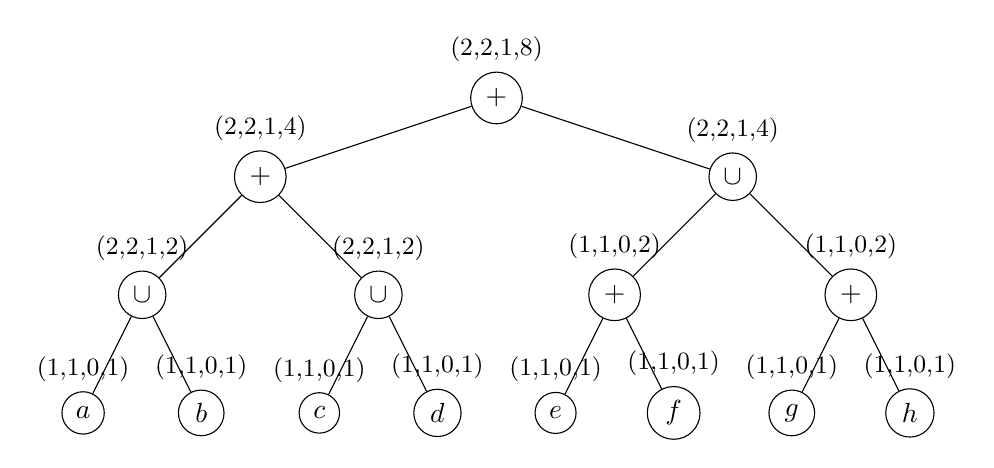
\begin{tikzpicture}[main_node/.style={circle,draw,inner sep=3pt]}]

	\node[main_node, label=\small{(1,1,0,1)}, draw] (1) at (-5.25, -1) {$a$};
    \node[main_node, label=\small{(1,1,0,1)}] (2) at (-3.75, -1) {$b$};
    \node[main_node, label=\small{(1,1,0,1)}] (3) at (-2.25, -1)  {$c$};
    \node[main_node, label=\small{(1,1,0,1)}] (4) at (-0.75, -1) {$d$};
    \node[main_node, label=\small{(1,1,0,1)}] (5) at (0.75, -1)  {$e$};
    \node[main_node, label=\small{(1,1,0,1)}] (6) at (2.25, -1) {$f$};
    \node[main_node, label=\small{(1,1,0,1)}] (7) at (3.75, -1) {$g$};
    \node[main_node, label=\small{(1,1,0,1)}] (8) at (5.25, -1)  {$h$};
    
    \node[main_node, label=\small{(2,2,1,2)}] (9) at (-4.5, 0.5)  {$\cup$};
    \node[main_node, label=\small{(2,2,1,2)}] (10) at (-1.5, 0.5) {$\cup$};
    \node[main_node, label=\small{(1,1,0,2)}] (11) at (1.5, 0.5) {$+$};
    \node[main_node, label=\small{(1,1,0,2)}] (12) at (4.5, 0.5)  {$+$};
    
    \node[main_node, label=\small{(2,2,1,4)}] (13) at (-3, 2) {$+$};
    \node[main_node, label=\small{(2,2,1,4)}] (14) at (3, 2)  {$\cup$};
    
    \node[main_node, label=\small{(2,2,1,8)}] (15) at (0,3)  {$+$};

   
    \draw (15) -- (13) -- (9) -- (1);
    \draw (13) -- (10) -- (3);
    \draw (9) -- (2);
    \draw (10) -- (4);
    
     \draw (15) -- (14) -- (11) -- (5);
    \draw (14) -- (12) -- (7);
    \draw (12) -- (8);
    \draw (11) -- (6);
\end{tikzpicture}
\caption{Kodrevo za graf $G$ s slike~\ref{fig:skica-araki-graf}, na katerem je bil zagnan algoritem AY.}  \label{skica araki}
\end{figure}

\begin{primer}
Primer zagnanega algoritma na grafu $G$ s slike~\ref{fig:skica-araki-graf} lahko ponazorimo na kografu, kot je prikazano na sliki~\ref{skica araki}. Vsakemu vozlišču $c_i$ kografa algoritem priredi vrednosti $\gamma_s(T_G(c_i))$, $\gamma(T_G(c_i))$, $q(T_G(c_i))$ in $n(T_G(c_i))$, kar je na sliki prikazano s pomočjo seznamov dolžine 4. Algoritem poženemo na korenu kodrevesa, posledično pa se rekurzivno pokliče na vseh vozliščih, pri čemer nove vrednosti računa od spodaj navzgor. Na prvem nivoju tako vsem listom priredi vrednosti $(1,1,0,1)$, saj sta $\gamma_s$ in $\gamma$ za list enaka 1, vrednost $q$ je enaka 0, število vozlišč pa je enako 1. Nadaljujemo na drugem nivoju, kjer ločimo primera levo, kjer imamo notranja vozlišča unije, ter primera desno z vozlišči spoja. Vrednosti za unijo izračunamo s pomočjo vrstice 8 v algoritmu~\ref{alg:araki}, vrednosti za spoj z drugega nivoja slike~\ref{skica araki} pa z vrsticami 10, 21, 23 in 25. Na tretjem nivoju je na levi vozlišče spoja, zato uporabimo vrstice 18 (saj velja pogoj leme~\ref{gamma=2} $(i)$), 22, 24 in 25, vrednosti za unijo na desni pa s pomočjo vrstice 8.

Kot zadnje vozlišče obravnavamo koren drevesa. Označen je s $+$, zato za izračun uporabimo vrstice 18, 22, 24 in 25 ter dobimo vrednosti $(2,2,1,8)$.  To pomeni, da je varnostnodominantno število je enako 2 (primer $\gamma_s$-množice pa je množica $\{a, b\}$), dominantno število je enako 2 (primer $\gamma$-množice je prav tako množica $\{a, b\}$), vrednost $q(G)$ je enaka 1 (če odstranimo zaprto soseščino vozlišča $c$, nam ostane vozlišče $d$, ki je poln graf), graf pa ima 8 vozlišč.
\end{primer}

\section{Drugi algoritem za izračun $\gamma_s$ na kografih}\label{sec:drugialgoritem}
V tem poglavju si bomo ogledali še en algoritem za izračun $\gamma_s$ v kografih avtorjev D. Pradhan, A. Jha in S. Banerjee, ki je bil objavljen v članku~\cite{jha2019secure} prav tako leta 2019, a se problema loti na nekoliko drugačen način. Algoritem sprejme kograf $G$, izračuna njegovo kodrevo $T_G$ (ki ni nujno binarno!), nato pa $\gamma_s$ poračunamo rekurzivno - vrednost $\gamma_s$ tako najprej določimo listom (ta vrednost je za liste enaka 1), nato pa nadaljujemo z vozlišči po drevesu navzgor, kjer uporabimo vrednosti, določene na prejšnji iteraciji. Tako ločimo postopek računanja glede na tip vozlišča, v katerem se nahajamo. Če je notranje vozlišče $u$ na trenutni iteraciji označeno z oznako $\cup$, s pomočjo posledice~\ref{vecUnij} seštejemo $\gamma_s(w)$ za vsakega potomca $w$ vozlišča $u$. Nekoliko težje je izračunati $\gamma_s$ za spoj grafov: sprva bomo definirali lastnost $\mathcal{R}$ za vozlišča kodreves ter lastnosti $\mathcal{P}$ in $\mathcal{P^*}$ za kografe, z njihovo pomočjo pa bomo nato obravnavali različne primere in kombinacije potomcev notranjih vozlišč z oznako $+$. Obravnavani primeri nas bodo vodili do končne oblike algoritma in zagotavljali njegovo pravilno delovanje.

V nadaljevanju bomo vedno predpostavili, da je obravnavani graf povezan, sicer lahko število $\gamma_s$ poiščemo na posameznih komponentah ter jih seštejemo. Graf $G$ v naslednjih definicijah in lemah je torej kograf, ki ima za koren pripadajočega kodrevesa $T_G$ vozlišče z oznako $+$.

\subsection{Tehnične priprave za algoritem}
Za omenjeni algoritem bomo vpeljali lastnost $\mathcal{R}$ za vozlišča kodreves ter lastnost $\mathcal{P}$ in $\mathcal{P^*}$ za kografe, ki bodo igrale pomembno vlogo v določanju $\gamma_s$ v kografu. Navedimo sprva definicije vseh treh lastnosti ter njihove karakterizacije, ki jih bo lahko uporabil tudi algoritem.

\begin{definicija} Naj bo $G$ kograf in $T_G$ njegovo pripadajoče kodrevo. Vozlišče $u\in T_G$ ima \emph{lastnost $\mathcal{R}$}, če ima oznako $\cup$, ima natanko dva potomca $x$ in  $y$ ter velja $\gamma(T_G(x)) = \gamma_s(T_G(y)) = 1$.
\end{definicija}

\begin{primer}\label{primerR}
Naj bo $G$ kograf, kot je prikazan na sliki~\ref{fig:primerRgraf} s pripadajočim kodrevesom (na sliki~\ref{fig:primerRdrevo}). Rdeče obarvano vozlišče ima lastnost $R$, saj je podgraf na vozliščih iz množice $\{a, b, d, e, f, g\}$ nepovezan in ima natanko dva potomca. Dominantna množica podgrafa na vozliščih $\{d, e, f, g\}$ (obarvano z rumeno) je singleton $\{f\}$, medtem ko je $\gamma_s$-množica podgrafa na vozliščih $\{a,  b\}$ (obarvano z oranžno) singleton $\{a\}$.
\end{primer}

\begin{figure}[h]
\centering
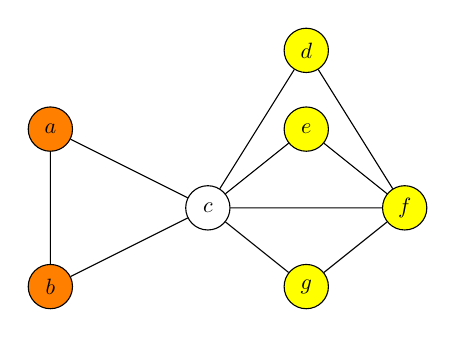
\begin{tikzpicture}[main_node/.style={circle,draw,minimum size=2em,inner sep=1, scale=0.8]}]
    \node[main_node, fill=orange] (1) at (-2, 1) {$a$};
    \node[main_node, fill=orange] (2) at (-2, -1)  {$b$};
    \node[main_node] (3) at (0, 0) {$c$};
    \node[main_node, fill=yellow] (4) at (1.25, 2)  {$d$};
    \node[main_node, fill=yellow] (5) at (1.25,1) {$e$};
    \node[main_node, fill=yellow] (6) at (2.5,0) {$f$};
    \node[main_node, fill=yellow] (7) at (1.25,-1)  {$g$};
    \draw (3) -- (1) -- (2) -- (3) -- (4) -- (6) -- (5) -- (3) --(6) -- (7) -- (3) -- (1);
\end{tikzpicture}
\caption{Graf $G$ iz primera~\ref{primerR}}
\label{fig:primerRgraf}
\end{figure}

\begin{figure}[h]
\centering
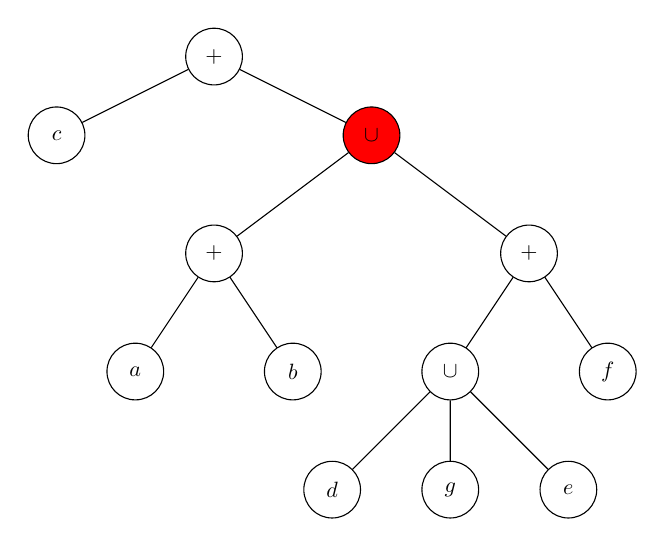
\begin{tikzpicture}[main_node/.style={circle,draw,inner sep=3pt,minimum size = 0.9cm, scale=0.8}]

	\node[main_node] (12) at (-2, 4) {$+$};
    \node[main_node] (10) at (-4, 3) {$c$};
	\node[main_node] (11) at (2.5, -1.5) {$e$};
    \node[main_node] (1) at (1, -1.5) {$g$};
    \node[main_node] (2) at (-0.5, -1.5) {$d$};
    \node[main_node] (3) at (3, 0)  {$f$};
    \node[main_node] (4) at (-1, 0) {$b$};
    \node[main_node] (5) at (-3, 0)  {$a$};
    \node[main_node] (6) at (1, 0) {$\cup$};
    \node[main_node] (7) at (2, 1.5) {$+$};
    \node[main_node] (8) at (-2, 1.5)  {$+$};
   
    \node[main_node, fill=red] (9) at (0, 3)  {$\cup$};
 
   
    \draw (9) -- (7) -- (6) -- (1);
    \draw (6) -- (2);
    \draw (7) -- (3);
    \draw (9) -- (8) -- (4);
    \draw (8) -- (5);
     \draw (11) -- (6);
     \draw (10) -- (12) -- (9);
 
\end{tikzpicture}
\caption{Kodrevo kografa s slike~\ref{fig:primerRgraf}. Rdeče obarvano vozlišče ima lastnost $\mathcal{R}$.}
\label{fig:primerRdrevo}
\end{figure}



\begin{lema}\label{Lema1}
Naj bo $T_G$ kodrevo za kograf $G$ in $u$ neko vozliše v $T_G$. Tedaj ima $u$ lastnost $\mathcal{R}$ natanko tedaj, ko je $T_G(u)$ nepovezan in obstaja vozlišče $w'\in T_G(u)$, da je $V(T_G(u)) \setminus N_{T_G}[w']$ klika.
\end{lema}
\begin{proof}
$(\Rightarrow)$ Naj bo $u$ vozlišče z lastnostjo $\mathcal{R}$ in naj bosta $x$ in $y$ njegova potomca, za katera velja $\gamma(T_G(x)) = \gamma_s(T_G(y)) = 1$. Po opombi~\ref{Observation 5} ima graf $G$ dve komponenti za povezanosti, to sta $T_G(x)$ in $T_G(y)$. Naj bo $\{w\}$ dominantna množica grafa $T_G$, kar pomeni, da je vozlišče $w$ povezano z vsemi vozlišči komponente $T_G(x)$ ter z nobenim vozličem komponente $T_G(y)$. Sledi, da velja $V(T_G(u)) \setminus N_{T_G(u)}[w] = V(T_G(y))$. Ker velja $\gamma_s(T_G(y))=1$, po trditvi~\ref{theorem3.3} sledi, da je $V(T_G(y))$ klika. 

\medskip
$(\Leftarrow)$ Naj bo $T_G(u)$ nepovezan graf in $w$ tako vozlišče, da je $V(T_G(u)) \setminus N_{T_G}[w']$ klika. Radi bi pokazali, da ima vozlišče $u$ lastnost $\mathcal{R}$.
Najprej pokažimo, da je $u$ vozlišče z oznako $\cup$. Ker je $T_G(u)$ nepovezan graf, $u$ ne more biti list, zato je notranje vozlišče. Prav tako zaradi nepovezanosti ne more imeti oznake $+$, zato sledi, da ima oznako $\cup$.

Pokažimo, da ima vozlišče $u$ natanko dva potomca. Naj bodo $T_G(u_1),...,T_G(u_k)$, $k \geq 2$, komponente grafa $T_G(u)$, kjer so $u_i$, $i \in [k]$, potomci vozlišča $u$. Brez škode za splošnost lahko predpostavimo, da se vozlišče $w$ nahaja v komponenti $T_G(u_1)$, zaradi nepovezanosti grafa $T_G(u)$ pa velja, da $w$ ni povezan z nobenim vozliščem iz komponent $T_G(u_i)$ za $i \geq 2$. Recimo sedaj, da je $k > 2$. Potem obstajata $a \in T_G(u_2)$ in $b \in T_G(u_3)$. Ker sta $a$ in $b$ iz dveh različnih komponent, velja $ab \not\in E(T_G)$, ker pa se nahajata v drugi komponenti kot $w$, pa velja $a,b \not\in N_{T_G(u)}[w']$. Sledi, da $V(T_G(u)) \setminus N_{T_G(u)}[w']$ ni klika, kar vodi do protislovja, torej ima graf $T_G(u)$ le dve komponenti za povezanost.

Pokažimo, da velja $\gamma(T_G(u_1)) = \gamma_s(T_G(u_2)) = 1$. Po predpostavki obstaja tako vozlišče $w$, da je $V(T_G(u)) \setminus N_{T_G}[w']$ klika. Recimo sedaj, da enakost $\gamma(T_G(u_1)) = 1$ ne velja, kar pomeni, da obstaja neko vozlišče $y \in T_G(u_1)$, za katerega velja $yw \not\in E(T_G(u))$. Zaradi lastnosti komponent za povezanost prav tako ne obstaja povezava med vozliščem $y$ in katerim koli vozliščem v grafu $T_G(u_2)$, kar je v protislovju s pogojem, da je množica $V(T_G(u)) \setminus N_{T_G(u)}[w]$ klika. Pogoj $\gamma(T_G(u_1)) = 1$ torej sledi. Vozlišče $w$ je zato povezano z vsemi vozlišči komponente za povezanost $T_G(u_1) \setminus \{w\}$, velja pa tudi $V(T_G(u)) \setminus N_{T_G(u)}[w] = V(T_G(u_2))$, iz česar sledi, da je množica $V(T_G(u_2))$ klika. Po trditvi~\ref{theorem3.3} sledi $\gamma_s(T_G(u_2)) = 1$.

S temi tremi točkami smo dokazali, da ima vozlišče $u$ lastnost $\mathcal{R}$.
\end{proof}

Naslednji dve lastnosti se ne nanašata več samo na vozlišče, vendar na celoten kograf, ki je dobljen kot spoj več manjših grafov.

\begin{definicija}Naj bo $G$ kograf, dobljen s spojem kografov $G_1, \dots, G_l$, $ l \geq 2$. Graf $G$ ima \emph{lastnost $\mathcal{P}$}, če obstajata vozlišči $x,y\in V(G)$, da je $\{x, y\}$ dominantna množica in vsaka izmed $V(G) \setminus N_G[x]$ in $V(G) \setminus N_G[y]$ je ali prazna množica ali klika.
\end{definicija}
\begin{definicija}Naj bo $G$ kograf, dobljen s spojem grafov $G_1, \dots, G_l$, $l \geq 2$. Graf $G$ ima \emph{lastnost $\mathcal{P}^*$}, če velja
\begin{enumerate}[label=($\roman*$)]
\item $G$ je poln graf \textbf{ali}
\item $\gamma(G) = 2$ in obstaja tako vozlišče $w \in V(G)$, da je $V(G) \setminus N_G[w]$ klika.
\end{enumerate}
\end{definicija}

\begin{primer}
Kograf s slike~\ref{fig:primerRgraf} ima lastnost $\mathcal{P}$, nima pa lastnosti $\mathcal{P^*}$.
Za lastnost $\mathcal{P}$ vlogo vozlišč $x$ in $y$ prevzameta vozlišči $c$ in $f$. Unija njunih zaprtih soseščin tvori množico $V(G)$, množici vozlišč brez njunih soseščin pa sta $\{f\}$ za vozlišče $c$ in $\{a, b, c\}$ za vozlišče $f$. Ker sta podgrafa na množici vozlišč $V(G) \setminus N_G[c] = \{f\}$  ter $V(G) \setminus N_G[f] = \{a, b, c\}$ polna grafa, je lastnost res izpolnjena.
Lastnosti $\mathcal{P^*}$ kograf nima, saj je množica $\{c\}$ dominantna množica in pogoj $\gamma(G)=2$ ni izpolnjen.
\end{primer}

\begin{primer}\label{primerP}
Naj bo $k \in \mathbb{N}$ in $K_k$ poln graf z vozlišči $\{a_1, \dots, a_k\}$. Družina kografov $G_k$ (na sliki \ref{fig:primerPgraf}) je definirana kot graf z množico vozlišč $V(G_k) = V(K_k) \cup \{b, c, d, e\}$ in množico povezav $$E(G_k) = E(K_k) \cup \{bc, bd, be\} \cup \{ca_i, da_i, ea_i, i \in [k]\}.$$

\begin{figure}[h]
\centering
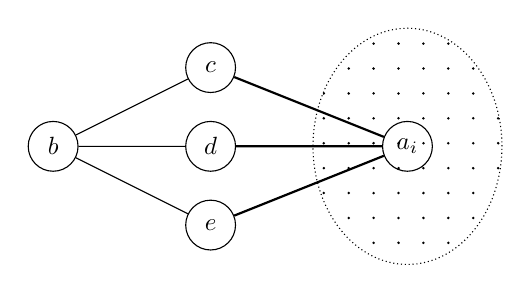
\begin{tikzpicture}[main_node/.style={circle,draw,minimum size=2em,inner sep=1, scale=0.9}]
\usetikzlibrary{shapes}
\pgfdeclarepatternformonly{mynewdots}{\pgfqpoint{-1pt}{-1pt}}{\pgfqpoint{0.5pt}{0.5pt}}{\pgfqpoint{9pt}{9pt}}% original definition: \pgfqpoint{3pt}{3pt}
{%
  \pgfpathcircle{\pgfqpoint{0pt}{0pt}}{.5pt}%
  \pgfusepath{fill}%
}%
\usetikzlibrary{patterns}
    \node[main_node] (1) at (-2,0) {$b$};
    \node[main_node] (2) at (0,1) {$c$};
    \node[main_node] (3) at (0,0) {$d$};
    \node[main_node] (4) at (0,-1) {$e$};
    \node[main_node, font=\bfseries] (5) at (2.5,0) {$a_i$};
    \draw[densely dotted, pattern=mynewdots] (2.5,0) ellipse (1.2 and 1.5);
    
    \draw (2) -- (1) -- (3);
    \draw (4) -- (1);
    \draw[thick] (2) -- (5) -- (3);
    \draw[thick] (5) -- (4);

\end{tikzpicture}
\caption{Družina grafov $G_k$. Območje s pikami predstavlja poln graf $K_k$ na vozliščih $\{a_1, \dots, a_k\}$, odebeljene povezave pa predstavljajo spoj grafa $K_k$ z neodvisno množico $\{c, d, e\}$.}
\label{fig:primerPgraf}
\end{figure}

\begin{figure}[h]
\centering
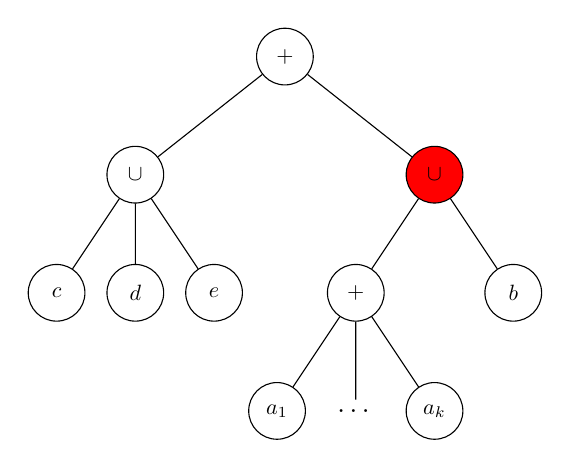
\begin{tikzpicture}[main_node/.style={circle,draw,inner sep=3pt,minimum size = 0.9cm, scale=0.8}]

	\node[main_node] (1)   at (1.1,0.5) {$+$};
    \node[main_node] (2)   at (-0.8, -1) {$\cup$};
	\node[main_node, fill=red] (3)   at (3,-1){$\cup$};
    \node[main_node] (4)   at (-1.8, -2.5){$c$};
    \node[main_node] (5)   at (-0.8,-2.5) {$d$};
    \node[main_node] (6)   at (0.2,-2.5) {$e$};
    \node[main_node] (7)   at (2,-2.5) {$+$};
    \node[main_node] (8)   at (4,-2.5) {$b$};
    \node[main_node] (9)   at (1,-4) {$a_1$};
    \node[] (10)   at (2,-4) {$\dots$};
     \node[main_node] (11)   at (3,-4) {$a_k$};
    
    \draw (4) -- (2) -- (5);
    \draw (6) -- (2) -- (1) -- (3) -- (7) -- (9);
    \draw (8) -- (3);
    \draw (10) -- (7) -- (11);

\end{tikzpicture}
\caption{Kodrevo družine kografov $G_k$ s slike~\ref{fig:primerPgraf}. Rdeče obarvano vozlišče ima lastnost $\mathcal{R}$.}
\label{fig:primerPdrevo}
\end{figure}

Grafi $G_k$ imajo tako lastnost $\mathcal{P}$ kot tudi lastnost $\mathcal{P^*}$. Dominantna množica grafa je na primer $\{a_1, c\}$, kar pomeni, da velja $\gamma(G) \leq 2$. Ker vozlišče $b$ ni povezano z nobenim vozliščem $a_i$ za poljuben $i \in [k]$, velja $\gamma(G) \neq 1$, zato sledi $\gamma(G) = 2$. Če množici vozlišč odstranimo $N_G[c]$, dobimo množico $K_k$, ki je poln graf. Kograf $G$ zato zadošča lastnosti  $\mathcal{P^*}$. 
Graf zadošča tudi lastnosti $\mathcal{P}$, saj sta vozlišči $a_1$ in $c$ taki vozlišči, da je $\{a_1, c\}$ dominantna množica ter da sta $V(G) \setminus N_G[a_1]$  in $V(G) \setminus N_G[c]$ polna grafa.
\end{primer}


Lastnost $\mathcal{R}$ in $\mathcal{P}$ se povežeta z naslednjo lemo.

%%%%%%%%%%%%%%%%%%%%%%%%%%%%%%%%%%%%%%%%%%%%%%%%%%%%%%%%
\begin{lema}\label{Lema2} Naj bo $T_G$ kodrevo za kograf $G$ in $c$ neko notranje vozlišče z oznako $+$. Tedaj ima $T_G(c)$ lastnost $\mathcal{P}$ natanko tedaj, ko je izpolnjen eden od naslednjih pogojev:
\begin{enumerate}[label=($\roman*$)]
\item Obstajata vsaj dva potomca vozlišča $c$, ki sta ali list ali vozlišče z oznako $\mathcal{R}$.
\item Obstajata vsaj dva potomca vozlišča $c$, kjer je en od njiju vozlišče $u$ z oznako $\mathcal{R}$, graf $T_G(u)$ pa je unija dveh polnih grafov.
\end{enumerate}
\end{lema}

\begin{proof}
$(\Rightarrow)$ Privzemimo, da ima graf $T_G(c)$ lastnost $\mathcal{P}$, kar pomeni, da obstajata taka $x, y \in V(T_G(c))$, da je $\{x, y\}$ dominantna množica ter da je vsaka izmed $V(T_G(c)) \setminus N_{T_G(c)}[x]$ in $V(T_G(c)) \setminus N_{T_G(c)}[y]$ ali prazna množica ali klika. Ker je po definiciji $\mathcal{P}$ kograf $G$ spoj dveh grafov, ima $c$ gotovo vsaj dva potomca. 

V primeru, da je $V(T_G(c)) \setminus N_{T_G(c)}[x]$ prazna množica, je vozlišče $x$ sosedno z vsemi vozlišči množice $V(T_G(c)) \setminus \{x\}$. Ker ima vozlišče $c$ oznako $+$, sledi, da je $x$ gotovo potomec vozlišča $c$ in tudi list, sicer bi obstajalo vozlišče v množici $V(T_G(c))$, s katerim $x$ ne bi bil soseden.

V primeru, da je $V(T_G(c)) \setminus N_{T_G(c)}[x]$ poln graf, po istem razmisleku kot zgoraj ugotovimo, da vozlišče $x$ ni potomec vozlišča $c$, zato izberimo tistega potomca $w$ vozlišča $c$, da graf $T_G(w)$ vsebuje $x$. Po opombi~\ref{Observation 5} gre za notranje vozlišče z oznako $\cup$, graf $T_G(w)$ pa je nepovezan. Ker je $x \in V(T_G(w))$ in ima $c$ oznako $+$, je $x$ soseden vsem vozliščem množice $V(T_G(c)) \setminus V(T_G(w))$, zato dejstvo, da je $V(T_G(c)) \setminus N_{T_G(c)}[x]$ klika, pomeni, da je klika tudi $V(T_G(w)) \setminus N_{T_G(c)}[x]$. Tako smo dobili graf $T_G(w)$, ki je nepovezan, ter vozlišče $x$, za katerega velja, da je $V(T_G(w)) \setminus N_{T_G(w}[x]$ klika. Po lemi~\ref{Lema1} sledi, da ima vozlišče $w$ lastnost $\mathcal{R}$.

Podobno preverimo za vozlišče $y$. Če je $V(T_G(c)) \setminus N_{T_G(c)}[y]$ prazna množica, je $y$ list. Sicer obstaja potomec vozlišča $c$, označimo ga z $w_y$, da velja $y \in T_G(w_y))$ in $w_y$ ima oznako $\mathcal{R}$. V primeru, da sta  $V(T_G(c)) \setminus N_{T_G(c)}[x]$ in  $V(T_G(c)) \setminus N_{T_G(c)}[y]$ oba polna grafa, imamo tako vozlišči $w_x$ in $w_y$ z lastnostjo $\mathcal{R}$. Če velja $w_x \neq w_y$, ima vozlišče $c$ vsaj dva potomca, ki sta vozlišči z oznako $\mathcal{R}$.

Iz primerov, ki smo jih obravnavali sedaj, sledi, da ima $c$ vsaj dve vozlišči, ki imata bodisi lastnost $\mathcal{R}$ bodisi sta list, iz česar sledi točka $(i)$. Vseeno se lahko zgodi, da velja $w_x=w_y$, ki ga označimo kar z $w$. V tem primeru velja $x, y \in T_G(w)$. Graf $T_G(w)$ ima zaradi lastnosti $\mathcal{R}$ vozlišča $w$ dve komponenti za povezanost, označimo ju s $H_1, H_2$. Ker je $\{x, y\}$ dominantna množica, brez škode za splošnost privzemimo $x \in H_1, y \in H_2$. Ker velja $V(T_G(c)) \setminus N_{T_G(c)}[x] = H_2$, po predpostavki sledi, da je $H_2$ poln graf. Enako zaradi enakosti $V(T_G(c)) \setminus N_{T_G(c)}[y] = H_1$ in predpostavke, da je $V(T_G(c)) \setminus N_{T_G(c)}[y]$ poln graf, sledi, da je poln tudi $H_1$. Dokazali smo torej, da ima vozlišče $c$ vsaj dva potomca, kjer je en od njiju vozlišče z lastnostjo $\mathcal{R}$, poddrevo s korenom v tem vozlišču pa je unija dveh polnih grafov, zato točka $(ii)$ sledi.

\medskip
\noindent$(\Leftarrow)$ Obravnavajmo ločeno vsako točko izreka.
\begin{enumerate}[label=($\roman*$)]
\item Naj bosta $u,v$ potomca vozlišča $c$ v kodrevesu $T_G$, ki sta ali list ali vozlišče z lastnostjo $\mathcal{R}$.

Sprva privzemimo, da je $u$ list. To pomeni, da je soseden vsem vozliščem množice $V(T_G(c)) \setminus \{u\}$, iz česar sledi, da je $V(T_G(c)) \setminus N_{T_G(c)}[u]$ prazna množica. Če je list tudi vozlišče $v$, je $V(T_G(c)) \setminus N_{T_G(c)}[v]$ prazna množica in sledi, da ima graf $T_G(c)$ lastnost $\mathcal{P}$.

Če $v$ ni list, temveč vozlišče z oznako $\mathcal{R}$, po lemi~\ref{Lema1} vemo, da je $T_G(v)$ nepovezan graf in da obstaja vozlišče $w \in T_G(v)$, da je $V(T_G(v)) \setminus N_{T_G(v)}(w)$ poln graf. Ker ima vozlišče $c$ oznako $+$, pomeni, da je $w$ soseden vsem vozliščem množice $T_G(c) \setminus T_G(v)$. Zato dejstvo, da je $T_G(v) \setminus N_{T_G(v)}(w)$ poln graf, pomeni, da je poln graf tudi graf $T_G(c) \setminus N_{T_G(v)}(w)$. Ker je $u$ list, ki je povezan z vsemi vozlišči grafa $T_G(c)$, velja $N_{T_G(c)}[u] \cup N_{T_G(c)}[w] = V(T_G(c))$, kar pomeni, da graf $T_G(c)$ zadošča lastnosti $\mathcal{P}$.

Recimo sedaj, da sta $u$ in $v$ vozlišči z lastnostjo $\mathcal{R}$. Po istem premisleku kot zgoraj obstajata taki vozlišči $w_1 \in V(T_G(u))$ in $w_2 \in V(T_G(v))$, da sta množici $V(T_G(c)) \setminus N_{T_G(c)}[w_1]$ in $V(T_G(c)) \setminus N_{T_G(c)}[w_2]$ kliki. Za lastnost $\mathcal{P}$ moramo tako pokazati le, da velja $N_{T_G(c)}[w_1] \cup N_{T_G(c)}[w_2] = V(T_G(c))$. Ker ima vozlišče $c$ oznako $+$, je $w_1$ sosedno vsem vozliščem  iz množice $V(T_G(c)) \setminus V(T_G(u))$ (in $w_2$ vsem iz $V(T_G(c)) \setminus V(T_G(v))$). Enakost $N_{T_G(c)}[w_1] \cup N_{T_G(c)}[w_2] = V(T_G(c))$ torej sledi.

\item Naj bo $c$ vozlišče z vsaj dvema potomcema, eden od njiju je vozlišče $u$ z lastnostjo $\mathcal{R}$, za katerega velja, da je graf $T_G(u)$ unija dveh disjunktnih polnih grafov. Za $x,y$ izberemo poljubni vozlišče vozlišči iz vsake komponente grafa $T_G(u)$. Zaradi lastnosti spoja sta obe vozlišči sosednji vsem vozliščem v grafu $G \setminus T_G(u)$, zaradi polnosti obeh komponent pa sta  $V(G) \setminus N_{T_G(c)}[x] = N_{T_G(u)}[y]$ in $V(G) \setminus N_{T_G(c)}[y] = N_{T_G(u)}[x]$ polna grafa. Hitro se prepričamo, da je $\{x, y\}$ tudi dominacijska množica, zato ima kograf $T_G(u)$ lastnost $\mathcal{P}$.\qedhere
\end{enumerate}
\end{proof}

\begin{opomba}\label{opombaLema2}
Z lemo~\ref{Lema2} karakteriziramo lastnost $\mathcal{P}$ tako, da jo lahko algoritmično preverjamo v dovolj hitrem času. V $i$-tem koraku tako lastnosti $\mathcal{P}$ ne preverjamo po definiciji (pregledati bi morali vsak par vozlišč v grafu $T_G(c_i)$, kar pa bi časovno pomenilo $O(V(T_G(c_i))^2)$), vendar preverimo le potomce vozlišča $c_i$, če so bodisi list, bodisi imajo oznako $\mathcal{R}$ ali imajo potomce z $\gamma_s$ vrednostjo 1 (kar ustreza polnosti grafa). Preverjanje lastnosti $\mathcal{P}$ se zato da implementirati tako, da izračun porabi kvečjemu $O(|N_{T_G}(c_i)|)$ časa, kar je bistveno za linearnost končnega algoritma.
\end{opomba}

%%%%%%%%%%%%%%%%%%%%%%%%%%%%%%%%%%%%%%%%%%%%%%%%%%%%%%%%%%
Naslednja lema poveže lastnosti $\mathcal{P^*}$ in $\mathcal{R}$, hkrati pa obravnava tudi robni primer, ki se nanaša na varnostnodominantno število, ki ga v končni fazi iščemo.
\begin{lema}\label{Lema3}Naj bo $T_G$ kodrevo za kograf $G$ in $c$ nek list ali neko notranje vozlišče z oznako $+$. Tedaj ima $T_G(c)$ lastnost $\mathcal{P^*}$ natanko tedaj, ko velja
\begin{enumerate}[label=($\roman*$)]
\item $\gamma_s(T_G(c))=1$ \textbf{ali}
\item vozlišče $c$ ima za potomca vozlišče z lastnostjo $\mathcal{R}$ in noben potomec vozlišča $c$ ni list.
\end{enumerate}
\end{lema}

\begin{proof}
$(\Rightarrow)$ Naj bo $c$ vozlišče z oznako $+$ kodrevesa $T_G$ za kograf $G$. Predpostavimo, da ima kograf $T_G(c)$ lastnost $\mathcal{P^*}$. Zaradi njene definicije dokaz razdelimo na dva dela.
Če je $T_G(c)$ poln graf, po trditvi~\ref{theorem3.3} sledi $\gamma_s(T_G(c)) = 1$, zato lema sledi.

Sicer v definiciji lastnosti $\mathcal{P^*}$ velja drugi pogoj, torej je $\gamma(T_G(c)) = 2$ in obstaja tako vozlišče $w \in V(T_G(c))$, da je $V(T_G(c)) \setminus N_{T_G(c)}[w]$ klika. Zaradi pogoja $\gamma(T_G(c)) = 2$ in oznake $+$ vozlišča $c$ nihče od potomcev vozlišča $c$ ni list, sicer bi to vozlišče predstavljalo dominantno množico kardinalnosti 1. Zaradi opombe~\ref{Observation 6} so vsi potomci vozlišča $c$ notranja vozlišča z oznako $\cup$, zato velja $w \in V(T_G(u))$, kjer je $u$ potomec vozlišča $c$ v kodrevesu $T_G$. Po opombi~\ref{Observation 5} je $T_G(u)$ nepovezan graf, zaradi oznake $+$ vozlišča $c$ pa to pomeni, da je $w$ soseden vsakemu vozlišču iz množice $V(T_G(c)) \setminus V(T_G(u))$. Pogoj iz lastnosti $\mathcal{P^*}$ lahko zato zapišemo kot 
$$V(T_G(c)) \setminus N_{T_G(c)}[w] = V(T_G(u)) \setminus N_{T_G(c)}[w].$$ Za $T_G(u)$ torej velja, da je nepovezan graf in obstaja $w \in V(T_G(u))$, da je $V(T_G(u)) \setminus N_{T_G(c)}[w]$ klika. Iz leme~\ref{Lema1} sledi, da ima $u$ lastnost $\mathcal{R}$.

\medskip
$(\Leftarrow)$ Privzemimo, da velja točka $(i)$ v lemi, torej je $\gamma_s(T_G(c)) = 1$. Tedaj po trditvi~\ref{theorem3.3} sledi, da je graf $T_G(c)$ poln, zato tudi zadošča lastnosti $\mathcal{P^*}$.

Privzemimo sedaj točko $(ii)$, kar pomeni, da ima vozlišče $c$ za potomca vozlišče z lastnostjo $\mathcal{R}$ in noben potomec vozlišča $c$ ni list. Ker noben od potomcev $c$ ni list, vozlišče $c$ pa ima oznako $+$, v grafu $T_G(c)$ ni vozlišča, ki bi bil soseden z vsemi preostalimi vozlišči, zato velja $\gamma(T_G(c)) = 2$. Označimo sedaj potomca vozlišča $c$, ki ma oznako $\mathcal{R}$, z $u$. Po lemi~\ref{Lema1} sledi, da je $T_G(u)$ nepovezan in da obstaja vozlišče $w \in T_G(u)$, da je $V(T_G(u)) \setminus N_{T_G(u)}[w]$ klika. Ker ima $c$ oznako $+$, je vozlišče $w$ povezano tudi z vsemi vozlišči iz množice $V(T_G(c)) \setminus T_G(u)$. Iz dejstva, da je $V(T_G(u)) \setminus N_{T_G(u)}[w]$ klika, torej sledi, da je klika tudi množica $V(T_G(c)) \setminus N_{T_G(u)}[w]$. To se sklada z definicijo lastnosti $\mathcal{P^*}$, zato lema sledi.
\end{proof}

\subsection{$\gamma_s$-množica na spoju grafov}
V tem poglavju bomo obravnavali računanje $\gamma_s(T_G(c))$, kjer je $c$ vozlišče z oznako $+$, kograf $T_G(c)$ pa dobljen kot spoj grafov $T_G(u_i), ..., T_G(u_l)$. Pri tem bomo ločili naslednje možnosti:
\begin{itemize}
\item Vsako vozlišče $u_i$ je list: $T_G(c)$ je tedaj poln graf, zato po trditvi~\ref{theorem3.3} velja $\gamma_s(T_G(c))=1$.
\item Obstaja vozlišče $u_i$, ki ni list, in $T_G(c)$ ima lastnost $\mathcal{P}$: primer bo obravnavan v lemi~\ref{Lema4}.
\item Obstaja vozlišče $u_i$, ki ni list, graf $T_G(c)$ nima lastnosti $\mathcal{P}$ in vozlišče $c$ ima vsaj tri potomce: primer bo obravnavam v lemi~\ref{Lema5}.
\item Obstaja vozlišče $u_i$, ki ni list, graf $T_G(c)$ nima lastnosti $\mathcal{P}$ in vozlišče $c$ ima natanko dva potomca (eden od njiju je list): primer bo obravnavan v lemi~\ref{Lema8}.
\item Obstaja vozlišče $u_i$, ki ni list, graf $T_G(c)$ nima lastnosti $\mathcal{P}$ in vozlišče $c$ ima natanko dva potomca (noben od njiju ni list): primer bo obravnavan v lemi~\ref{Lema11}.
\end{itemize}


 Sprva si oglejmo lemo, ki  podaja karakterizacijo lastnosti $\gamma_s = 2$.
\begin{lema}\label{Lema4} Naj bo $G$ nepoln kograf, dobljen s spojem grafov $G_1, \dots, G_l$, $l \geq 2$, kjer je vsak $G_i$ bodisi $K_1$ bodisi nepovezan graf. Tedaj velja $\gamma_s(G) = 2$ natanko tedaj, ko ima $G$ lastnost $\mathcal{P}$.
\end{lema}
\begin{proof}
$(\Rightarrow)$ Naj bo $\gamma_s(G) = 2$ in $S = \{x,y\}$ $\gamma_s$-množica grafa $G$. Iz definicije sledi, da je $S$ tudi dominantna množica. Če sta obe soseščini $N[x]$ in $N[y]$ prazni, lastnost $\mathcal{P}$ sledi, zato lahko brez škode za splošnost privzamemo, da velja $V(G) \setminus N_G[x] \neq 0$. Ker je $S$ dominantna množica grafa $G$, gotovo velja $(V(G) \setminus N_G[x]) \subseteq N_G[y]$. Če je $V(G) \setminus N_G[x]$ množica velikosti 1, je to podgraf z enim vozliščem in zato klika, kar zadošča lastnosti $\mathcal{P}$. Zato privzemimo, da obstajata vozlišči $z,w \in V(G) \setminus N_G[x]$. Če je eno od njiju enako vozlišču $y$ ($z=y$ ali $w=y$), obstaja med njima povezava $zw \in E(G)$, saj velja $(V(G) \setminus N_G[x]) \subseteq N_G[y]$. V primeru $z \neq y, w \neq y$ sta $z,w$ elementa množice, ki je dominirana le z vozliščem $y$, torej velja $|N_G[A] \cap S| = 1$. Po posledici~\ref{Observation1ii} sledi, da povezava med poljubnima $z \neq y, w \neq y$ obstaja in velja, da je $V(G) \setminus N_G[x]$ poln graf.

$(\Leftarrow)$ Recimo, da ima $G$ lastnost $\mathcal{P}$, kar pomeni, da obstajata taka $x,y \in V(G)$, da je $\{x,y\}$ dominantna množica in da je vsaka izmed $V(G) \setminus N_G[x]$ in $V(G) \setminus N_G[y]$ ali prazna množica ali klika. Pokazali bomo, da $x$ in $y$ varujeta množico $V(G) \setminus S$, zato je $S$ tudi varnostnodominantna množica. Ker $G$ ni poln, velja $\gamma_s > 1$, zato je zaradi minimalnosti $S$ tudi $\gamma_s$-množica.

Obravnavajmo varovanje množice $V(G) \setminus S$ glede na to, kje se $x$ in $y$ nahajata. Pri tem z $v$ označimo poljubno vozlišče iz množice $V(G) \setminus S$, za katerega moramo pokazati, da ga varuje množica $S$.
\begin{enumerate}[label=($\roman*$)]
\item $x \in V(G_i), y \in V(G_j), i \neq j$.

Če velja $v \in V(G_k), k \neq i, k \neq j$, potem je tudi $(S \setminus \{x\}) \cup \{v\}$ dominantna množica, zato vozlišče $x$ varuje $v$. Recimo sedaj, da $v$ leži v eni od množic $V(G_i)$ ali $V(G_j)$. Brez škode za splošnost privzemimo $v \in V(G_i)$. Če sta $x$ in $v$ sosedna, $x$ varuje vozlišče $v$, saj je množica $(S \setminus \{x\}) \cup \{v\}$ dominantna. Če $x$ in $v$ nista sosednja, je $v$ po definiciji spoja grafov dominiran z vozliščem $y$. Množica $(S \setminus \{y\}) \cup \{v\}$ je prav tako dominantna, zato $y$ varuje $v$. 

\item $x,y \in V(G_i)$.

Ker $G_i$ nima le enega vozlišča, sledi, da je nepovezan graf. Če $x$ in $y$ pripadata isti komponenti grafa $G_i$, množica $\{x, y\}$ ne bi bila dominantna, kar vodi do protislovja s predpostavko. Zato $x$ in $y$ ležita vsak v svoji komponenti za povezanost $C_1$ in $C_2$ grafa $G_i$. To sta tudi edini dve komponenti, saj bi sicer veljalo  $N_G[x] \cup N_G[y] \neq V(G)$, kar pomeni, da $\{x, y\}$ ne bi bila dominantna množica. Zaradi predpostavke, da sta $V(G) \setminus N_G[x]$ in $V(G) \setminus N_G[y]$ kliki in ker velja tudi $V(C_2) \subseteq V(G) \setminus N_G[x]$ ter $V(C_1) \subseteq V(G) \setminus N_G[y]$, sledi, da sta komponenti $C_1$ in $C_2$ kliki.
Vzemimo zdaj poljuben $v \in V(G_j)$, $j \neq i$. Tedaj vozlišče $x$ varuje vozlišče $v$, saj je $\{v, y\}$ dominantna množica: vozlišče $v$ dominira $(V(G) \setminus V(G_j)) \cup N_G[v]$, vozlišče $y$ pa $V(G) \setminus V(C_1)$. Če se $v$ nahaja v grafu $G_i$, brez škode za splošnost privzemimo, da velja $v \in V(C_1)$. Ker je $C_1$ klika, jo $v$ v celoti dominira, kar pomeni, da je $\{v, y\}$ dominantna množica, vozlišče $x$ pa varuje vozlišče $v$.
\end{enumerate}

Ker smo obravnavali vse možnosti varovanja poljubnega vozlišča $v \in V(G) \setminus S$, sledi, da je $S$ tudi varnostnodominantna množica.
\end{proof}

Naslednja lema navaja potreben pogoj, da je $\gamma_s$-množica velikosti 3.

\begin{lema}\label{Lema5}
Naj bo $G$ nepoln kograf, dobljen s spojem grafov $G_1, \dots, G_l$, $l \geq 2$, kjer je vsak $G_i$ bodisi $K_1$ bodisi nepovezan graf. Če $G$ ne zadošča lastnosti $\mathcal{P}$ in velja $l \geq 3$, velja $\gamma_s(G) = 3$. 
\end{lema}
\begin{proof}
Ker graf $G$ ni poln, po trditvi~\ref{theorem3.3} sledi $\gamma_s > 1$. Po lemi~\ref{Lema4} in predpostavki, da graf $G$ ne zadošča lastnosti $\mathcal{P}$, velja tudi $\gamma_s \neq 2$, torej velja $\gamma_s \geq 3$.  Naj bo $S= \{x_1,x_2,x_3\}$ množica, za katero velja $x \in V(G_1),  x_2 \in V(G_2),  x_3 \in V(G_3)$. Ker za dominacijo grafa $G$ zadoščata že dve vozlišči iz različnih komponent $G_i$ in $G_j$, $i \neq j$, je tudi $S$ dominantna množica. Naj bo $v$ poljubno vozlišče iz množice $V(G) \setminus S$. Zaradi lastnosti spoja grafov obstaja vozlišče iz množice $S$, označimo ga z $x$, ki je soseden vozlišču $v$. Ker je $S \setminus \{x\}$ dominantna množica, je tudi $(S \setminus \{x\}) \cup \{v\}$ dominantna množica, torej je $v$ varovan z vozliščem $x$. Ker je $v$ poljuben, sledi, da je $S$ varnostnodominantna množica in zaradi pogoja  $\gamma_s \geq 3$ tudi $\gamma_s$-množica.
\end{proof}

V nadaljevanju bomo izpeljali formulo za izračun $\gamma_s$ spoja $K_1$ in nepovezanega grafa, pri čemer si bomo pomagali z dvema pomožnima lemama. Za lažji zapis definirajmo vrednost $Q$, ki vključuje dominantna števila posameznih komponent grafa.

\begin{definicija}Naj bo $G$ kograf, dobljen s spojem dveh grafov $G_1$ in $G_2$, kjer je $G_1$ nepovezan graf s komponentami za povezanost $U_1, \dots, U_l$, $l \geq 2$. Vrednost $Q(G, G_1)$ definiramo kot
$$Q(G, G_1) = 
  \begin{cases}
    \sum\limits_{i=1}^l \gamma(U_i); & \text{vsaj ena komponenta } U_j \text{ ima lastnost } \mathcal{P^*}, \\
    1 + \sum\limits_{i=1}^l \gamma(U_i); & \text{sicer. }\\
  \end{cases}
  $$
\end{definicija}
Opazimo, da vedno velja $Q(G, G_1) \geq 2$, saj je $G_1$ nepovezan graf.

Kot bomo videli v nadaljevanju, je v primeru spoja $K_1$ in nekega nepovezanega grafa vrednost $Q$ kar enaka $\gamma_s$. Za dokaz te trditve potrebujemo naslednji dve lemi.

\begin{lema}\label{Lema6}Naj bo $G$ kograf, dobljen s spojem dveh grafov $G_1$ in $G_2$, kjer je $G_1$ nepovezan graf in $V(G_2) = \{x\}$. Tedaj obstaja $\gamma_s$-množica grafa $G$, ki vsebuje $x$.
\end{lema}
\begin{proof}
Naj bo $S'$ $\gamma_s$-množica grafa $G$. Če $x \in S'$, je lema dokazana, zato privzemimo, da $x \not\in S'$. Naj bo $y\in S'$ tako vozlišče, da $y$ varuje vozlišče $x$. Ker je $x$ edino vozlišče grafa $G_2$, vemo, da velja $y \in G_1$. Oglejmo si sedaj množico $(S' \setminus \{y\}) \cup \{x\}$ in pokažimo, da je tudi $\gamma_s$-množica. Zaradi lastnosti spoja je $x$ sosedne vsem vozliščem iz $V(G) \setminus \{x\}$, zato je $S$ dominantna množica. Naj bo $v \in V(G) \setminus S$ poljubno vozlišče. Če velja $v=y$, vozlišče $v$ varuje vozlišče $x$. Če je $v \neq y$, v $\gamma_s$-množici $S'$ obstaja vozlišče $z$, ki ga varuje. Če sta vozlišči $z$ in $y$ različni, velja $z \in S$, torej za poljubno vozlišče $v \in V(G) \setminus S, v \neq y,$ vedno obstaja vozlišče iz $S$, ki ga varuje. V primeru $z = y$ je vozlišče $v$ varovano z vozliščem $x$, saj je $(S \setminus \{x\}) \cup \{v\} = (S' \setminus \{y\}) \cup \{v\}$ dominantna množica. Sledi, da je $S'$ varnostnodominantna množica, njena kardinalnost pa je enaka kardinalnosti množice $S$, zato je tudi $\gamma_s$-množica.
\end{proof}

\begin{lema}\label{Lema7}Naj bo G kograf, dobljen s spojem dveh grafov $G_1$ in $G_2$, kjer je $G_1$ nepovezan graf s komponentami za povezanost $U_1, \dots, U_l$, $l \geq 2$ in velja $V(G_2)=\{x\}$.  Tedaj obstaja $\gamma_s$-množica $S$ za graf $G$, da velja $x \in S$ in $$|S \cap V(U_i)| \leq \gamma(U_i)|$$ za vsak $U_i$, $i \in [l]$. Še več, če za nek  $i \in [l]$ velja $|S \cap V(U_i)| < \gamma(U_i)|$, sledi $$|S \cap V(U_i)| = \gamma(U_i) - 1,$$ komponenta $U_i$ pa zadošča lastnosti $\mathcal{P^*}$. 
\end{lema}

\begin{proof}
Po lemi~\ref{Lema6} sledi, da $x$ leži v neki $\gamma_s$-množici $S$ za graf $G$. Recimo, da obstaja tak $U_i$, $i \in [l]$, da velja $|S \cap V(U_i)| > \gamma(U_i)$. Označimo s $S^*$ množico $(S \setminus (S \cap V(U_i)) \cup D(U_i)$, kjer je $D(U_i)$ minimalna dominantna množica za $U_i$. Množica $S^*$ je na ostalih množicah $U_j, j\neq i$, enaka množici $S$, na komponenti $U_i$ pa je enaka $D(U_i)$. Očitno je  $S^*$ dominantna množica za $G$. Pokažimo, da je tudi $\gamma_s$-množica za $G$.
Vzemimo poljubno vozlišče $v \in V(G) \setminus  S^*$. Če velja $v \in U_j, j\neq i$, zaradi enakosti $S^* \cap V(U_j) = S \cap V(U_j)$  in lastnosti $\gamma_s$-množic obstaja vozlišče, ki varuje $v$. To vozlišče zagotovo ne leži v $U_i$, saj velja $|V(U_i) \cap V(U_j)| = \emptyset$, zato leži v množici $S^*$. Če je $v \in V(U_i)$, obstaja neko vozlišče $v' \in D(U_i)$, da obstaja povezava $vv' \in E(G)$, saj je $D(U_i)$ dominantna množica. Množica $(S^* \setminus v') \cup \{v\}$ je prav tako dominantna, saj soseščino $N_G[v']$ dominira vozlišče $x$. Množica $S^*$ je torej varnostnodominantna množica, za katero velja $|S^*| < |S|$, kar je v protislovju z minimalnostjo množice $S$. Sledi, da velja $|S \cap V(U_i)| \leq \gamma(U_i)$ za vsak $i \in [l]$.

\medskip
Pokažimo še, da iz $|S \cap V(U_i)| < \gamma(U_i)$ za nek $i \in [l]$ sledi $$|S \cap V(U_i)| = \gamma(U_i) - 1$$ ter da ima $U_i$ lastnost $\mathcal{P^*}$. Privzemimo, da velja $|S \cap V(U_i)| < \gamma(U_i)$ za nek $1 \leq i \leq l$. Ker je $G$ kograf, dobljen s spojem $G_1$ in $G_2$, graf $G_1$ pa je unija grafov $U_1, \dots, U_l$, sledi, da je $U_i$ povezan graf, dobljen s spojem nekih grafov. Ker za spoj $G + H$ po izreku~\ref{theorem4.6} velja $\gamma(G+H)\leq 2$, sledi $1 \leq \gamma(U_i) \leq 2$.

V primeru $\gamma(U_i) = 1$ zaradi pogoja $|S \cap V(U_i)| < \gamma(U_i)$ sledi $S \cap V(U_i) = \emptyset$, zato vozlišče $x$ varuje (in dominira) celotno množico $U_i$ v grafu $G$. Po posledici~\ref{Observation1ii} sledi, da je $U_i$ poln graf, kar pomeni, da ima lastnost $\mathcal{P^*}$.

V primeru $\gamma(U_i) = 2$  velja $|S \cap V(U_i)| \leq 1 $, pokazali pa bomo, da velja  $|S \cap V(U_i)| = 1 $. Recimo, da to ne velja, torej je $S \cap V(U_i) = \emptyset$. Zaradi enakega razmisleka kot zgoraj vozlišče $x$ varuje celotno množico $U_i$, zato je $U_i$ poln graf in posledično $\gamma(U_i) = 1$, kar je v protislovju s predpostavko $\gamma(U_i) = 2$. Zato naj bo $S \cap V(U_i) = \{y\}$ in definirajmo množico $A = V(U_i) \setminus N_{U_i}[y]$. Opazimo, da množico $A$ varuje le vozlišče $x$, zato je po posledici~\ref{Observation1ii} množica $A$ klika, iz česar sledi lastnost $\mathcal{P^*}$ podgrafa $U_i$.
\end{proof}

\begin{primer}\label{primerLema7}
Zopet si oglejmo graf iz primera~\ref{primerR}, ki je ponovno prikazan na sliki~\ref{fig:primerLema7graf}. Graf je dobljen s spojem nepovezanega grafa $G_1$ s komponentama $U_1 = \{a, b\}$ in $U_2 = \{d, e, f, g\}$ ter grafa $V(G_2) = \{c\}$. Na sliki je prikazana tudi $\gamma_s$-množica za graf $G$, ki je obarvana z rumeno in je enaka množici $\{c, f\}$. Oglejmo si vrednosti iz leme~\ref{Lema7} za vsako komponento grafa $G_1$.
\begin{itemize}
\item $0 = |S \cap V(U_1)| < \gamma(U_1) = 1$: Po izreku sledi, da ima $U_1$ lastnost $\mathcal{P^*}$, kar je res, saj je podgraf na vozliščih $\{a, b\}$ poln graf.
\item $1 = |S \cap V(U_2)| \leq \gamma(U_2) = 1$: Neenakost iz leme zares velja, hitro pa tudi vidimo, da podgraf $U_2$ nima lastnosti $\mathcal{P^*}$, saj ni ne poln graf, niti ne velja $\gamma(U_2) = 2$.
\end{itemize}

\begin{figure}[h]
\centering
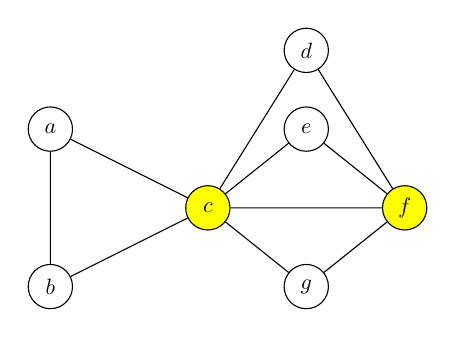
\begin{tikzpicture}[main_node/.style={circle,draw,minimum size=2em,inner sep=1, scale=0.8]}]
    \node[main_node] (1) at (-2, 1) {$a$};
    \node[main_node] (2) at (-2, -1)  {$b$};
    \node[main_node, fill=yellow] (3) at (0, 0) {$c$};
    \node[main_node] (4) at (1.25, 2)  {$d$};
    \node[main_node] (5) at (1.25,1) {$e$};
    \node[main_node, fill=yellow] (6) at (2.5,0) {$f$};
    \node[main_node] (7) at (1.25,-1)  {$g$};
    \draw (3) -- (1) -- (2) -- (3) -- (4) -- (6) -- (5) -- (3) --(6) -- (7) -- (3) -- (1);
\end{tikzpicture}

\caption{Graf $G$ iz primera~\ref{primerLema7}}
\label{fig:primerLema7graf}
\end{figure}
\end{primer}

\begin{lema}\label{Lema8}
Naj bo $G$ kograf dobljen s spojem grafov $G_1$ in $G_2$, kjer je $G_1$ nepovezan graf s komponentami $U_1, \dots, U_l$, $l \geq 2$, in  $V(G_2) = \{x\}$. Tedaj velja $\gamma_s(G) = Q(G, G_1)$.
\end{lema}
\begin{proof}
Sprva privzemimo, da ne obstaja tak $i, i \in [l]$, da bi imel graf $U_i$ lastnost $\mathcal{P^*}$. Po lemi~\ref{Lema7} sledi, da obstaja $\gamma_s$-množica $S$, da velja $x\in S$ in $|S \cap V(U_i)| = \gamma(U_i)$ za vsak $i \in [l]$. Množica $S$ je zato sestavljena iz vozlišča $x$ ter vsote vozlišč $S$ po posameznih komponentah $U_i$, to je $$\gamma_s(G) = 1 + \sum\limits_{i=1}^l\gamma(U_i).$$ Ker nobena komponenta nima lastnosti $\mathcal{P^*}$, je zgornja vsota enaka $Q(G, G_1)$, torej velja $\gamma_s(G) = Q(G, G_1)$.

Privzemimo sedaj, da ima neka komponenta $U_j$ lastnost $\mathcal{P^*}$. Po lemi~\ref{Lema7} obstaja $\gamma_s$-množica $S$, v kateri je vsebovan tudi $x$ in velja $|S \cap V(U_i)| \leq \gamma(U_i)$ za vsak $i \in [l]$. Recimo, da obstajata dve različni komponenti $U_k$ in $U_{k'}$, da za njiju velja  $|S \cap V(U_k)| < \gamma(U_k)$ in $|S \cap V(U_{k'})| < \gamma(U_{k'})$, kar pomeni, da so znotraj množice $U_k$ oziroma $U_{k'}$ taka vozlišča, ki niso dominirana z vozlišči iz množice $S \cap V(U_k)$ oziroma $S \cap V(U_{k'})$. Označimo dve taki vozlišči z $u_1\in V(U_k)$ in $u_2 \in V(U_{k'})$. Ker sta vsak v svoji komponenti, med njima ni povezave, sta pa obe dominirani (in varovani) le z vozliščem $x$. Po posledici~\ref{Observation1ii} sledi, da sta del klike in zato sosedne, kar pa vodi do protislovja. Torej lahko obstaja največ ena komponenta $U_k$, ki zadošča neenakosti $|S \cap V(U_k)| < \gamma(U_k)$.

Opazujmo sedaj število vozlišč množice $S$ v posameznih komponentah $U_i$ in jih primerjajmo z njihovim dominantnim številom. Po lemi~\ref{Lema7} velja, da sta števili enaki na vsaki komponenti, le na morebitni zgoraj opisani komponenti $U_k$ velja $|S \cap V(U_k)| = \gamma(U_k) - 1$. Ker je v množici $S$ zaradi leme~\ref{Lema6} tudi vozlišče $x$, ki ne leži v nobeni od komponent $U_i$, je kardinalnost množice $S$ kvečjemu večja ali enaka od seštevka dominantnih množic. Sledi $$Q(G, G_1) = \sum\limits_{i = 1}^l\gamma(U_i) \leq \gamma_s(G).$$

Za dokaz leme moramo pokazati, da v resnici velja enakost, torej $\sum_{i = 1}^l\gamma(U_i) = \gamma_s(G)$, pri tem pa z $D(U_i)$ označimo $\gamma$-množico za $U_i$. Ker ima $U_j$ lastnost $\mathcal{P^*}$, ločimo dva primera.
\begin{enumerate}[label=($\roman*$)]
\item $V(U_j)$ je klika. Definirajmo $$S' = \{x\} \bigcup\limits_{i = 1, i \neq j}^l D(U_i).$$
Množica $S'$ je dominantna množica, za varnostno dominacijo pa preverimo varovanje poljubnega vozlišča $v \in V(G) \setminus S'$, ki leži v enem od $U_i$.

Če velja $i\neq j$, obstaja vozlišče $u \in D(U_i)$, da velja $uv \in E(G)$. Ker je vozlišče $x \in S'$ in je sosedno vsem vozliščem iz množice $U_i$, je množica $(S' \setminus \{u\}) \cup\{v\}$ tudi dominantna množica.

V primeru $i=j$ je množica $S' \cap U_i$ prazna, zato za varovanje vozlišča $v$ izberemo vozlišče $x$. Množica $(S' \setminus \{x\}) \cup \{v\}$ je dominantna, saj $v$ dominira $V(G_2) = \{x\}$ in komponento $U_j$, ostala vozlišča pa so dominirana z vozlišči iz množice $\bigcup_{i = 1, i \neq j}^l D(U_i)$. Množica $S'$ je zato varnostnodominantna množica. Opazimo, da velja $$|S'| = \sum_{i=1, i\neq j}^l|D(U_i)|+ 1= \sum_{i=1}^l\gamma(U_i).$$

\item $\gamma(U_j) = 2$ in obstaja tako vozlišče $w \in V(U_j)$, da je množica $V(U_j) \setminus N_{U_j}[w]$ klika. Definirajmo $$S' = \{x, w\} \bigcup\limits_{i = 1, i \neq j}^l D(U_i).$$Opazimo, da je $S'$ dominantna množica, saj unija dominantnih množic dominira komponente $U_i$ za $i \neq j$, vozlišče $w$ svojo soseščino, vozlišče $x$ pa še preostala vozlišča iz klike $V(G) \setminus N_{U_j}[w]$. Za varnostno dominacijo je treba preveriti varovanje poljubnega vozlišča $v \in V(G) \setminus S'$, ki očitno leži v enem izmed $U_i$.

Če velja $i\neq j$, obstaja vozlišče $u \in D(U_i)$, da velja $uv \in E(G)$. Ker je $x \in S'$ in je soseden vsem vozliščem iz množice $U_i$, je množica $(S' \setminus \{u\}) \cup\{v\}$ tudi dominantna množica.

Če $i=j$ in obstaja povezava $vw \in E(G)$, potem je množica $(S' \setminus \{w\}) \cup \{v\}$ dominantna, saj unija dominantnih množic iz definicije $S'$ dominira komponente $U_i$ za $i\neq j$, vozlišče $x$ pa komponento $U_j$. Če $v$ in $w$ nista sosedni, pa vozlišče $v$ varuje $x$. Množica $(S' \setminus \{x\}) \cup \{v\}$ je namreč dominantna, saj velja $v \in V(U_j) \setminus N_{U_j}[w]$, ki je klika, torej jo $v$ dominira, vozlišče $w$ pa pokrije preostanek komponente $U_j$, ki je ravno zaprta soseščina vozlišča $w$. Tako smo dokazali, da je $S'$ varnostnodominantna množica za graf $G$, opazimo pa še, da velja$$|S'| = \sum_{i=1, i\neq j}^l|D(U_i)|+ 2= \sum_{i=1}^l\gamma(U_i).$$
\end{enumerate}
V obeh primerih smo dobili množico, ki je po kardinalnosti enaka seštevku posameznih dominantnih števil na komponentah $U_i$ za $i \in [l]$. Ker je $\gamma_s$-množica kvečjemu manjša od množice $S'$, velja neenakost $$\gamma_s(G) \leq \sum\limits_{i = 1}^l\gamma(U_i)  = Q(G, G_1).$$
Sledi, da velja $\gamma_s(G)  = Q(G, G_1)$.
\end{proof}

Zadnja pomembna lema podaja potrebne in zadostne pogoje za $\gamma_s(G) = 3$ v primeru, da je graf $G$ dobljen kot spoj dveh poljubnih nepovezanih grafov in nima lastnosti $\mathcal{P}$. Za lažje razumevanje navedimo najprej dve pomožni lemi, ki dokazujeta zadosten pogoj leme~\ref{Lema11}. 

\begin{lema}\label{Lema9}
Naj bo graf $G$ tak graf, ki nima lastnosti $\mathcal{P}$ in ki je dobljen kot spoj dveh nepovezanih grafov $G_1$ in $G_2$. Če velja $Q(G, G_1) \leq 3$ ali $Q(G, G_2) \leq 3$, velja $\gamma_s(G) = 3$.
\end{lema}
\begin{proof}
Ker $G$ ni poln graf, velja $\gamma_s \geq 2$, in ker $G$ nima lastnosti $\mathcal{P}$, po lemi~\ref{Lema4} sledi $\gamma_s \geq 3$. Brez škode za splošnost privzemimo $Q(G, G_1) \leq 3$ in pokažimo, da obstaja taka varnostnodominantna množica $S$ za graf $G$, da velja $|S|=3$. Pri tem bomo zaradi definicije $Q(G, G_1)$ ločili dva primera glede na lastnost $\mathcal{P^*}$ komponent grafa $G_1$, pri tem pa komponente grafa $G_1$ označimo z $U_1, \dots, U_l$.
\begin{enumerate}[label=($\roman*$)]
\item Nobena komponenta grafa $G_1$ nima lastnosti $\mathcal{P^*}$.

Po definiciji tedaj velja $Q(G, G_1) = 1 + \sum\limits_{i=1}^l \gamma(U_i) = 1 + \gamma(G_1)$. Ker je $G_1$ nepoln graf, velja $\gamma(G_1) \neq 1$, zato iz $Q(G, G_1) \leq 3$ sledi $\gamma(G_1) = 2$. Naj bo $\{y, z\}$ dominantna množica za graf $G_1$ in naj bo $S=\{x, y,  z\}, x \in V(G_2)$, množica, za katero bi radi pokazali, da je varnostnodominantna. Ker je $\{y, z\} \subset S$, je tudi $S$ dominantna množica. Naj bo $v \in V(G_1) \setminus S$ poljubno vozlišče.

Če $v$ leži v podgrafu $G_2$, zaradi lastnosti spoja velja $yv \in E(G)$. Ker vozlišče $z$ leži v $G_1$, $v$ pa v $G_2$, je zaradi lastnosti spoja tudi množica $(S \setminus \{y\}) \cup \{v\}$ dominantna množica za $G$, torej $y$ varuje vozlišče $v$.

Če se $v$ nahaja v podgrafu $G_1$, gotovo obstaja povezava $yv \in E(G_1)$ ali $zv \in E(G_1)$, saj je $\{y, z\}$ dominantna množica grafa $G_1$. Če velja $yv \in E(G_1)$, je $(S \setminus \{y\}) \cup \{v\}$ dominantna množica, saj $y$ in $v$ ležita v $G_1$, vozlišče $x$ pa v $G_2$. To pomeni, da vozlišče $y$ varuje vozlišče $v$. Podobno lahko premislimo, da je vozlišče $v$ v primeru $zv \in E(G_1)$ varovano z vozliščem $z$. Ker smo obravnavali vse možnosti, sledi, da je $S$ varnostnodominantna množica.

\item Obstaja komponenta $U_j$ grafa $G_1$, ki zadošča lastnosti $\mathcal{P^*}$.

Najprej privzemimo, da je komponenta $U_j$ poln podgraf. Ker velja $Q(G, G_1) = \sum\limits_{i=1}^l \gamma(U_i) \leq 3$ in $\gamma(U_j) = 1$, sledi $\gamma(G_1 \setminus V(U_j)) \leq 2$. Naj bo $S = \{x, y, z\}$, kjer je $x \in V(G_2)$, množica $\{y, z\}$ pa je dominantna množica grafa $G_1 \setminus V(U_j)$. Zaradi lastnosti spoja je $S$ dominantna množica, dokažimo pa, da je tudi varnostnodominantna. Naj bo vozlišče $v$ poljubno vozlišče iz množice $V(G) \setminus S$. Če velja $v \in V(U_j)$, je $(S \setminus \{x\}) \cup \{v\}$ dominantna množica, saj $v$ dominira množico $U_j \cup G_2$, vozlišči $y$ in $z$ pa dominirata $(G_1 \setminus U_j) \cup G_2$. Vozlišče $x$ torej varuje vozlišče $v$. Če $v \not\in V(U_j)$, po definiciji dominantne množice obstaja bodisi $yv \in E(G)$ bodisi $zv \in E(G)$. Brez škode za splošnost privzemimo  $yv \in E(G)$, kar pomeni, da je $v$ sosedne vsem vozliščem iz $G_2$, vozlišče $x$ pa vsem iz $G_1$, torej je množica $(S \setminus \{y\}) \cup \{v\}$ varnostnodominantna, vozlišče $y$ pa varuje $v$. Podobno v primeru $yz \in E(G)$ opazimo, da je vozlišče $v$ varovano z vozliščem $z$. Sledi, da je $S$ varnostnodominantna množica grafa $G$.

Privzemimo sedaj, da $U_j$ ni poln graf. Po definiciji lastnosti $\mathcal{P^*}$ tedaj velja $\gamma(U_j) = 2$, obstaja pa tudi tako vozlišče $w \in V(U_j)$, da je množica $V(U_j) \setminus N_{U_j}[w]$ klika. Ker je $G_1$ nepovezan graf, po definiciji funkcije $Q$ $$Q(G, G_1)= \sum\limits_{i=1}^l \gamma(U_i)$$ velja, da $Q(G, G_1) \geq 3$. Če rezultat združimo s predpostavko, sledi enakost $Q(G, G_1) = 3$. Iz tega sledi, da ima $G_1$ natanko dve komponenti $U_1$ in $U_j$, za $U_1$ pa velja $\gamma(U_1)=1$. Označimo s $S$ množico $\{x, y, w\}$, kjer je $x\in V(G_2)$, množica $\{y\}$ dominantna množica komponente $U_1$ in $w$ vozlišče iz definicije lastnosti $\mathcal{P^*}$. Ker je graf $G$ spoj grafov $G_1$ in $G_2$, množica $S$ pa ima predstavnika tako v $G_1$ in $G_2$, je množica $S$ dominantna množica. Za varnostno dominacijo si oglejmo varovanje poljubnega vozlišča $v \in V(G) \setminus S$. Če $v$ leži v množici $V(U_1) \cup V(G_2)$, je množica $(S \setminus \{y\}) \cup \{v\}$ dominantna množica, saj velja $w\in G_1$ in $x \in G_2$. Vozlišče $y$ torej varuje vozlišče $v$. Če se $v$ nahaja v množici $U_j$ in obstaja povezava $vw \in E(G_1)$, vozlišče $w$ varuje $w$; v dominantni množici sta tako $x\in G_1$ kot tudi $y \in G_2$, zaradi lastnosti spoja grafa pa je množica $(S \setminus \{w\}) \cup \{v\}$ dominantna. Če povezave med vozliščema $v$ in $w$ ni, vozlišče $v$ leži v $V(U_j) \setminus N_{U_j}[w]$. Tedaj vozlišče $v$ varuje $x$, saj je $V(U_j) \setminus N_{U_j}[w]$ klika in posledično je $(S \setminus \{x\}) \cup \{v\}$ dominantna množica.
 \end{enumerate}
Obravnavali smo vse možnosti za $Q(G, G_1) \leq 3$ in pokazali, da iz vseh sledi $\gamma_s(G) = 3$. Podobno lahko pokažemo, da iz  $Q(G, G_2) \leq 3$ sledi $\gamma_s(G) = 3$.
 \end{proof}
 
 \begin{lema}\label{Lema10}
 Naj bo $G$ kograf, ki nima lastnosti $\mathcal{P}$ in je dobljen s spojem nepovezanih grafov $G_1$ in $G_2$. Če velja $\gamma_s(G_1) = 3$ ali $\gamma_s(G_2) = 3$, tedaj velja $\gamma_s(G) = 3$.
 \end{lema}
 \begin{proof}
 Ker sta $G_1$ in $G_2$ nepovezana grafa, graf $G$ ni poln, zato velja $\gamma_s(G) \neq 1$. Ker $G$ nima lastnosti $\mathcal{P}$, po lemi~\ref{Lema4} velja $\gamma_s(G) \neq 2$, zato velja $\gamma_s(G) \geq 3$. Najprej privzemimo, da velja predpostavka $\gamma_s(G_1) = 3$, množica $S = \{x, y, z\}$ pa naj bo $\gamma_s$-množica za graf $G_1$. Pokažimo, da je $S$ $\gamma_s$-množica tudi za graf $G$.
 
Opazimo, da je množica $S$ dominantna množica za graf $G$, saj je $\gamma_s$-množica za graf $G_1$, zaradi lastnosti $G = G_1 + G_2$ pa dominira tudi celoten $G_2$. Vzemimo sedaj poljubno vozlišče $v \in V(G) \setminus S$. Če velja $v \in V(G_2)$, vozlišče $v$ varujejo vsa tri vozlišča $x, y, z$. Če velja $v \in V(G_1)$, v množici vozlišč $V(G_1)$ obstaja vozlišče $u \in \{x, y, z\}$ iz $S$, ki ga varuje, saj je $S$ $\gamma_s$-množica za graf $G_1$. Ker je $(S \setminus \{u\}) \cup \{v\}$ dominantna množica v $G_1$, je zaradi spoja dominantna tudi v $G$. Množica $S$ je zato $\gamma_s$-množica grafa $G$ in velja $\gamma_s(G) = 3$. Podobno se prepričamo, da iz $\gamma_s(G_2) = 3$ sledi $\gamma_s(G) = 3$. 
 \end{proof}
 
 Dokažimo sedaj, da implikacija v obeh lemah velja tudi v obratno smer.
 
 \begin{lema}\label{Lema11}
 Naj bo $G$ kograf, ki nima lastnosti $\mathcal{P}$ in ki je dobljen s spojem nepovezanih grafov $G_1$ in $G_2$. Tedaj velja $\gamma_s(G) = 3$ natanko tedaj, ko drži eden izmed naslednjih dveh pogojev:
\begin{enumerate}[label=($\roman*$)]
\item $Q(G, G_1) \geq 3$ ali $Q(G, G_2) \geq 3$.
\item $\gamma_s(G_1) = 3$ ali $\gamma_s(G_2) = 3$.
\end{enumerate}
 \end{lema}
 
 \begin{proof}
$(\Leftarrow)$ Sledi iz lem~\ref{Lema9} in~\ref{Lema10}.

\medskip
$(\Rightarrow)$ Privzemimo, da velja $\gamma_s(G) = 3$ in naj bo $S$ $\gamma_s$-množica grafa $G$. Dokaz bomo razdelili na tri dele glede na to, v katerem grafu $G_1$ in $G_2$ se vozlišča množice $S$ nahajajo in glede na lastnosti $\mathcal{P^*}$ komponent grafov $G_1$ in $G_2$.
\begin{itemize}
\item $|V(G_1) \cap S| = 3$ ali $|V(G_2) \cap S| = 3$.

Brez škode za splošnost privzemimo $|V(G_1) \cap S| = 3$. Očitno je množica $S$ varnostnodominantna množica tudi za graf $G_1$, pokažimo pa, da je tudi minimalna. Ker je graf $G_1$ nepovezan, sledi $\gamma_s(G_1) \geq 2$. Recimo, da bi obstaja $\gamma_s$-množica $S' = \{x,y\}$ grafa $G_1$. Izberimo poljubno vozlišče $z$ grafa $G_2$. Opazimo, da je množica $(S' \setminus \{y\}) \cup \{z\}$ dominantna množica za graf $G$, iz česar sledi, da je $S'$ varnostnodominantna množica grafa $G$, kar vodi v protislovje s predpostavko $\gamma_s(G) = 3$. Sledi torej, da velja $\gamma_s(G_1) = 3$. Podobno v primeru $|V(G_2) \cap S| = 3$ sledi, da velja $\gamma_s(G_2) = 3$, kar je natanko točka $(i)$ leme, ki jo dokazujemo.

\item $|V(G_1) \cap S| \neq 3$ in $|V(G_2) \cap S| \neq 3$.

Ker množica $S$ po predpostavki vsebuje tri vozlišča, sta možni delitvi vozlišč v graf $G_1$ in $G_2$ ali kot $|V(G_1) \cap S| = 1$ in $|V(G_2) \cap S| = 2$ ali kot $|V(G_1) \cap S| = 2$ in $|V(G_2) \cap S| = 1$. Brez škode za splošnost se omejimo na primer $|V(G_1) \cap S| = 2$ in $|V(G_2) \cap S| = 1$ in pokažimo, da velja $Q(G, G_1) \leq 3$. Ker je za izračun $Q(G, G_1)$ bistvena lastnost $\mathcal{P^*}$ komponent $G_1$, obravnavajmo dva primera: ko obstaja komponenta grafa $G_1$ z lastnostjo $\mathcal{P^*}$ in ko taka komponenta ne obstaja.
\begin{itemize}
\item Nobena komponenta grafa $G_1$ nima lastnosti $\mathcal{P^*}$.

Vrednost $Q$ se tedaj izračuna kot $$Q(G, G_1) = 1 + \sum\limits_{i=1}^l \gamma(U_i),$$ kjer so $U_i$ komponente grafa $G_1$. Za dokaz neenakosti $Q(G, G_1) \leq 3$ je zato dovolj, da dokažemo neenakost $\gamma(G_1) \leq 2$. Ker je $G_1$ nepovezan graf, sledi, da velja $\gamma(G_1) \geq 2$, zato privzemimo $\gamma(G_1) > 2$ in pokažimo, da nas to pripelje do protislovja. Naj bosta $y$ in $z$ vozlišči iz množice $V(G_1) \cap S$, vozlišče $x$ pa edini element množice  $V(G_2) \cap S$. Zaradi predpostavke $\gamma(G_1) > 2$ opazimo, da množica $\{y, z\}$ ni dominantna množica za graf $G_1$. Kakor v posledici~\ref{Observation1ii} z $A$ označimo množico vozlišč grafa $G_1$, ki so dominirani le z vozliščem $x$, to pomeni $$A = V(G_1) \setminus (N_{G_1}[y] \cup N_{G_1}[z] ).$$ Ker $\{y, z\}$ ni dominantna množica, je $A$ neprazna množica, po posledici~\ref{Observation1ii} pa tudi klika. Graf $G_1$ je po predpostavki nepovezan graf in ker je množica $A$ klika, leži v celoti v eni od komponent, označimo jo z $U_1$, grafa $G_1$. Če vozlišči $y$ in  $z$ ne ležita v komponenti $U_1$, velja $V(U_1) = A$, to pa je v protislovju s predpostavko, da nobena komponenta grafa $G_1$ nima lastnosti $\mathcal{P^*}$, saj ima poln graf vedno lastnost $\mathcal{P^*}$. Zato zdaj privzemimo, da $y \in V(U_1)$. Če je v komponenti $U_1$ tudi vozlišče $z$, je v $C_1$ tudi njuna soseščina $N_{G_1}[y] \cup N_{G_1}[z]$, kar pomeni, da $V(G_1) = V(U_1)$, kar je v protislovju z nepovezanostjo grafa $G_1$. Zato mora vozlišče $z$ ležati v drugi komponenti, ki jo označimo z $U_2$. Izberimo poljubno vozlišče $u \in V(U_1)$. Če povezava $uy$ ne obstaja --povezava $uz$ pa ne obstaja, ker vozlišči ležita v različnih komponentah--, vozlišče $u$ leži v množici $A$. To pomeni, da je $\gamma(U_1) = 2$, obstaja pa vozlišče $y \in V(U_1)$, da je $V(U_1) \setminus N_{U_1} [y]$ klika, kar je po definiciji lastnost $\mathcal{P^*}$ podgrafa $U_1$. S tem smo prišli v protislovje, kar pomeni, da smo dokazali $\gamma(G_1) = 2$ in posledično $Q(G, G_1) \leq 3$.

\medskip
\item Obstaja komponenta $U_j$ grafa $G_1$, ki ustreza lastnosti $\mathcal{P^*}$.

Sprva privzemimo, da je $U_j$ poln graf. Zaradi lastnosti $\mathcal{P^*}$ je vrednost $Q$ enaka $Q(G, G_1) = \sum\limits_{i=1}^l \gamma(U_i)$, zato je za neenakost $Q(G, G_1) \leq 3$ dovolj pokazati, da velja $\gamma(G_1 \setminus V(U_j)) \leq 2$. Zopet se dokazovanja lotimo s protislovjem, zato privzemimo, da velja $\gamma(G_1 \setminus V(U_j)) > 2$, kar pomeni, da velja $\gamma(G_1) > 3$. Naj bosta $y$ in $z$ vozlišči iz množice $V(G_1) \cap S$, vozlišče $x$ pa edini element množice  $V(G_2) \cap S$. Po predpostavki $\gamma(G_1) > 3$ množica $\{y, z\}$ ne more biti dominantna množica. Izberimo poljubno vozlišče $v \in V(G_1) \setminus (N_{G_1}[y] \cup N_{G_2}[z])$. Ker je $S$ $\gamma_s$-množica, vozlišče $v$ pa ni sosedno niti z vozliščem $y$ niti s $z$, je vozlišče $v$ varovano z vozliščem $x$. To pomeni, da je množica $\{v, y, z\}$ dominantna množica grafa $G_1$, kar nasprotuje predpostavki $\gamma(G_1) > 3$. Sledi, da velja $\gamma(G_1 \setminus V(U_j)) \leq 2$.

\medskip
Privzemimo sedaj, da $U_j$ ni poln graf. Po definiciji lastnosti $\mathcal{P^*}$ sledi, da velja $\gamma(U_j) = 2$, obstaja pa tudi vozlišče $w \in V(U_j)$, da je $V(U_j) \setminus N_{U_j}[w]$ poln graf. Ker je $Q(G, G_1) = \sum\limits_{i=1}^l \gamma(U_i)$ in $\gamma(U_j) = 2$, sledi $Q(G, G_1) \geq 3$, zato je za dokaz enakosti $Q(G, G_1) = 3$ dovolj pokazati enakost $\gamma(G \setminus V(U_j)) = 1$. Zopet naj bosta $y$ in $z$ vozlišči iz množice $V(G_1) \cap S$, vozlišče $x$ pa edini element množice  $V(G_2) \cap S$. 

Najprej si oglejmo primer, ko velja $y, z \in V(U_j)$. Naj bo vozlišče $v$ poljubno vozlišče iz množice $V(G_1) \setminus V(U_j)$. Ker je $S$ $\gamma_s$-množica za $G$, vozlišči $z$ in $y$ pa obe pripadata komponenti $U_j$, je vozlišče $v$ varovano z vozliščem $x$. To pomeni tudi, da je množica $\{v, y, z\}$ dominantna množica grafa $G$. Ker se $v$ nahaja v drugi komponenti kot $y$ in $z$, pomeni, da $v$ dominira celoten graf $V(G) \setminus V(U_j)$, zato sledi $\gamma(G_1 \setminus V(U_j)) = 1$.

V primeru, da $y, z \not\in U_j$, je celotna komponenta $U_j$ varovana le z vozliščem $x$. Po posledici~\ref{Observation1ii} sledi, da je $U_j$ poln graf in velja $\gamma(U_j) = 1$, kar pa je v protislovju s predpostavko $\gamma(U_j) = 2$. Zato eno vozlišče množice $\{y, z\}$ zagotovo leži v komponenti $U_j$. Brez škode za splošnost recimo, da je to vozlišče $y$. Izberimo poljubno vozlišče $u \in V(U_j)$, ki ni sosedne vozlišču $y$. Tako vozlišče zagotovo obstaja, saj bi sicer veljalo $\gamma(U_j) = 1$. Ker se $u$ nahaja v drugi komponenti kot $z$ in ni sosedne vozlišču $y$, ga po definiciji varnostne dominacije lahko varuje le vozlišče $x$. Sledi, da je množica $\{u, y, z\}$ dominantna množica, in ker vozlišči $y$ in $u$ ležita v komponenti $U_j$, vozlišče $z$ dominira preostanek grafa. Zaključimo, da velja enakost $\gamma(G_1 \setminus V(U_j)) = 1$.
\end{itemize}
\end{itemize}
 \end{proof}
 
 \subsection{Algoritem PJB}
 
\begin{algorithm}[h!]
\caption{Algoritem PJB: Varnostna dominacija na kografih}\label{alg:pradhan}
\begin{algorithmic}[1]
\Function{izračunajGamaS}{graf $G$}
\State izračun $T_G$
\State $(c_1, c_2, ..., c_r)$ $\leftarrow$ BFS kodrevesa $T_G$
\For {($i = 1$ to $r$)}
	\If {$c_i$ je list}
    	\State $\gamma_s(T_G(c_i))$  $\leftarrow$ 1
    \Else
    	\State ($u_1$, $u_2$, ... , $u_l$) $\leftarrow$ potomci $c_i$
        \If {$c_i$ ima oznako $\cup$}
        	\State $\gamma_s(T_G(C_i)) \leftarrow \sum\limits_{j=1}^l \gamma_s(T_G(u_j))$
          \Else  \hfill\Comment{$c_i$ ima oznako $+$}
             \If {vsak $u_i$ je list}
             	\State $\gamma_s(T_G(c_i)) \leftarrow 1$
             \ElsIf {$T_G(c_i)$ ima lastnost $\mathcal{P}$}
             	\State $\gamma_s(T_G(c_i)) \leftarrow 2$
             \ElsIf {$l \geq 3$}
                 \State $\gamma_s(T_G(c_i)) \leftarrow 3$
             \ElsIf {$c_i$ ima dva potomca, kjer je $u_1$ list,  $u_2$ pa ni list}
                  	\State $\gamma_s(T_G(c_i)) \leftarrow Q(T_G(c_i), T_G(u_2))$
               \ElsIf {$c_i$ nima lista za potomca}
                  		\If {$\gamma_s(T_G(u_1)) = 3$  ali $\gamma_s(T_g(u_2)) = 3$ \\ \hspace{100px} ali $Q(T_G(c_i), T_G(u_1)) \leq 3$  ali $Q(T_G(c_i), T_G(u_2)) \leq 3$}
                    		\State $\gamma_s(T_G(c_i)) \leftarrow 3$
                    	\Else
                    		\State $\gamma_s(T_G(c_i)) \leftarrow 4$
                    	\EndIf
                  \EndIf
                \EndIf
            \EndIf
\EndFor
\State \textbf{return} $\gamma_s(G) = \gamma_s(T_G(c_r))$
\EndFunction
\end{algorithmic}
\end{algorithm}

Za izračun $\gamma_s(G)$ se omejimo na povezane grafe, sicer s pomočjo formule v vrstici 10 algoritma~\ref{alg:pradhan} izračunamo število $\gamma_s$ za vsako od povezanih komponent grafa. Najprej izračunamo pripadajoče kodrevo $T_G$ grafa $G$ ter njegova vozlišča uredimo---zaporedje vozlišč $\sigma = (c_r, c_{r-1}, ..., c_1)$ dobimo z iskalnim algoritmom BFS (iskanje v širino), uporabimo pa njegov obrat $\sigma ^{-1} = (c_1, ..., c_r)$, saj na ta način zagotovimo, da vsako vozlišče v zaporedju nastopi pred svojim staršem v drevesni strukturi. Algoritem bo namreč na $i$-ti iteraciji izračunal $\gamma_s$ grafa $T_G(c_i)$, za izračun pa potrebuje vrednosti potomcev vozlišča $c_i$, zato morajo biti v $i$-ti iteraciji te že izračunane.

S pomočjo zanke se sprehodimo čez vsa vozlišča $c_i$ našega zaporedja ter izračunamo $\gamma_s(T_G(c_i))$, pri čemer obravnavamo različne primere, ki smo jih v prejšnjem poglavju izpeljali s pomočjo naštetih lem. Pri obravnavi potomce vozlišča $c_i$ označimo z $u_1, ..., u_l$. Vsakemu vozlišču, ki je list, po trditvi~\ref{theorem3.3} dodelimo vrednost $1$. Če je  $c_i$ notranje vozlišče kodrevesa $T_G$ in ima oznako $\cup$, vrednost $\gamma_s(T_G(c_i))$ po posledici~\ref{vecUnij} dobimo s seštevkom $\gamma_s(T_G(u_j))$ za vsak $u_j$, saj gre za nepovezan graf, kjer se $\gamma_s$ sešteje po komponentah za povezanost. Če je $c_i$ notranje vozlišče z oznako $+$, je graf $T_G(c_i)$ dobljen s spojem grafov $T_G(u_1), \dots , T_G(u_l)$, izračun $\gamma_s(T_G(c_i))$ pa je odvisen od lastnosti vozlišč $u_1, \dots, u_l$:
\begin{itemize}
\item Vsako vozlišče $u_i$ je list: graf $T_G(c_i)$ je očitno poln graf, zato po trditvi~\ref{theorem3.3} sledi $\gamma_s(T_G(c_i)) = 1$. 
\item Obstaja vozlišče $u_i$, ki ni list: graf $T_G(c_i)$ potem ni poln graf, torej velja $\gamma_s(T_G(c_i)) \geq 2$. S pomočjo preverjanja naslednjih lastnosti lahko določimo natančno vrednost $\gamma_s(T_G(c_i))$:
\begin{itemize}
\item Če ima $T_G(c_i))$ lastnost $\mathcal{P}$, iz leme~\ref{Lema4} sledi $\gamma_s(T_G(c_1)) = 2$.
\item Če $T_G(c_i))$ nima lastnosti $\mathcal{P}$ in ima $c_i$ vsaj tri potomce, po lemi~\ref{Lema5} sledi $\gamma_s(T_G(c_i)) = 3$.
\item Če $T_G(c_i))$ nima lastnosti $\mathcal{P}$ in ima $c_i$ natanko dva potomca, kjer je en izmed njiju list, po lemi~\ref{Lema8} sledi $\gamma_s(T_g(c_i)) = Q(T_G(c_i), T_G(u_1))$, kjer je $u_1$ tisti potomec vozlišča $c_i$, ki ni list.
\item Če $T_G(c_i))$ nima lastnosti $\mathcal{P}$ in ima $c_i$ natanko dva potomca, ki sta notranji vozlišči, po lemi~\ref{Lema11} izračunamo $\gamma_s(T_G(c_i))$: če velja ali $Q(G, G_1) \geq 3$ ali $Q(G, G_2) \geq 3$ ali $\gamma_s(G_1) = 3$ ali $\gamma_s(G_2) = 3$, velja $\gamma_s(T_G(c_i)) = 3$, sicer velja $\gamma_s(T_G(c_i)) = 4$.
\end{itemize}
\end{itemize}

\begin{izrek} Algoritem~\ref{alg:pradhan} pravilno izračuna varnostnodominantno število za poljuben kograf $G$ v času $O(m(G) + n(G))$.
\end{izrek}
\begin{proof}
Pravilnost algoritma smo upravičili z lemami iz prejšnjega poglavja, zanima pa nas tudi časovna zahtevnost algoritma.

Naj bo $G$ graf z $n$ vozlišči in $m$ povezavami. Kodrevo $T_G$ lahko konstruiramo v $O(n(G)+m(G))$ času \cite{corneil1985linear}. Algoritem BFS potrebuje $O(|V(T_G)| + |E(T_G)|)$ časa za ureditev vozlišč $G$. Pri računanju $\gamma_s(T_G(c_i))$ na $i$-tem koraku algoritma opravimo izračune različnih vrednosti (lastnost $\mathcal{P}$, $Q(T_G(c_i), T_G(u))$, $\gamma(T_G(c_i))$, ...):
\begin{itemize}
\item Izračun $\gamma(T_G(c_i))$.

Pri izračunu $Q(T_G(c_i), T_G(u))$ potrebujemo tudi dominantna števila komponent grafa $T_G(c_i))$. Za vozlišča $c_i$, ki so listi, očitno velja $\gamma(T_G(c_i)) = 1$. V primeru unije velja enačba iz  posledice~\ref{vecUnij}: $$\gamma(T_G(c_i)) = \sum\limits_{i=1}^l \gamma(T_G(u_i)),$$v primeru spoja pa posplošimo rezultat iz izreka~\ref{theorem4.6}; če je kateri od potomcev $c_i$ list, velja $\gamma(T_G(c_i)) = 1$, sicer velja $\gamma(T_G(c_i)) = 2$. Izračun dominantnega števila tako potrebuje $O(|N_{T_G(ci)}(c_i)|)$ časa.

\item Lastnost $\mathcal{P}$, lastnost $\mathcal{R}$, lastnost $\mathcal{P^*}$.

Za izračun naštetih lastnosti uvedemo tri sezname dolžine $|V(T_G)|$: $\mathcal{R}$, $\mathcal{A^*}$ in $\mathcal{R^*}$, ki jih na začetku nastavimo na $\mathcal{R}[v]=\mathcal{A^*}[v]=\mathcal{R^*}[v]=0$ za vsak $v\in T_G$.

Seznam $\mathcal{R}$ bo beležil vozlišča z lastnostjo $\mathcal{R}$, zato ga za trenutno vozlišče $c_i$ nastavimo na $\mathcal{R}[{c_i}]=1$, če ima $c_i$ oznako $\cup$, ima natanko dva potomca $x$ in $y$ ter velja $\gamma(T_G(x)) = 1$ ter $\gamma_s(T_G(y)) = 1$.

Seznam $\mathcal{A^*}$ ustreza lastnosti $\mathcal{P^*}$; za vozlišče $c_i$ nastavimo $\mathcal{A}^*[{c_i}]=1$, če je $c_i$ list ali vozlišče z oznako $+$ in izpolnjuje pogoje iz leme ~\ref{Lema3}: $\gamma_s(T_G(c_i)) = 1$ ali vozlišče $c_i$ ima za potomca vozlišče z lastnostjo $\mathcal{R}$ in noben potomec vozlišča $c_i$ ni list.

Seznam $\mathcal{R^*}$ nam omogoča hitro računanje $Q(T_G(c_i), T_G(u))$, saj za vozlišč $c_i$ nastavimo $\mathcal{R^*}[c_i] = 1$, če ima $c_i$ potomca $u_j$ z lastnostjo $\mathcal{P^*}$, to je $\mathcal{A^*}[u_j] = 1$.

Hitro se prepričamo, da za posodobitev seznamov $\mathcal{R}$, $\mathcal{A^*}$ in $\mathcal{R^*}$ na $i$-ti iteraciji potrebujemo $O(|N_{T_G(c_i)}(c_i)|)$ časa.

\item Izračun $\gamma_s(T_G(c_i))$.

Če je $c_i$ list, velja $\gamma_s(T_G(c_i)) = 1$. Če ima $c_i$ oznako $\cup$, velja $$\gamma_s(T_G(c_i)) = \sum\limits_{j=1}^l \gamma_s(T_G(u_j)),$$ kar napravimo v $O(|N_{T_G(c_i)}(c_i)|)$ časa.V primeru, da je $c_i$ vozlišče z oznako $+$, algoritem najprej preveri, če so vsa vozlišča listi ($O(|N_{T_G(ci)}(c_i)|)$). Sicer nadalje preveri, ali ima $c_i$ lastnost $\mathcal{P}$. Po lemi~\ref{Lema2} je dovolj preveriti le potomce $c_i$, če so ali listi ali vozlišča z lastnostjo $\mathcal{R}$ oziroma če so njihovi potomci polni grafi. To lahko hitro preverimo s pomočjo seznama $\mathcal{R}$ in vrednosti $\gamma_s$ za potomce vozlišča $c_i$, ki so že izračunane. Zaradi predhodne inicializacije seznama $\mathcal{R}$ in beleženja $\gamma_s$ na vsakem koraku se lastnost $\mathcal{P}$ lahko preveri v $O(|N_{T_G(ci)}(c_i)|)$ času.

Če $T_G(c_i)$ nima lastnosti $\mathcal{P}$, algoritem preveri število potomcev, kar ima prav tako časovno zahtevnost $O(|N_{T_G(ci)}(c_i)|)$. V primeru dveh potomcev, $u_1$ in $u_2$, algoritem izračuna $Q(T_G(c_i), T_G(u_j))$ za $j \in \{1, 2\}$ (odvisno od tega, če je en od njiju list), za to pa potrebuje informacijo o lastnosti $\mathcal{P^*}$ komponent grafa $T_G(u_j)$. Zaradi predhodne inicializacije seznama $\mathcal{R^*}$ za to porabimo konstanten čas, za izračun $Q(T_G(c_i), T_G(u_j))$ pa tako skupaj potrebujemo  $O(|N_{T_G(ci)}(c_i)|)$. 
\end{itemize}
Na $i$-ti iteraciji tako potrebujemo $O(|N_{T_G(ci)}(c_i)|)$ časa, da posodobimo sezname $\mathcal{R}$, $\mathcal{A^*}$ in $\mathcal{R^*}$ ter izračunamo $\gamma_s(T_G(c_i))$. Algoritem zato za izračun kodrevesa $T_G$ in izračun $\gamma_s(G)$  potrebuje $O(|V(T_G)| + |E(T_G)|)$ časa, zato je algoritem linearen.
\end{proof}

\begin{primer}
\begin{figure}[h!]
\centering
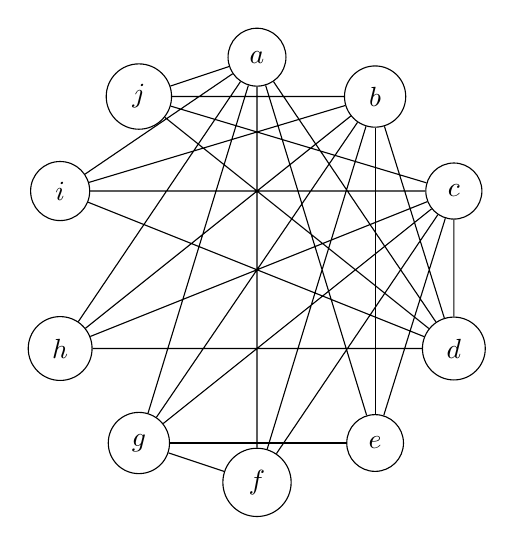
\begin{tikzpicture}[main_node/.style={circle,draw,inner sep=5pt, minimum size=5pt}]

   \node[main_node] (1) at (0, 2.7) {$a$};
    \node[main_node] (2) at (1.5, 2.2) {$b$};
    \node[main_node] (3) at (2.5, 1)  {$c$};
    \node[main_node] (4) at (2.5, -1) {$d$};
    \node[main_node] (5) at (1.5, -2.2)  {$e$};
    \node[main_node] (6) at (0, -2.7) {$f$};
    \node[main_node] (7) at (-1.5, -2.2) {$g$};
    \node[main_node] (8) at (-2.5, -1) {$h$};
    \node[main_node] (9) at (-2.5, 1)  {$i$};
    \node[main_node] (10) at (-1.5, 2.2) {$j$};
  
    \draw (1) -- (10) -- (2) -- (9) -- (3) -- (10) -- (4) -- (1) -- (9) -- (4) -- (2) -- (8) -- (1) -- (5) -- (3) -- (8) -- (4) -- (3) -- (6) -- (1) -- (7) -- (2) -- (6) -- (7) --(3) ;
    \draw (7) -- (5) -- (2) ;

\end{tikzpicture}
\caption{Kograf $G$, na katerem je bil zagnan algoritem PJB.}  \label{fig:skica-pradhan-graf}
\end{figure}

\begin{figure}[h!]
\centering
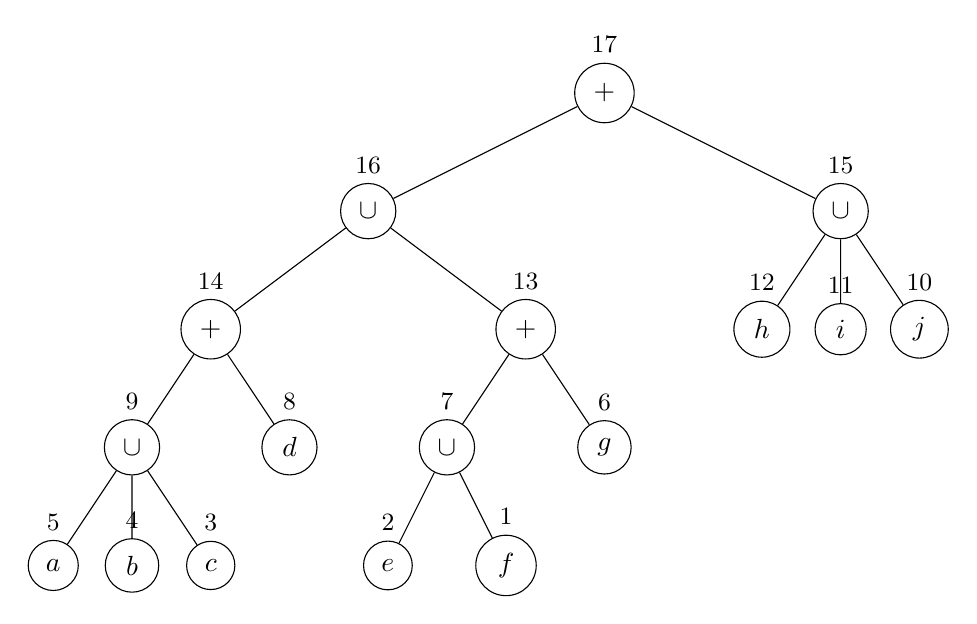
\begin{tikzpicture}[main_node/.style={circle,draw,inner sep=4pt, minimum size=4pt]}]
	\node[main_node, label=\small{5}] (5) at (-7, -2.5) {$a$};
	\node[main_node, label=\small{4}] (4) at (-6, -2.5) {$b$};
	\node[main_node, label=\small{3}] (3) at (-5, -2.5) {$c$};
	\node[main_node, label=\small{2}] (2) at (-2.75, -2.5) {$e$};
    \node[main_node, label=\small{1}] (1) at (-1.25, -2.5) {$f$};

	\node[main_node, label=\small{9}] (9) at (-6, -1) {$\cup$};
    \node[main_node, label=\small{8}] (8) at (-4, -1) {$d$};
    \node[main_node, label=\small{7}] (7) at (-2, -1)  {$\cup$};
    \node[main_node, label=\small{6}] (6) at (-0, -1) {$g$};
    
    \node[main_node, label=\small{14}] (14) at (-5, 0.5)  {$+$};
    \node[main_node, label=\small{13}] (13) at (-1, 0.5) {$+$};
    \node[main_node, label=\small{12}] (12) at (2, 0.5) {$h$};
    \node[main_node, label=\small{11}] (11) at (3, 0.5) {$i$};
    \node[main_node, label=\small{10}] (10) at (4, 0.5)  {$j$};
    
    \node[main_node, label=\small{16}] (16) at (-3, 2) {$\cup$};
    \node[main_node, label=\small{15}] (15) at (3, 2)  {$\cup$};
    
    \node[main_node, label=\small{17}] (17) at (0,3.5)  {$+$};

\draw (12) -- (15) -- (10);
\draw (11) --  (15) -- (17) -- (16) -- (13) -- (6);
\draw (2) -- (7) -- (1);
\draw (16) -- (14) -- (9) -- (5);
\draw (8) -- (14);
\draw (4) -- (9) -- (3);
\draw (13) -- (7);

\end{tikzpicture}
\caption{Kodrevo za graf $G$ s slike~\ref{fig:skica-pradhan-graf}, na katerem je bil zagnan algoritem PJB. Števila ob vozliščih označujejo obratni vrstni red vozlišč, kot jih uredi BFS algoritem.}  \label{skica pradhan}
\end{figure}
Na sliki~\ref{fig:skica-pradhan-graf} je graf $G$, na katerem zaženemo algoritem za iskanje $\gamma_s$. Najprej izračunamo njegovo kodrevo (na sliki~\ref{skica pradhan}), nato pa poženemo BFS algoritem in v obratnem vrstnem redu oštevilčimo vozlišča. Na $i$-ti iteraciji najprej posodobimo sezname $\mathcal{R}$, $\mathcal{P}^*$ in $\mathcal{R}^*$, nato pa izračunamo vrednost $\gamma_s(T_G(c_i))$ glede na zgoraj razdeljene primere. Iz zadnje vrstice tabele je razvidno, da velja $\gamma(G)=2$ in $\gamma_s(G)=3$. Primer dominantne množice sta množici $\{a,  h\}$ in  $\{g,d\}$, vendar nista varnostnodominantni, saj v prvem primeru ni varovano vozlišče $f$, v drugem primeru pa vozlišče $j$

Primer $\gamma_s$-množice je množica $\{a, g, d\}$, saj je množica $\{e, f, h, i, j\}$ varovana z vozliščem $a$, množica $\{b, c\}$ pa z vozliščem $g$.  
\end{primer}





\begin{table}[h!]
\begin{adjustbox}{width=\columnwidth,center}
\begin{tabular}{l|ccccccccc}
$c_i$   & oznaka  &  $\mathcal{P}$  & $\mathcal{R}$ & $\mathcal{A}^*$ &  $\mathcal{R}$* & \#potomcev & $\gamma(T_G(c_i))$ & $Q(T_G(c_i), T_G(u_j))$ & $\gamma_s(T_G(c_i))$ \\ \hline
1  & L      &      &              & 1  &    & 0          & 1       & /  & 1       \\\hline
2  & L      &      &              & 1  &    & 0          & 1       &  / & 1       \\\hline
3  & L      &      &              & 1  &    & 0          & 1       & /  & 1       \\\hline
4  & L      &      &              & 1  &    & 0          & 1       & /  & 1       \\\hline
5  & L      &      &              & 1  &    & 0          & 1       & /  & 1       \\\hline
6  & L      &      &              & 1  &    & 0          & 1       & /  & 1       \\\hline
7  & $\cup$ &      & 1            &    & 1  & 2          & 2       & /  & 2       \\\hline
8  & L      &      &              & 1  &    & 0          & 1       & /  & 1       \\\hline
9  & $\cup$ &      &              &    & 1  & 3          & 3       & /  & 3       \\\hline
10 & L      &      &              & 1  &    & 0          & 1       & /  & 1       \\\hline
11 & L      &      &              & 1  &    & 0          & 1       & /  & 1       \\\hline
12 & L      &      &              & 1  &    & 0          & 1       & /  & 1       \\\hline
13 & $+$    & 1 &              &    & 1  & 2          & 1       & /  & 2       \\\hline
14 & $+$    &      &              &    & 1  & 2          & 1       & /  & 3       \\\hline
15 & $\cup$ &      &              &    & 1  & 3          & 3       & 3 & 3       \\\hline
16 & $\cup$ &      &              &    &    & 2          & 2       & /  & 5       \\\hline
17 & $+$    &      &              &    &    & 2          & 2       & /  & 3      
\end{tabular}
\end{adjustbox}
\caption{\label{tab:tabela pradhan}Tabela vrednosti, ki jih poračunamo na $i$-ti iteraciji algoritma~\ref{alg:pradhan} PJB.}
\end{table}


\subsection{Zaključek}
V magistrskem delu smo pripravili pregled področja kografov, kjer smo večji del pozornosti namenili njihovi algoritmični obravnavi. Definicijo kografov smo povezali z njihovo reprezentacijo s kodrevesi in opisali postopek za linearno konstrukcijo kodreves in binarnih kodreves. Pokazali smo, da se lastnosti kografov dedujejo na inducirane podgrafe, ter s pomočjo tega dejstva karakterizirali kografe še s štirimi lastnostmi. Dokazali smo lastnost, da je vsako barvanje kografa s požrešnim algoritmom optimalno barvanje, iz česar smo povzeli, da kografi spadajo v družino popolnih grafov. S tem smo prevedli problem barvanja kografov na problem iskanja kličnega števila kografov, kar je mogoče izračunati v linearnem času. Navedli smo nekaj algoritmov, ki delujejo po podobnem principu, mednje pa sodita tudi iskanje dominantnega in varnostnodominantnega števila.

Motivirali smo uvedbo varnostne dominacije ter jo karakterizirali z $S$-zunanjo soseščino vozlišča. Določili smo vrednosti $\gamma_s$ za polne grafe, spoje poljubnih grafov s polnim grafom $K_n$ (za $n=1$ in poljuben $n$) ter navzgor omejili vrednosti $\gamma_s$ za spoj poljubnih dveh grafov.

Za potrebe algoritma AY, ki izračuna $\gamma_s$ za binarno kodrevo, smo raziskali vrednosti $\gamma_s$ za unijo in spoj dveh poljubnih grafov. Računanje vrednosti v primeru spoja smo razdelili na pogoje za $\gamma_s=1$, $\gamma_s=2$ in $\gamma_s=3$---če ni izpolnjen noben izmed teh pogojev, sledi, da je $\gamma_s = 4$. Argumentirali smo linearno časovno zahtevnost algoritma AY in na primeru pokazali potek algoritma. 

Za algoritem PJB, ki uporablja običajno kodrevo, smo definirali lastnost $\mathcal{R}$ za notranja vozlišča kodrevesa ter lastnosti $\mathcal{P}$ in $\mathcal{P^*}$ za kografe. Lastnost $\mathcal{P}$ smo v lemi \ref{Lema4} podali kot pogoj za $\gamma_s = 2$ na spoju poljubnih nepolnih grafov, zato je za algoritem pomembno, da zna hitro preveriti, ali podgraf ustreza lastnosti $\mathcal{P}$. Karakterizacijo lastnosti, ki jo lahko algoritem preveri v linearnem času, smo dokazali v lemi~\ref{Lema2}, ki smo jo dopolnili, da velja tudi v splošnem~\cite{kisek2020onJha}. V članku~\cite{jha2019secure} je lema navedena na sledeč način.
\begin{lema}{\rm{\cite[Lemma 2]{jha2019secure}}}\label{OriginalLemma2} Naj bo $T_G$ kodrevo kografa $G$ in $c$ neko vozlišče z oznako $+$. Tedaj ima $T_G(c)$ lastnost $\mathcal{P}$ natanko tedaj, ko obstajata vsaj dva potomca vozlišča $c$, ki sta ali list ali vozlišče z oznako $\mathcal{R}$.
\end{lema}

Spomnimo se družine grafov $G_k$ iz primera~\ref{primerP} in pokažimo, da lema~\ref{OriginalLemma2} ne drži v splošnem. Naj bo $k \in \mathbb{N}$ in $K_k$ poln graf z vozlišči $\{a_1, \dots, a_k\}$. Družina kografov $G_k$ je definirana kot graf z množico vozlišč $V(G_k) = V(K_k) \cup \{b, c, d, e\}$ in množico povezav $$E(G_k) = E(K_k) \cup \{bc, bd, be\} \cup \{ca_i, da_i, ea_i, i \in [k]\}.$$
\begin{figure}[h]
\centering
\begin{tikzpicture}[main_node/.style={circle,draw,minimum size=2em,inner sep=1, scale=0.9}]
\usetikzlibrary{shapes}
    \node[main_node] (1) at (-2,0) {$b$};
    \node[main_node] (2) at (0,1) {$c$};
    \node[main_node] (3) at (0,0) {$d$};
    \node[main_node] (4) at (0,-1) {$e$};
    \node[main_node, font=\bfseries] (5) at (2.5,0) {$a_i$};
    \draw[densely dotted, pattern=mynewdots] (2.5,0) ellipse (1.2 and 1.4);
    
    \draw (2) -- (1) -- (3);
    \draw (4) -- (1);
    \draw[thick] (2) -- (5) -- (3);
    \draw[thick] (5) -- (4);

\end{tikzpicture}
\caption{Družina grafov $G_k$. Območje s pikami predstavlja poln graf $K_k$ na vozliščih $\{a_1, \dots, a_k\}$, odebeljene povezave pa predstavljajo spoj grafa $K_k$ z neodvisno množico $\{c, d, e\}$.}
\label{fig:counterExampleGraph}
\end{figure}
\begin{figure}[h]
\centering
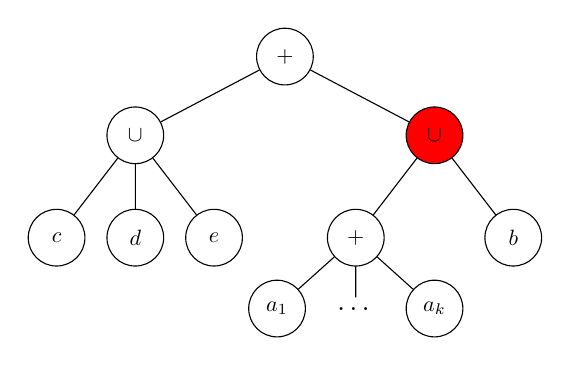
\begin{tikzpicture}[main_node/.style={circle,draw,inner sep=3pt,minimum size = 0.9cm, scale=0.8}]

	\node[main_node] (1)   at (1.1,0) {$+$};
    \node[main_node] (2)   at (-0.8, -1) {$\cup$};
	\node[main_node, fill=red] (3)   at (3,-1){$\cup$};
    \node[main_node] (4)   at (-1.8, -2.3){$c$};
    \node[main_node] (5)   at (-0.8,-2.3) {$d$};
    \node[main_node] (6)   at (0.2,-2.3) {$e$};
    \node[main_node] (7)   at (2,-2.3) {$+$};
    \node[main_node] (8)   at (4,-2.3) {$b$};
    \node[main_node] (9)   at (1,-3.2) {$a_1$};
    \node[] (10)   at (2,-3.2) {$\dots$};
     \node[main_node] (11)   at (3,-3.2) {$a_k$};
    
    \draw (4) -- (2) -- (5);
    \draw (6) -- (2) -- (1) -- (3) -- (7) -- (9);
    \draw (8) -- (3);
    \draw (10) -- (7) -- (11);

\end{tikzpicture}
\caption{Kodrevo družine kografov $G_k$ s slike~\ref{fig:counterExampleGraph}. Rdeče obarvano vozlišče ima lastnost $\mathcal{R}$.}
\label{fig:counterExampleTree}
\end{figure}

Naj bo $c$ koren kodrevesa $T_{G_k}$, ki je označen s $+$. V primeru~\ref{primerP} smo pokazali, da $T_{G_k}(c) = G_k$ zadošča lastnosti $\mathcal{P}$, saj je $\{a_1, b\}$ dominantna množica, množici $V(G) \setminus N_G[a_1] = \{b\}$ in $V(G) \setminus N_G[b] = V(K_k)$ pa sta kliki. Vendar $G_k$ ne izpolnjuje pogojev iz zgornje leme~\ref{OriginalLemma2}. Vozlišče $c$ ima v kodrevesu $T_{G_k}$ dva potomca, oba sta označena s $\cup$. Hitro se lahko prepričamo, da ima desni potomec lastnost $\mathcal{R}$, levi pa zaradi števila potomcev ne, kar pomeni, da levi potomec ni niti list niti vozlišče z oznako $\mathcal{R}$, torej pogoju v lemi~\ref{OriginalLemma2} ni zadoščeno. S tem smo našli neskončno protiprimerov za lemo~\ref{OriginalLemma2}.

Lemo smo popravili z dodatnim pogojem (lema~\ref{Lema2} $(ii)$) ter dokazali pravilnost karakterizacije, v opombi~\ref{opombaLema2} pa pokazali, da vpeljana sprememba ne spremeni linearnosti algoritma. V prvotni implementaciji za potrebe določanja lastnosti $\mathcal{P}$ za graf $T_G(c)$ namreč potrebujemo le podatek o potomcih vozlišča $c$. Zanje preverimo, če so bodisi list bodisi vozlišče z oznako $\mathcal{R}$, pri čemer smo za potrebe podatkov o lastnost $\mathcal{R}$ implementirali seznam $\mathcal{R}$, ki ga posodobimo na vsaki iteraciji v $O(|N_{T_G(ci)}(c_i)|)$ času. Popravljena lema zaradi pogoja $(ii)$ zahteva, da se preverja tudi polnost komponent potomcev vozlišča $c$. Ker za polne grafe $H$ velja $\gamma_s(H) = 1$, vrednosti $\gamma_s$ pa algoritem sproti beleži, z dodatnim pogojem ne presežemo linearnosti časovne zahtevnosti.

Izračun $\gamma_s(T_G(c))$ za spoj grafov smo tako razdelili glede na lastnost $\mathcal{P}$, v primeru, da graf lastnosti ne zadošča, pa še glede na število potomcev $c$ ter z lastnostjo $\mathcal{P^*}$ definirano funkcijo $Q(G, G_i)$. Predstavili smo način implementacije algoritma, računanja lastnosti $\mathcal{R}$ in $\mathcal{P^*}$, argumentirali linearno časovno zahtevnost algoritma PJB ter pokazali potek algoritma na primeru.
\vfill
\pagebreak

\section*{Dodatek B}
V dodatku B se nahaja implementacija algoritma PJB. Implementiranje v programskem jeziku \emph{Python} s pomočjo knjižnice \emph{SageMath}. Koda je prosto dostopna tudi na naslovu 

\subsection*{Pomožne metode}
\begin{minted}[
frame=lines,
framesep=2mm,
baselinestretch=1.2,
% bgcolor=LightGray,
fontsize=\scriptsize,
linenos
]{python}
def isLeaf(c, dict):
    ''' Input: c - node,
               dict - dictionary for U = true; + = False; None = leaf
        Output: boolean whether c is a leaf or not'''
    return dict.get(c) == None

def getChildren(c, H, Bfslist):
    '''Input: c - node,
              H - cotree,
              Bfslist - list of nodes in reverse Bfs order. 
        Output: list of children of c '''
    neighbors = H.neighbors(c)
    children = []
    for u in neighbors:
        if Bfslist.index(u) < Bfslist.index(c):
            children.append(u)
    return children

def initializeR(c, children, dict, Bfslist, R, gamma_S, gamma):
    '''Input: c - node,
              children - list of children of c,
              dict - dictionary for U = true; + = False; None = leaf,
              Bfslist - list of nodes in reverse Bfs order,
              R - old R list
        Output: new R list '''
    if dict.get(c):
        if len(children) == 2:
            if gamma_S[Bfslist.index(children[0])] == 1 and gamma[Bfslist.index(children[1])] == 1:
                R[Bfslist.index(c)] = 1
            if gamma_S[Bfslist.index(children[1])] == 1 and gamma[Bfslist.index(children[0])] == 1:
                R[Bfslist.index(c)] = 1
    return R

def initializeA (c, children, dict, Bfslist, A, R):
    '''Input: c - node,
              children - list of children of c,
              dict - dictionary for U = true; + = False; None = leaf,
              Bfslist - list of nodes in reverse Bfs order,
              A - old A* list
        Output: new A* list '''
    if isLeaf(c, dict):
        A[Bfslist.index(c)] = 1
    if dict.get(c) == False:
        allChildrenLeaves = false
        nonLeafChildren = false
        hasR = false
        for u in children:
            if isLeaf(c, dict):
                nonLeafChildren = True
            else:
                allChildrenLeaves = True
            if R[Bfslist.index(u)] == 1:
                hasR = True
        if allChildrenLeaves:
            A[Bfslist.index(c)] = 1
        if nonLeafChildren and hasR:
            A[Bfslist.index(c)] = 1
    return A
    
def initializeRstar (c, Bfslist, A, Rstar, children):
    '''Input: c - node,
              children - list of children of c,
              dict - dictionary for U = true; + = False; None = leaf,
              Bfslist - list of nodes in reverse Bfs order,
              A - A* list,
              Rstar - old R* list
        Output: new R* list '''
    for u in children:
        if A[Bfslist.index(u)] == 1:
            Rstar[Bfslist.index(c)] = 1
    return Rstar

def initializeGamma(c, children, dict, Bfslist, gamma):
    '''Input: c - node,
              children - list of children of c,
              dict - dictionary for U = true; + = False; None = leaf,
              Bfslist - list of nodes in reverse Bfs order,
              gamma - old $\gamma$ list
        Output: new gamma list '''
    if isLeaf(c, dict):
        gamma[Bfslist.index(c)] = 1
    if dict.get(c):
        for u in children:
            gamma[Bfslist.index(c)] += gamma[Bfslist.index(u)]
    if not dict.get(c):
        if atLeastOneChildIsALeaf:
            gamma[Bfslist.index(c)] = 1
        else:
            gamma[Bfslist.index(c)] = 2
    return gamma
        

def allChildrenAreLeaves(children, dict):
    '''Input: children - list of nodes,
              dict - dictionary for U = true; + = False; None = leaf
        Output: boolean '''
    allLeaves = true
    for u in children:
        if not isLeaf(u, dict):
            allLeaves = false
            break;
    return allLeaves

def atLeastOneChildIsALeaf(children, dict):
    '''Input: children - list of nodes,
              dict - dictionary for U = true; + = False; None = leaf
       Output: boolean '''
    for u in children:
        if isLeaf(u, dict):
            return True
    return False

def doesTGcsatisfyPropertyP(c, children, dict, gamma_S, R, Bfslist, H):
    '''Input: c - node, 
              children - list of nodes,
              dict - dictionary for U = true; + = False; None = leaf,
              gamma_S - list of $\gamma_S$,
              R - list R,
              Bfslist - list of nodes in reverse Bfs order,
              H - cotree
       Output: boolean whether $T_G(c)$ satisfies property $\mathcal{P}$ or not'''
    counterL = 0
    counterR = 0
    counterS = 0
    for u in children:
        if isLeaf(u, dict):
            counterL += 1
        if R[Bfslist.index(u)] == 1:
            counterR += 1
        if counterL + counterR == 2:
            return True
        
        if dict.get(u):
            subchildren = getChildren(u, H, Bfslist)
            if len(subchildren) == 2:
                if gamma_S[Bfslist.index(subchildren[0])] == 1 and
                gamma_S[Bfslist.index(subchildren[1])] == 1:
                    counterS += 1
        if counterR == 1 and counterS == 1:
            return True
    return False

def calculateQ(c, children, Rstar, gamma, Bfslist):
    '''Input: c - node, 
              children - list of nodes,
              gamma - list of $\gamma$,
              Rstar - list $\mathcal{R}$,
              Bfslist - list of nodes in reverse Bfs order
       Output: computes $Q(T_G(c), ...)$'''
    Q = 0
    for u in children:
        Q += gamma[Bfslist.index(u)]
    if Rstar[Bfslist.index(c)] == 1:
        return Q
    else:
        return Q + 1
\end{minted}

%%%%%%%%%%%%%%%%%%%%%%%%%%%%%
%%%%%%%%%%%%%%%%%%%%%%%%%%%%%
%%%%%%%%%%%%%%%%%%%%%%%%%%%%%

\subsection*{Algoritem PJB}

\begin{minted}[
frame=lines,
framesep=2mm,
baselinestretch=1.2,
% bgcolor=LightGray,
fontsize=\scriptsize,
linenos
]{python}

def isciGammaS(H, dict, root):
    '''Input: H - cotree, 
              dict - dictionary for U = true; + = False; None = leaf,
              root - root of cotree H
       Output: $\gamma_S(H)$'''
    Bfslist = H.lex_BFS(initial_vertex=root, reverse=True)
    gamma_S = len(Bfslist) * [0]
    gamma = len(Bfslist) * [0]
    R = len(Bfslist) * [0]
    A = len(Bfslist) * [0]
    Rstar = len(Bfslist) * [0]
    for c in Bfslist:
        children = getChildren(c, H, Bfslist)
        R = initializeR(c, children, dict, Bfslist, R, gamma_S, gamma)
        A = initializeA (c, children, dict, Bfslist, A, R)
        Rstar = initializeRstar (c, Bfslist, A, Rstar, children)
        initializeGamma(c, dict, Bfslist, gamma, children)
        
        if isLeaf(c, dict):                                             # c is leaf
            gamma_S[Bfslist.index(c)] = 1
        elif dict.get(c):                                               # c has label U
            for u in children:
                gamma_S[Bfslist.index(c)] += gamma_S[Bfslist.index(u)]
        elif not dict.get(c):                                           # c has label +
            if allChildrenAreLeaves(children, dict):
                gamma_S[Bfslist.index(c)] = 1
            elif doesTGcsatisfyPropertyP(c, children, dict, gamma_S, R, Bfslist, H):
                                                                        #T_G(c) has property P
                gamma_S[Bfslist.index(c)] = 2
            elif len(children) >= 3:
                gamma_S[Bfslist.index(c)] = 3
            elif isLeaf(children[0], dict) and not isLeaf(children[1], dict):
                gamma_S[Bfslist.index(c)] = calculateQ(
                    children[1], getChildren(children[1], H, Bfslist), Rstar, gamma, Bfslist)
            elif isLeaf(children[1], dict) and not isLeaf(children[0], dict):
                gamma_S[Bfslist.index(c)] = calculateQ(
                    children[0], getChildren(children[0], H, Bfslist), Rstar, gamma, Bfslist)
            else:
                u1 = children[0]
                u2 = children[1]
                if (calculateQ(u1, getChildren(u1, H, Bfslist)) == 3 or
                    calculateQ(u2, getChildren(u2, H, Bfslist)) == 3 or
                    gamma_S[Bfslist.index(u1)] == 3 or
                    gamma_S[Bfslist.index(u2)] == 3):
                    gamma_S[Bfslist.index(c)] = 3
                else:
                    gamma_S[Bfslist.index(c)] = 4
                                                                                 
    return gamma_S

\end{minted}
\pagebreak


% Literatura:
\begin{thebibliography}{99}

\bibitem{allem2020integral}
    L.E.~Allem, F.~Tura,
    Integral cographs,
    Discrete Applied Mathematics 283 (2020) 153--167. 
    
\bibitem{araki2018secure}
    T.~Araki, H.~Miyazaki,
    Secure domination in proper interval graphs,
    Discrete Applied Mathematics 247 (2018) 70--76.
    
\bibitem{araki2019secure}
    T. Araki, R. Yamanaka,
    Secure domination in cographs,
    Discrete Applied Mathematics 262 (2019) 179--184.
    
\bibitem{berge1961coloring}
    C.~Berge,
    F\"{a}rbung von Graphen, deren s\"{a}mtliche bzw. deren ungerade Kreise Starr sind,
    Wiss. Z. Martin Luther Univ. Halle Wittenberg Math. Natur. Reihe 10 (1961), 114.
    
\bibitem{brevsar2015cographs}
    B.~Brešar, T.~Gologranc, M.~Manoj, B.~Sukumaran,
    Cographs which are cover-incomparability graphs of posets,
    Order 32 (2015) 179--187.

\bibitem{burdett2020improved}
    R.~Burdett, M.~Haythorpe,
    An improved binary programming formulation for the secure domination problem,
    Annals of Operations Research (2020) https://doi.org/10.1007/s10479-020-03810-6.

\bibitem{burger2013binary}
    A.P.~Burger, A.P.~de Villiers, J.H.~van Vuuren,
    A binary programming approach towards achieving effective graph protection,
    Proc. 2013 ORSSA Annual Conference, ORSSA (2013) 19--30.

\bibitem{burger2014linear}
    A.P.~Burger, A.P.~de Villiers, J.H.~van Vuuren,
    A linear algorithm for secure domination in trees,
    Discrete Applied Mathematics 171 (2014) 12--27.

\bibitem{castillano2014secure}
    E.C.~Castillano, R.L.~Ugibanda, S.R.~Canoy Jr,
    Secure domination in the join of graphs,
    Applied Mathematical Sciences 8 (2014) 5203--5211.
   
\bibitem{christen1979some}
    C.A.~Christen, S.M.~Selkow,
    Some perfect coloring properties of graphs,
    Journal of Combinatorial Theory 27 (1979) 49--59.
    
\bibitem{chudnovsky2006strong}
    M.~Chudnovsky, N.~Robertson, P.~Seymour, R.~Thomas,
    The strong perfect graph theorem,
    Annals of Mathematics (2006) 51--229.
    
\bibitem{cockayne2005protection}
    E.J.~Cockayne, P.J.P.~Grobler, W.R.~Grundlingh, J.~Munganga, J.H.~van Vuuren,
    Protection of a graph,
    Utilitas Mathematica 67 (2005) 19--32.
    
\bibitem{cockayne1977towards}
    E.J.~Cockayne, S.T.~Hedetniemi,
    Towards a theory of domination in graphs,
    Networks 7 (1977) 247--261.
    
\bibitem{corneil1981complement}
    D.G.~Corneil, H.~Lerchs, L.~Stewart Burlingham,
    Complement reducible graphs,
    Discrete Applied Mathematics 3 (1981) 163--174.
    
\bibitem{corneil1985linear}
    D.G.~Conrenil, Y.~Perl, L.K.~Stewart,
    A linear recognition algorithm for cographs,
    SIAM Journal on Computing 14 (1985) 926--934.
   
\bibitem{corneil1984cographs}
    D.G.~Corneil, Y.~Perl,
    Cographs: recognition, applications and algorithms,
    Congressus Numerantium 43 (1984) 249--258.
    
\bibitem{corneil1984clustering}
    D.G.~Corneil, Y.~Perl,
    Clustering and domination in perfect graphs,
    Discrete Applied Mathematics 9 (1984) 27--39.
    
\bibitem{epple2020k}
    D.A.~Epple, J.~Huang,
    $(k, l)$-colourings and Ferrers diagram representations of cographs,
    European Journal of Combinatorics 91 (2020) Paper 103208.
    
\bibitem{geiss2020reciprocal}
    M.~Gei{\ss}, P.F.~Stadler, M.~Hellmuth,
    Reciprocal best match graphs,
    Journal of Mathematical Biology 80 (2020) 865--953.
    
\bibitem{ghorbani2019cographs}
    E.~Ghorbani,
    Cographs: eigenvalues and Dilworth number,
    Discrete Mathematics 342 (2019) 2797--2803.

\bibitem{hellmuth2013orthology}
    M.~Hellmuth, M.~Hernandez-Rosales, K.T.~Huber, V.~Moulton, P.F.~Stadler, N.~Weiseke,
    Orthology relations, symbolic ultrametrics, and cographs,
    Journal of mathematical biology 66 (2013) 399--420.

\bibitem{jha2019secure}
  A.~Jha, D.~Pradhan, S.~Banerjee, 
  The secure domination problem in cographs,
  Information Processing Letters 145 (2019) 30--38.
  
\bibitem{karp1972reducibility}
    R.M.~Karp,
    Reducibility among combinatorial problems,
    Complexity of computer computations (1972) 85--103.
    
\bibitem{kisek2020onJha}
    A.~Kišek, S.~Klavžar,
    On the Jha/Pradhan/Banerjee algorithm for the secure domination number of cographs,
    arXiv preprint arXiv:2011.00522 (2020).
    
\bibitem{li2017secure}
    Z.~Li, Z.~Shao, J.~Xu,
    On secure domination in trees,
    Quaestiones Mathematicae 40 (2017) 1--12.
    
\bibitem{lovasz1972characterisation}
    L.~Lovász,
    A characterization of perfect graphs,
    Journal of Combinatorial Theory, Series B 13 (1972) 95--98.
    
\bibitem{maffray2003coloration}
    F.~Maffray,
    On the coloration of perfect graphs,
    Recent Advances in Algorithms and Combinatorics (2003) 65--84.
 
\bibitem{merouane2015secure}
    H.B.~Merouane, M.~Chellali,
    On secure domination in graphs,
    Information Processing Letters 115 (2015) 786--790.
    
\bibitem{ore1962theory}
    O.~Ore,
    Theory of Graphs,
    American Mathematical Society Colloquium Publications 38 (1962).

\bibitem{pavlic2010rimsko}
    P.~Pavlič, J.~Žerovnik,
    Rimsko dominantno število,
    Obzornik za matematiko in fiziko 60 (2013) 121--128.
    
\bibitem{pradhan2018computing}
    D.~Pradhan, A.~Jha,
    On computing a minimum secure dominating set in block graphs,
    Journal of Combinatorial Optimization 35 (2018) 613--631.
    
\bibitem{seinsche1974property}
    D.~Seinsche,
    On a property of the class of n-colorable graphs,
    Journal of Combinatorial Theory, Series B 16 (1974) 191--193.
    
\bibitem{stewart1978cographs}
    L.~Stewart,
    Cographs: a class of tree representable graphs,
    PhD thesis,
    University of Toronto, Department of Computer Science (1978).
    
\bibitem{stewart1999defend}
    I.~Stewart,
    Defend the Roman empire!,
    Scientific American 281 (1999) 136--138.
    
\bibitem{tsur2020faster}
    D.~Tsur,
    Faster algorithms for cograph edge modification problems,
    Information Processing Letters 158 (2020) Paper 105946. 

\bibitem{wang2018complexity}
    H.~Wang, Y.~Zhao, Y.~Deng,
    The complexity of secure domination problem in graphs,
    Discussiones Mathematicae Graph Theory 38 (2018) 385--396.
    
\bibitem{yu1993n}
    M.~Yu, C.~Yang,
    An $O(n)$ time algorithm for maximum matching on cographs,
    Information processing letters 47 (1993) 89--93.
    
\end{thebibliography}



% Za stvarno kazalo
\cleardoublepage                           % na desni strani
\phantomsection                            % da prav delujejo hiperlinki
\addcontentsline{toc}{section}{\indexname} % dodajmo v kazalo
\printindex

\end{document}
